%%  JLG input 2/18/2017 
%% TGARS Draft - JLG input 8/11/2016
%%bare_jrnl.tex
%% V1.4a
%% 2014/09/17
%% by Michael Shell
%% see http://www.michaelshell.org/
%% for current contact information.
%%
%% This is a skeleton file demonstrating the use of IEEEtran.cls
%% (requires IEEEtran.cls version 1.8a or later) with an IEEE
%% journal paper.
%%
%% Support sites:
%% http://www.michaelshell.org/tex/ieeetran/
%% http://www.ctan.org/tex-archive/macros/latex/contrib/IEEEtran/
%% and
%% http://www.ieee.org/

%%************************************************************************
%% Legal Notice:
%% This code is offered as-is without any warranty either expressed or
%% implied; without even the implied warranty of MERCHANTABILITY or
%% FITNESS FOR A PARTICULAR PURPOSE! 
%% User assumes all risk.
%% In no event shall IEEE or any contributor to this code be liable for
%% any damages or losses, including, but not limited to, incidental,
%% consequential, or any other damages, resulting from the use or misuse
%% of any information contained here.
%%
%% All comments are the opinions of their respective authors and are not
%% necessarily endorsed by the IEEE.
%%
%% This work is distributed under the LaTeX Project Public License (LPPL)
%% ( http://www.latex-project.org/ ) version 1.3, and may be freely used,
%% distributed and modified. A copy of the LPPL, version 1.3, is included
%% in the base LaTeX documentation of all distributions of LaTeX released
%% 2003/12/01 or later.
%% Retain all contribution notices and credits.
%% ** Modified files should be clearly indicated as such, including  **
%% ** renaming them and changing author support contact information. **
%%
%% File list of work: IEEEtran.cls, IEEEtran_HOWTO.pdf, bare_adv.tex,
%%                    bare_conf.tex, bare_jrnl.tex, bare_conf_compsoc.tex,
%%                    bare_jrnl_compsoc.tex, bare_jrnl_transmag.tex
%%*************************************************************************


% *** Authors should verify (and, if needed, correct) their LaTeX system  ***
% *** with the testflow diagnostic prior to trusting their LaTeX platform ***
% *** with production work. IEEE's font choices and paper sizes can       ***
% *** trigger bugs that do not appear when using other class files.       ***                          ***
% The testflow support page is at:
% http://www.michaelshell.org/tex/testflow/



\documentclass[draftcls,onecolumn]{IEEEtran}  % JLG -recommend one-column for drafts

\bibliographystyle{IEEEtran}

%
% If IEEEtran.cls has not been installed into the LaTeX system files,
% manually specify the path to it like:
% \documentclass[journal]{../sty/IEEEtran}





% Some very useful LaTeX packages include:
% (uncomment the ones you want to load)


% *** MISC UTILITY PACKAGES ***
%
%\usepackage{ifpdf}
% Heiko Oberdiek's ifpdf.sty is very useful if you need conditional
% compilation based on whether the output is pdf or dvi.
% usage:
% \ifpdf
%   % pdf code
% \else
%   % dvi code
% \fi
% The latest version of ifpdf.sty can be obtained from:
% http://www.ctan.org/tex-archive/macros/latex/contrib/oberdiek/
% Also, note that IEEEtran.cls V1.7 and later provides a builtin
% \ifCLASSINFOpdf conditional that works the same way.
% When switching from latex to pdflatex and vice-versa, the compiler may
% have to be run twice to clear warning/error messages.






% *** CITATION PACKAGES ***
%
%\usepackage{cite}
% cite.sty was written by Donald Arseneau
% V1.6 and later of IEEEtran pre-defines the format of the cite.sty package
% \cite{} output to follow that of IEEE. Loading the cite package will
% result in citation numbers being automatically sorted and properly
% "compressed/ranged". e.g., [1], [9], [2], [7], [5], [6] without using
% cite.sty will become [1], [2], [5]--[7], [9] using cite.sty. cite.sty's
% \cite will automatically add leading space, if needed. Use cite.sty's
% noadjust option (cite.sty V3.8 and later) if you want to turn this off
% such as if a citation ever needs to be enclosed in parenthesis.
% cite.sty is already installed on most LaTeX systems. Be sure and use
% version 5.0 (2009-03-20) and later if using hyperref.sty.
% The latest version can be obtained at:
% http://www.ctan.org/tex-archive/macros/latex/contrib/cite/
% The documentation is contained in the cite.sty file itself.






% *** GRAPHICS RELATED PACKAGES ***
%
\ifCLASSINFOpdf
   \usepackage[pdftex]{graphicx}
  % declare the path(s) where your graphic files are
   \graphicspath{{../pdf/}{../jpeg/}}
  % and their extensions so you won't have to specify these with
  % every instance of \includegraphics
   \DeclareGraphicsExtensions{.pdf,.jpeg,.png}
\else
  % or other class option (dvipsone, dvipdf, if not using dvips). graphicx
  % will default to the driver specified in the system graphics.cfg if no
  % driver is specified.
  % \usepackage[dvips]{graphicx}
  % declare the path(s) where your graphic files are
  % \graphicspath{{../eps/}}
  % and their extensions so you won't have to specify these with
  % every instance of \includegraphics
  % \DeclareGraphicsExtensions{.eps}
\fi
% graphicx was written by David Carlisle and Sebastian Rahtz. It is
% required if you want graphics, photos, etc. graphicx.sty is already
% installed on most LaTeX systems. The latest version and documentation
% can be obtained at: 
% http://www.ctan.org/tex-archive/macros/latex/required/graphics/
% Another good source of documentation is "Using Imported Graphics in
% LaTeX2e" by Keith Reckdahl which can be found at:
% http://www.ctan.org/tex-archive/info/epslatex/
%
% latex, and pdflatex in dvi mode, support graphics in encapsulated
% postscript (.eps) format. pdflatex in pdf mode supports graphics
% in .pdf, .jpeg, .png and .mps (metapost) formats. Users should ensure
% that all non-photo figures use a vector format (.eps, .pdf, .mps) and
% not a bitmapped formats (.jpeg, .png). IEEE frowns on bitmapped formats
% which can result in "jaggedy"/blurry rendering of lines and letters as
% well as large increases in file sizes.
%
% You can find documentation about the pdfTeX application at:
% http://www.tug.org/applications/pdftex


\usepackage{diagbox}


% *** MATH PACKAGES ***
%
\usepackage[cmex10]{amsmath}
% A popular package from the American Mathematical Society that provides
% many useful and powerful commands for dealing with mathematics. If using
% it, be sure to load this package with the cmex10 option to ensure that
% only type 1 fonts will utilized at all point sizes. Without this option,
% it is possible that some math symbols, particularly those within
% footnotes, will be rendered in bitmap form which will result in a
% document that can not be IEEE Xplore compliant!
%
% Also, note that the amsmath package sets \interdisplaylinepenalty to 10000
% thus preventing page breaks from occurring within multiline equations. Use:
%\interdisplaylinepenalty=2500
% after loading amsmath to restore such page breaks as IEEEtran.cls normally
% does. amsmath.sty is already installed on most LaTeX systems. The latest
% version and documentation can be obtained at:
% http://www.ctan.org/tex-archive/macros/latex/required/amslatex/math/





% *** SPECIALIZED LIST PACKAGES ***
%
\usepackage{algorithmic}
% algorithmic.sty was written by Peter Williams and Rogerio Brito.
% This package provides an algorithmic environment fo describing algorithms.
% You can use the algorithmic environment in-text or within a figure
% environment to provide for a floating algorithm. Do NOT use the algorithm
% floating environment provided by algorithm.sty (by the same authors) or
% algorithm2e.sty (by Christophe Fiorio) as IEEE does not use dedicated
% algorithm float types and packages that provide these will not provide
% correct IEEE style captions. The latest version and documentation of
% algorithmic.sty can be obtained at:
% http://www.ctan.org/tex-archive/macros/latex/contrib/algorithms/
% There is also a support site at:
% http://algorithms.berlios.de/index.html
% Also of interest may be the (relatively newer and more customizable)
% algorithmicx.sty package by Szasz Janos:
% http://www.ctan.org/tex-archive/macros/latex/contrib/algorithmicx/




% *** ALIGNMENT PACKAGES ***
%
\usepackage{array}
% Frank Mittelbach's and David Carlisle's array.sty patches and improves
% the standard LaTeX2e array and tabular environments to provide better
% appearance and additional user controls. As the default LaTeX2e table
% generation code is lacking to the point of almost being broken with
% respect to the quality of the end results, all users are strongly
% advised to use an enhanced (at the very least that provided by array.sty)
% set of table tools. array.sty is already installed on most systems. The
% latest version and documentation can be obtained at:
% http://www.ctan.org/tex-archive/macros/latex/required/tools/


% IEEEtran contains the IEEEeqnarray family of commands that can be used to
% generate multiline equations as well as matrices, tables, etc., of high
% quality.

% *** SUBFIGURE PACKAGES ***
%\ifCLASSOPTIONcompsoc
%  \usepackage[caption=false,font=normalsize,labelfont=sf,textfont=sf]{subfig}
%\else
%  \usepackage[caption=false,font=footnotesize]{subfig}
%\fi
% subfig.sty, written by Steven Douglas Cochran, is the modern replacement
% for subfigure.sty, the latter of which is no longer maintained and is
% incompatible with some LaTeX packages including fixltx2e. However,
% subfig.sty requires and automatically loads Axel Sommerfeldt's caption.sty
% which will override IEEEtran.cls' handling of captions and this will result
% in non-IEEE style figure/table captions. To prevent this problem, be sure
% and invoke subfig.sty's "caption=false" package option (available since
% subfig.sty version 1.3, 2005/06/28) as this is will preserve IEEEtran.cls
% handling of captions.
% Note that the Computer Society format requires a larger sans serif font
% than the serif footnote size font used in traditional IEEE formatting
% and thus the need to invoke different subfig.sty package options depending
% on whether compsoc mode has been enabled.
%
% The latest version and documentation of subfig.sty can be obtained at:
% http://www.ctan.org/tex-archive/macros/latex/contrib/subfig/




% *** FLOAT PACKAGES ***
%
%\usepackage{fixltx2e}
% fixltx2e, the successor to the earlier fix2col.sty, was written by
% Frank Mittelbach and David Carlisle. This package corrects a few problems
% in the LaTeX2e kernel, the most notable of which is that in current
% LaTeX2e releases, the ordering of single and double column floats is not
% guaranteed to be preserved. Thus, an unpatched LaTeX2e can allow a
% single column figure to be placed prior to an earlier double column
% figure. The latest version and documentation can be found at:
% http://www.ctan.org/tex-archive/macros/latex/base/


%\usepackage{stfloats}
% stfloats.sty was written by Sigitas Tolusis. This package gives LaTeX2e
% the ability to do double column floats at the bottom of the page as well
% as the top. (e.g., "\begin{figure*}[!b]" is not normally possible in
% LaTeX2e). It also provides a command:
%\fnbelowfloat
% to enable the placement of footnotes below bottom floats (the standard
% LaTeX2e kernel puts them above bottom floats). This is an invasive package
% which rewrites many portions of the LaTeX2e float routines. It may not work
% with other packages that modify the LaTeX2e float routines. The latest
% version and documentation can be obtained at:
% http://www.ctan.org/tex-archive/macros/latex/contrib/sttools/
% Do not use the stfloats baselinefloat ability as IEEE does not allow
% \baselineskip to stretch. Authors submitting work to the IEEE should note
% that IEEE rarely uses double column equations and that authors should try
% to avoid such use. Do not be tempted to use the cuted.sty or midfloat.sty
% packages (also by Sigitas Tolusis) as IEEE does not format its papers in
% such ways.
% Do not attempt to use stfloats with fixltx2e as they are incompatible.
% Instead, use Morten Hogholm'a dblfloatfix which combines the features
% of both fixltx2e and stfloats:
%
% \usepackage{dblfloatfix}
% The latest version can be found at:
% http://www.ctan.org/tex-archive/macros/latex/contrib/dblfloatfix/




%\ifCLASSOPTIONcaptionsoff
%  \usepackage[nomarkers]{endfloat}
% \let\MYoriglatexcaption\caption
% \renewcommand{\caption}[2][\relax]{\MYoriglatexcaption[#2]{#2}}
%\fi
% endfloat.sty was written by James Darrell McCauley, Jeff Goldberg and 
% Axel Sommerfeldt. This package may be useful when used in conjunction with 
% IEEEtran.cls'  captionsoff option. Some IEEE journals/societies require that
% submissions have lists of figures/tables at the end of the paper and that
% figures/tables without any captions are placed on a page by themselves at
% the end of the document. If needed, the draftcls IEEEtran class option or
% \CLASSINPUTbaselinestretch interface can be used to increase the line
% spacing as well. Be sure and use the nomarkers option of endfloat to
% prevent endfloat from "marking" where the figures would have been placed
% in the text. The two hack lines of code above are a slight modification of
% that suggested by in the endfloat docs (section 8.4.1) to ensure that
% the full captions always appear in the list of figures/tables - even if
% the user used the short optional argument of \caption[]{}.
% IEEE papers do not typically make use of \caption[]'s optional argument,
% so this should not be an issue. A similar trick can be used to disable
% captions of packages such as subfig.sty that lack options to turn off
% the subcaptions:
% For subfig.sty:
% \let\MYorigsubfloat\subfloat
% \renewcommand{\subfloat}[2][\relax]{\MYorigsubfloat[]{#2}}
% However, the above trick will not work if both optional arguments of
% the \subfloat command are used. Furthermore, there needs to be a
% description of each subfigure *somewhere* and endfloat does not add
% subfigure captions to its list of figures. Thus, the best approach is to
% avoid the use of subfigure captions (many IEEE journals avoid them anyway)
% and instead reference/explain all the subfigures within the main caption.
% The latest version of endfloat.sty and its documentation can obtained at:
% http://www.ctan.org/tex-archive/macros/latex/contrib/endfloat/
%
% The IEEEtran \ifCLASSOPTIONcaptionsoff conditional can also be used
% later in the document, say, to conditionally put the References on a 
% page by themselves.




% *** PDF, URL AND HYPERLINK PACKAGES ***
%
%\usepackage{url}
% url.sty was written by Donald Arseneau. It provides better support for
% handling and breaking URLs. url.sty is already installed on most LaTeX
% systems. The latest version and documentation can be obtained at:
% http://www.ctan.org/tex-archive/macros/latex/contrib/url/
% Basically, \url{my_url_here}.




% *** Do not adjust lengths that control margins, column widths, etc. ***
% *** Do not use packages that alter fonts (such as pslatex).         ***
% There should be no need to do such things with IEEEtran.cls V1.6 and later.
% (Unless specifically asked to do so by the journal or conference you plan
% to submit to, of course. )

% correct bad hyphenation here
\hyphenation{op-tical net-works semi-conduc-tor}


\begin{document}
%
% paper title
% Titles are generally capitalized except for words such as a, an, and, as,
% at, but, by, for, in, nor, of, on, or, the, to and up, which are usually
% not capitalized unless they are the first or last word of the title.
% Linebreaks \\ can be used within to get better formatting as desired.
% Do not put math or special symbols in the title.
\title{An Airborne Demonstrator for Remote Sensing of Root Zone Soil Moisture (RZSM) using P-band Signals of Opportunity (SoOp)}
%
%
% author names and IEEE memberships
% note positions of commas and nonbreaking spaces ( ~ ) LaTeX will not break
% a structure at a ~ so this keeps an author's name from being broken across
% two lines.
% use \thanks{} to gain access to the first footnote area
% a separate \thanks must be used for each paragraph as LaTeX2e's \thanks
% was not built to handle multiple paragraphs
%

\author{James~L. Garrison,~\IEEEmembership{Senior Member,~IEEE}
        Yao-Cheng~Lin,~\IEEEmembership{Member,~IEEE},
        Jeffrey Piepmeier,~\IEEEmembership{Senior Member,~IEEE},
        Joesph Knuble,~\IEEEmembership{Senior Member,~IEEE},
        Manuel A. Vega,~\IEEEmembership{Member,~IEEE},
        Georges~Stienne,~\IEEEmembership{Member,~IEEE}
        and~Cornelis~Frederik~du~Toit,~\IEEEmembership{Senior Member,~IEEE}% <-this % stops a space
\thanks{Yao-Cheng Lin is with Aeronautics and Astronautics, Purdue University, Indiana,
IN, 47907}}

% note the % following the last \IEEEmembership and also \thanks - 
% these prevent an unwanted space from occurring between the last author name
% and the end of the author line. i.e., if you had this:
% 
% \author{....lastname \thanks{...} \thanks{...} }
%                     ^------------^------------^----Do not want these spaces!
%
% a space would be appended to the last name and could cause every name on that
% line to be shifted left slightly. This is one of those "LaTeX things". For
% instance, "\textbf{A} \textbf{B}" will typeset as "A B" not "AB". To get
% "AB" then you have to do: "\textbf{A}\textbf{B}"
% \thanks is no different in this regard, so shield the last } of each \thanks
% that ends a line with a % and do not let a space in before the next \thanks.
% Spaces after \IEEEmembership other than the last one are OK (and needed) as
% you are supposed to have spaces between the names. For what it is worth,
% this is a minor point as most people would not even notice if the said evil
% space somehow managed to creep in.



% The paper headers
\markboth{Journal of \LaTeX\ Class Files,~Vol.~13, No.~9, September~2014}%
{Shell \MakeLowercase{\textit{et al.}}: Bare Demo of IEEEtran.cls for Journals}
% The only time the second header will appear is for the odd numbered pages
% after the title page when using the twoside option.
% 
% *** Note that you probably will NOT want to include the author's ***
% *** name in the headers of peer review papers.                   ***
% You can use \ifCLASSOPTIONpeerreview for conditional compilation here if
% you desire.




% If you want to put a publisher's ID mark on the page you can do it like
% this:
%\IEEEpubid{0000--0000/00\$00.00~\copyright~2014 IEEE}
% Remember, if you use this you must call \IEEEpubidadjcol in the second
% column for its text to clear the IEEEpubid mark.



% use for special paper notices
%\IEEEspecialpapernotice{(Invited Paper)}




% make the title area
\maketitle

% As a general rule, do not put math, special symbols or citations
% in the abstract or keywords.
\begin{abstract}
Signals of Opportunity Airborne Demonstrator (SoOp-AD), a NASA Instrument Incubator Program (IIP-13) selection, 
is designed to demonstrate remote sensing of Root Zone Soil Moisture (RZSM) using reflected communication satellite ``signals of opportunity'' (SoOp). 
Under most circumstances, the sensing depth of P-band (250 to 500 MHz) radiation is decimeters.
This enables direct measurement of  most of the water content in the very important root zone (top 1~m). 
Reutilization of existing powerful transmissions allows measurements to be made in these frequencies which would be infeasible with conventional radars or radiometers due to antenna size, limited spectrum allocation, or radio frequency interference (RFI). 
Three basic observations will be produced from this instrument: autocorrelation of the direct line-of-sight signal from the transmitter, autocorrelation of the reflected signal, and the complex cross-correlation between the direct and reflected signals, each at multiple delays and two polarizations. 
An observable is computed from the cross-correlation and the direct signal auto-correlation.
This observable is shown to be a complex function of the surface reflectivity and the path delay.
It can easily be inverted to provide estimates of these two variables. 
Emissivity (and thus reflectivity) is related to the soil moisture through well established relationships. 
P-band reflections are assumed to be nearly specular for most topographies. 
Surface resolution is thus set by the first Fresnel zone ($\approx$ 100's of m from aircraft, 1-3~km from satellite).
Furthermore, satellite transmissions in this band generally have very low bandwidth (5-25 kHz channels) and an 
airworthy antenna designed for this wavelength would have a very wide beamwidth. 
These considerations preclude relying upon delay, in contrast to Global Navigation Satellite System Reflectometry  (GNSS-R), or a narrow antenna beam to provide strong isolation between direct and reflected ray paths. Consequently, both the sky-view and Earth-view antennas would receive a combination of direct and reflected signals. The observable and inversion algorithms for the retrieval of reflectivity incorporate an understanding of this interference. 
A sensitivity study was conducted, to evaluate the dependence of retrieval accuracy on the uncertainty in antenna gain pattern, aircraft attitude, and receiver calibration.
Knowledge of the antenna gain, in the direct and reflected ray directions was determined to have the largest impact on the system error budget. 
Maximum coherent integration time was found to be limited by aircraft height variation. 
A sample-level signal simulator was developed for validating these error analyses and evaluating system performance. 
These studies were used to define system requirements to meet a working science requirement of 0.04~m$^3$/m$^3$ root mean square error (RMSE) equal to that of the Soil Moisture Active Passive (SMAP) project. 
%Fundamental considerations for the feasibility of a satellite are presented, based upon these studies. 

\end{abstract}

% Note that keywords are not normally used for peerreview papers.
\begin{IEEEkeywords}
Remote sensing, Signal of opportunity, soil moisture, P-band.
\end{IEEEkeywords}


% For peer review papers, you can put extra information on the cover
% page as needed:
% \ifCLASSOPTIONpeerreview
% \begin{center} \bfseries EDICS Category: 3-BBND \end{center}
% \fi
%
% For peerreview papers, this IEEEtran command inserts a page break and
% creates the second title. It will be ignored for other modes.
\IEEEpeerreviewmaketitle

\section{Introduction}
% The very first letter is a 2 line initial drop letter followed
% by the rest of the first word in caps.
% 
% form to use if the first word consists of a single letter:
% \IEEEPARstart{A}{demo} file is ....
% 
% form to use if you need the single drop letter followed by
% normal text (unknown if ever used by IEEE):
% \IEEEPARstart{A}{}demo file is ....
% 
% Some journals put the first two words in caps:
% \IEEEPARstart{T}{his demo} file is ....
% 
% Here we have the typical use of a "T" for an initial drop letter
% and "HIS" in caps to complete the first word.
\IEEEPARstart{S}{oil} moisture, identified by the World Meteorological Organization as an Essential Climate Variable (ECV) \cite{WMO2011}, 
plays a critical role in the Earth's hydrosphere.
Root zone soil moisture (RZSM), in particular, controls hydrologic fluxes linking surface and subsurface processes and the interplay between  water and carbon cycles.  Improved estimates of this variable would greatly improve our understanding and prediction of multiple Earth system processes. 

Weather forecast skill, for example, is very sensitive to uncertainty in soil moisture. 
In the Global Land Atmosphere Coupling Experiment (GLACE)  \cite{Glace1995} multiple simulations were performed to identify regions where global soil moisture initialization would enhance precipitation forecast skill, 
concluding that routine monitoring of soil moisture will offer the largest improvement in boreal summer seasonal forecasting.  

Simultaneous knowledge of deep (order 0.1 to 2 m) and shallow (order 0.01 to 0.1 m) soil moisture profiles can also provide a major breakthrough for estimation of two key unobserved hydrologic fluxes, evapotranspiration (ET) and aquifer recharge \cite{Entekhabi2006}.  
These processes are not well observed, but play a key role in water storage and transfer, connecting slow and fast components of water cycle. 
Spatial scales are set by heterogeneity of soil and vegetation (0.1 to 10~km) whereas temporal scales are related to precipitation and dry-down (1-3~days). 


Integration of  spatially and temporally resolved RZSM into ecosystem dynamic models is also expected to reduce the uncertainty in estimates of net ecosystem exchange (NEE) and Carbon balance \cite{Briggs2008}, \cite{Krishnan2006}. 
%Current estimates of NEE can show differences of 100\% between 11 models, an uncertainty so large that  it is not even clear if North America is net sink or source of Carbon.  
This problem motivated  AirMOSS \cite{Tabatabaeenejad2015}, a P-band SAR experiment conducted over nine (9) biomes across North America. 


RZSM was also identified  as a priority in a recent review article \cite{Ochsner2013} which summarized several problems that can be solved better through improved  
knowledge of this variable. 
These include operational drought forecasting, understanding of the atmospheric boundary layer, and ecological modeling and forecast.
In one study,  discharge estimates  improved from 76 to 86\% (Nash–Sutcliffe model efficiency coefficient) through model assimilation of RZSM estimated from scatterometer surface moisture data.  Assimilation of only surface soil moisture, on the other hand, was found to have  a small effect.
Soil moisture estimates at depths of 12~to~76~cm, on a horizontal scale of 230-300~m, obtained using Cosmic-Ray Neutron Sensing (CRNS),
were used to quantify hydrological fluxes during storms and inter-storm periods  in a  semi-arid ecosystem in the southwestern US \cite{Schreiner-McGraw2016}.
 RZSM is also key to predicting and long-term forecasting of agricultural productivity  \cite{National2016}. 
Soil Water Index (SWI), a  ``trend indicator'' for RZSM derived from scatterometer measurements,
was assimilated into the World Food Studies Crop Simulation Model (WOFOST) and 
shown to improve the accuracy of winter wheat yield forecasts in 66\% of regions studied.
The additional information from SWI can account for uncertainty in rainfall estimates \cite{Wit2007}.  
RZSM estimates, obtained through assimilation of scatterometer surface soil moisture products, were shown to improve operational drought forecasting for agriculture  \cite{Bolten2010a}.

Given the importance of soil moisture to a large variety of applications, several methods have been developed for its measurements at both large and small scales. 
 \it In situ \rm  measurements can be made at a specific locations using a number of different techniques, including laboratory sampling and time-domain reflectomtery (TDR). 
\it In situ \rm methods, however, are not comprehensive for global studies because soil moisture  depends strongly on spatial distribution \cite{Wang:2009}. 
Only satellite remote sensing is capable of mapping soil moisture over regional and global scales.  
Active (Radar) and passive (radiometry) microwave techniques are recognized as the most effective for this application,   
making use of the large difference in dielectric constant  between water and dry soil. 
In contrast to optical methods, microwave techniques will exhibit smaller effects due to the atmosphere, better penetration of vegetation, and the capability of operating at night and in nearly all weather conditions \cite{Kerr2007a}. 

%Pre-SMOS/SMAP readings

%%%%
%%

Soil moisture retrieval algorithms for active radar were first developed for the ERS-1/2 scatterometers.
These were later applied to C-band (5.255~GHz) observations made by the Advanced Scatterometer (ASCAT) on METOP-A which now produce a near-real time (135~minutes from acquisition) product \cite{Bartalis2007}, \cite{Wagner2013}.
These measurements were shown to be sensitive to water in the top 1-2~cm of the soil. 


Microwave radiometry is presently the most mature technology for satellite remote sensing of soil moisture, having been first demonstrated on SKYLAB in 1973   \cite{Murphy1987}, \cite{Schmugge1976}. 
Soil moisture retrievals have since been  developed for a combination of C-band (6.9~GHz) and X-band (10.7~GHz) observations from 
the Advanced Microwave Scanning Radiometer (AMSR-E) on the Aqua satellite  \cite{NjokuEG;JacksonTJ;LakshmiV;ChanTK;Nghiem2003}. 
These products were evaluated against a large number of \it in situ \rm measurements spatially distributed over the AMSR-E footprint, under moderate vegetation in a predominantly (95\%) agricultural landscape during the Soil Moisture Experiment 2002 (SMEX02).
Persistent RFI was observed in the 6.9~GHz channel, rendering it essentially useless for retrievals. 
Nonetheless, reasonable soil moisture retrievals were demonstrated through use of the 10.7~GHz channel alone, even in areas of higher biomass (4-8 kg/m2)
\cite{McCabe2005}, \cite{Bindlish2006a}.  
%During SMEX02, 
%Airborne measurements from the Polarimetric Scanning Radiometer (PSR) were also used for comparison. 
%Ancillary data about vegetation were obtained from the Moderate Resolution Imaging Spectroradiometer (MODIS) . 

%AMSR-E retrievals were found to agree with the general trend ($R^2=0.72$, RMSE=0.075) found from the PSR, but with a positive bias. 

It was not until 2009, with the launch of SMOS (Soil Moisture and Ocean Salinity) by ESA (European Space Agency), that 
global maps of soil moisture and ocean salinity from L-band radiometry would become available \cite{Barre2008}, \cite{Kerr2007a}.  
Techniques first developed in radio astronomy, then later applied to airborne demonstrations \cite{LeVine1994},  
are used to synthesize a 1000 by 1200~km image on the Earth's surface from a Y-shaped array of 69 elementary antennas at each integration step (1.2~sec). 
With this approach, SMOS can map the entire Earth twice every three (3) days at 6:00 and 18:00 local time, with a resolution of 43~km.
SMOS missions requirements are a  soil moisture accuracy of 0.04 m$^3$/m$^3$ (top 5~cm) when VWC is less than 4-5~kg/m$^3$.
The Microwave Imaging Radiometer with Aperture Synthesis (MIRAS) instrument on SMOS  provides multiple angular views of each pixel, allowing 
separate vegetation effects from soil moisture changes thorough the angular signature. 

On January 31, 2015, the National Aeronautics and Space Administration (NASA) launched Soil Moisture Active Passive (SMAP), a mission recommended in the 2007  National Research Council decadal survey \cite{national2007earth}.
SMAP was intended to  make global measurements of the soil moisture present at the Earth's land surface and distinguish frozen from thawed land using both a radiometer and a radar,  operating in L-band (1.4~GHz and 1.26~GHz, respectively) and sharing a 6-m scanning reflector antenna.
SMAP is in a Sun-synchronous orbit with 6:00 and 18:00 equatorial crossing times.  
Baseline mission requirements are similar to SMOS; retrieval accuracy of 0.04 volumetric soil moisture in the top 5~cm, within regions not limited by topography, snow, frozen ground, open water,  urban development, or VWC above 5~kg/m$^2$. 


%%%
An algorithm to combine 3-km  radar data with higher-sensitivity 40-km radiometer data at was developed to produce a soil moisture product with 9-km resolution \cite{Entekhabi:2010}. 
Unfortunately, the SMAP radar failed on July 7, 2105, leaving only the 36-km resolution radiometer product.  
Early assessment of this product using the SMAP core validation sites (CVS), however, 
 showned an error (unbiased RMSE) of 0.038 m${}^3$/m${}^3$, meeting the mission requirements \cite{Chan2016}. 


%%%%
%%%%


All spaceborne microwave measurements to date, however, are only sensitive to moisture within the top few cm of soil.
Reflectivity is generally determined by gradients in the real part of the dielectric constant over distances on the order of $\lambda/10$ \cite{Wilheit1978}. 
Obtaining a sensitivity to soil moisture at deeper levels, therefore,  requires observations at longer wavelengths. 
For a number of reasons, L-band is generally considered the lowest frequency for which a practical satellite radar or radiometer can operate with current technology \cite{Kerr2007a}.
In the case of radiometry, surface resolution is approximately proportional to the altitude altitude $H$ and to the ratio of wavelength over antenna diameter, $\lambda / D$.
%) $(\lambda H / D)$ 
\cite{Schmugge1976}. 
The required antenna size to meet a given resolution requirement will thus grow linearly with wavelength, becoming infeasibly large at frequencies below 300-400~MHz. 
Radio frequency interference (RFI) is also a serious concern in radiometry, so measurements are generally limited to a few bands protected for scientific use. 
1400-1427~GHz is lowest band  allocated to Earth Exploration Satellite Service  \cite{Oliva2012}.
Even with these protections, both SMAP and SMOS have experienced substantial RFI problems in certain regions of the world, with 86 \% of SMOS RFI sources located in Asia or Europe.  SMAP experiences wideband, uncorrectable over  Japan  \cite{Oliva2012}, \cite{Mohammed2016}.   
Lower frequencies are expected to become an even worse environment for RFI, due to their utilization for communication links. 

%%%%
%%%%
Sensing depth was evaluated experimentally during the 2004 SMOSREX campaign \cite{Escorihuela2010}. 
For dry soils, the best correlation between soil moisture and brightness temperature at SMOS frequencies was found for depths between 0-2 cm.  
For Wet soils, this was within 0-1 cm surface layer.  
Simulations using a constant rouhghness parameter and 2-cm sampling depth showed very good agreement with observations ($R^2=0.98$). 

%%%%
%%%%

A few mission concepts for spaceborne radars operating below L-band have been proposed. 
Microwave Observatory of Subcanopy and Subsurface (MOSS)  was a conceptual design for a Synthetic Aperture Radar (SAR) satellite
to provide simultaneous estimation of deep %(0.1 to 2 m) 
and shallow %(0.01 to 0.1 m) 
soil moisture, globally, every 7-10~days (typical inter-storm interval), 
under vegetation cover exceeding 20~kg/m$^2$ (e.g. Boreal forests) with a 1-km resolution \cite{Moghaddam2003d}. 
%These requirements were driven by science goals to estimate the vertical flow and profile in the soil column.
%connecting surface hydrology to sub-surface. 
%The  requirements was set by typical interval between storms  (3-7 days) and the vegetation density of Boreal forests.
%which store nearly half of the Earth's Carbon
%(equivalent to 200 ~PM of atmospheric CO${}_2$) and represent a significant source of uncertainty in climate models. 
%Subsurface aquifers are an important source of irrigation for agriculture, but models for this process are unconstrained and untested due to lack of data.
%Low-frequency radar will also help locate the water table. 
To meet these requirements,  MOSS  would utilize two radar frequencies:
 P-band (435~MHz)  to characterize vegetation effects up to 20~kg/m$^2$ and retrieve sub-surface soil moisture between  0 and 50~cm,  and 
VHF (137~MHz) to sense soil moisture down to 2~m under vegetation biomass above 20~kg/m$^2$.
A single reflector, illuminated by both beams was key to reducing the antenna  mass to 500~kg within a 
6.6~m by 1~m launch package compatible with a Delta-III class launch vehicle. 
A 1313-km sun-synchronous orbit will provide a 346~km swath and an 8-day exact repeat.
The design study did consider spectrum allocation and determined it would be possible to obtain the necessary licenses at the time. 

More recently, the ESA BIOMASS mission was selected as an Earth Explorer for launch in 2019 to map forest biomass \cite{Esa2012}.
BIOMASS would also use a 435~MHz active radar with 6~MHz bandwidth.
Under the current regulations, however, this radar cannot operate within sight of the United States Department of Defense Space objects Tracking Radar (SOTR) due to concerns over interference.  
This limitation will restrict operations over some forests, but observations of key regions such as  tropical forests, temperate forests of China and Boreal forests of Siberia, would not be affected. 
BIOMASS will require a  12-m antenna to meet resolution requirements at this frequency, with a total satellite mass estimate of 1200 kg. 
An ESA Vega launcher will be used to put the satellite into a 637 to 666 km Sun-synchronous orbit for repeat pass interferometry. 
These examples illustrate the  difficulty in spaceborne active remote sensing at P-band and lower frequencies. 

Whereas there has not been an active or passive P-band instrument in orbit, airborne measurements have been collected within this band, providing important understanding of the phenomenology, and testing hypotheses about the utility of these frequencies for land remote sensing. 
The aforementioned AirMOSS campaign \cite{Tabatabaeenejad2015} used three (3) independent polarization channels (HH, VV, HV) in the 420-440~MHz band with one incidence angle from 25$^o$ to 55$^o$. 
Flights  covered 100~km by 25~km areas containing FLUXNET towers generating a fine-grained time record of soil moisture in root zone. 
RMSE between retrieved and measured ranged from 0.060 to 0.099 m$^3$/m$^3$. per profile and 0.075 over all sites and dates.
%with an accuracy decreasing with depth. 
%Conclusion states that RMSE was from 0.041 to 0.099
%Actual data:  September 20, 2012:  RMSE average for all profiles:  0.037 m$^3$/m$^3$ (Lucky Hills),  0.095$^3$/$^3$ (Kendall Grassland).

%%%%
%%%%% Data assimilation

Without a capability of directly sensing soil moisture below a few cm, estimation of soil moisture profiles in the root zone is dependent upon model assimilation. 
This is the approach used in the SMAP Level 4 RZSM product, in which the ensemble Kalman filter (EnKF) is used to fuse SMAP brightness temperature retrievals with a conventional ``tau-omega'' radiative transfer model and the NASA Catchment land surface model at a 3 hour update rate \cite{Reichle2012}.
The Level 3 freeze-thaw product is also used to exclude data from frozen ground. 
A 7-element state vector is updated for each 9-km surface grid and at lest 24 ensembled members will be used. 
Auxilliary data include precipitation from the NOAA Climate prediction center. 
Artificial Neural Networks (ANN) have been studied as an alternative data-driven approach to assimilation, which does not require an explicit model \cite{Pan2017}. 
Retrieval of soil moisture at depths of 20~cm and 50~cm, from SMOS Level 3 data, were demonstrated on the continental US, using a ANN trained from a set of 577 stations. 

%%%%

In addition to  radar and  radiometry, a  ``third-way'' of microwave remote sensing has emerged in recent years. 
Reflectometry reutilizes transmissions from an existing signal source in a bistatic radar configuration. 
Global Navigation Satellite System (GNSS) signals were first used for refletometry, owing to their use of known pseudo-random noise (PRN) codes and design for ranging. 
A tutorial \cite{Zavorotny2014} and book chapters \cite{Gleason2009}, \cite{Jina} have recently been published on GNSS-Reflectometry (GNSS-R).
Ocean winds is the most developed GNSS-R application, with the recent launch of Cyclone GNSS (CYGNSS) constellation \cite{Ruf2016}. 

GNSS-R has also been demonstrated for soil moisture remote sensing, sensing the surface reflectivity $\Gamma$ through the ratio of signal strengths along the direct and reflected ray paths. 
Early attempts to determine the sensitivity to soil moisture were made during the SMEX02 campaign with an instrument based upon a commercial navigation receiver chipset \cite{Masters2004}.
These experiments confirmed a  quasi-specular scattering and generally followed the trend of measurements from the  Passive Active L/S Band (PALS) instrument \cite{Narayan2004}. 
%An  automatic gain control (AGC) on the receiver made it difficult to estimate reflected power an multipath effects were observed in the direct signal, used for calibration. 
In subsequent work, the reflected signal was calibrated through overflights of water and third-order polynomial was fit to the direct signal power to remove multipath fluctuations \cite{katzbSMEX02}.
Experimentally derived dielectric constants found to be generally lower than that predicted by a classical model \cite{Wang1980} 
and the retrievals showed better correlation with soil moisture in top 1~cm than the theta probe average over 5~cm. 
The mean error decreased after accounting for attenuation due to vegetation. 


The sensing depth of GNSS-R was investigated experimentally using a Variable Rate Irrigation (VRI) system a the 
Edisto Research and Education Center near Blackville, SC \cite{Privette2011}.
Volumetric soil moisture was measured in the laboratory from soil samples  collected at 0-5, 5-10, 10-15, 15-20 and 20-25~cm depths 
in each plot of four (4) management zones. 
The sensitivity of reflectivity to soil moisture was empirically shown to 
decreased with depth in light soils. Interestingly, the sensitivity appeared to increase with depth in heavier soils. 

%%%
%%%

The SAM GNSS-R instrument was developed by the European Space Agency (ESA), incorporating dual-polarized antennas and a capability of calibrating receiver gains through antenna swapping.
During the LEiMON  (Land Monitoring with Navigation Signals) project,  SAM was installed on a 25-m hydraulic boom over an agricultural field in which sunflower and sourghum were planed. 
Data were collected through the growing season from March-September 2009, during which time the sunflower crop reached a height of 1.5-m and VWC of 7~kg/m${}^2$, with 
\it in situ \rm observations provided by soil moisture probes,  gravimetric measurements, and a roughness profiler.
%Data from all GNSS satellites in view were averaged together and then a one-day moving average was applied.
%GNSS-R signals are Right Hand Circularly Polarized (RHCP). 
Reflectivity of both Right ($\Gamma_{RR}$) and Left hand circularly polarized ($\Gamma_{LR}$) signals was measured.
 $\Gamma_{LR}$ showed a sensitivity  of 0.3 dB/SMC\% to soil moisture in one field. 
In another field, however this sensitivity was much lower, believed to be a result of changes in soil roughness during planing. 
Both $\Gamma_{RR}$ and $\Gamma_{LR}$ showed strong sensitivity to VWC.
The sensitivity and correlation of $\Gamma_{RR}$ with soil moisture was found to be very low in both fields, but the ratio $\Gamma_{RR}/\Gamma_{LR}$ was found to have a high correlation (R${}^2$=0.84 with soil moisture for varying roughness and little correlation with VWC,
suggesting that this ratio could be applied to separate vegetation effects from soil moisture. 
\cite{Egido2012a}.
This method was further studied during a November, 2011 airborne campaign in Italian Tuscany as part of the GNSS Reflectometry Analysis for Biomass Monitoring (GRASS) project, covering forested regions with high Above Ground Biomass (AGB).
%Mean reflectivity was computed from the incoherent average of measurements from all specular points within each terrain class, this was compared to
%\it in situ \rm soil moisture,  roughness,  PWC, and AGB measurements.
The ratio ($\Gamma_{LR}/\Gamma_{RR}$) was shown to have a good correlation (0.93) with soil moisture, with a sensitivity of 0.2~dB/SMC\%, except in cases of high surface roughness (above 3.3~cm standard deviation).  
When roughness exceeds that range, models predict the domination of incoherent scattering, thus this ratio is no longer independent. 
$\Gamma_{RL}$ was also found to have a large correlation (0.91) with AGB, monotonically decreasing at -1.5 dB/(10~ T/ha) for the entire range of AGB measured 
(up to 350~T/ha), a potential significant improvement over conventional monostatic radars which saturate in the 100-150 T/ha range.  
Reflectometry measurement physics are fundamentally different than radar, exhibiting sensitivity to biomass through attenuation of the signal in the scattering direction \cite{Egido2014}.
GLObal navigation satellite system Reflectometry Instrument (GLORI), a 4-channel Polarimetric GNSS-R system is now permanently installed on the French ATR42 research aircraft for remote sensing of various land surface parameters \cite{Motte2016}.
%; soil moisture, VWC, AGB and inland water bodies. 
%One advantage of GNSS-R instrumentation is the 
%GLORI was designed taking advantage availability of low-cost consumer parts, due to the navigation industry.  constructed entirely from such components \cite{Motte2016}. 


Prior to CYGNSS, two spaceborne GNSS-R experiments have returned data; UK Disaster Monitoring Constellation (UK-DMC) (2003) \cite{Gleason2005} and
TechDemoSat-1 (TDS-1) (2014) \cite{Unwin2016}. 
A preliminary study using data from TDS-1 was conducted to look at the sensitivity of GNSS-R measurements to soil moisture in TDS-1 data \cite{Chew2016}.
Coherent signals (defined as 95\% of the power in the first C/A code chip) were observed  92 \% of the time.  
This suggests a theoretical resolution of 1~X~7~km  based upon the first Fresnel zone and 1-sec averaging.
%Given the 1-sec averaging performed on-board TDS-1, the resolution cells would be approximately 1~X~7~km. 
%Data were only processed when the  antenna gain exceeded 5~dB, eliminating about 75 \% of data. 
No access to a direct signal power or transmitter gain were available, so measurements could only be interpreted as a relative change detection. 
Reflectivity was consistently observed to decreased as roughness and forest canopy increased. 
Some agreement between change in TDS-1 reflectivity and coincident increase in SMOS dielectric constant were observed as well.
Along one track in South America, covering cropland, forests and grassland, with variety of water content, the change in reflectivity was correlated ($R^2=0.64$) 
with corresponding  SMOS observations.
%with a correlation coefficient of 0.64. 
Comparing overlapping ground tracks, assuming ground cover and roughness do not change significantly, 
a 7~dB difference was observed between two tracks across the 
Punjab region in Northern India and Pakistan,  indicated temporal changes in soil moisture.
These changes were in agreement with SMOS observations of the same area, 
suggested a sensitivity of of spaceborne GNSS-R data to soil moisture and the feasibility of a satellite mission based upon these principles. 

Although GNSS-R shows potential for soil moisture remote sensing from small platforms using passive receivers, it is still limited to a sensing depth of a few cm due to the radio navigation allocation in L-band.  
As with radar and radiometry, deeper penetration of the soil can only be achieved through use of lower frequencies. 
Recently, however, reflectometry methods have been applied to signals other than GNSS,
so-called "Signals of Opportunity", or SoOp. 
%Process-gain  obtained through cross-correlating the reflected signal may also provide a stronger isolation from RFI. 
%Such measurements have never been demonstrated before. 
SoOp methods has been applied to communication satellites broadcasts in S-  and Ku-band and used to demonstrate remote sensing of ocean winds \cite{Shah}, signifiant wave height \cite{Shaha}, \cite{Shah2016} and sea surface height \cite{shahthesis2014}. 
The essential property enabling SoOp is the assumption that th encryption and compression  used by digital satellite transmissions produce noise-like signals which fill the allocated bandwidth, thus enabling range and Doppler discrimination through cross-correlation. 
Similar methods have been proposed for the interferometric GNSS-R (iGNSS-R) in which high-bandwidth, non-public, signals can be utilized with sufficient antenna gain to allow the direct signal to be used as the reference \cite{Martin2014a}, \cite{Camps2014}. 
Communication satellite transmissions have much higher power ($\approx$30~dB) to meet bit-error-rate (BER) requirements and thus a high-gain directional antenna may not be a requirement. 
Previous research in SoOp has mostly been directed at higher bandwidth signals at higher frequencies. 
Under the 2013 Instrument Incubator Program (IIP), NASA selected the instrument concept presented in this paper 
\cite{JosephKnuble1JeffreyPiepmeier1ManoharDeshpande1CornelusDuToit22016}. 
To our knowledge this was the first application of the SoOp idea to frequencies below L-band to take advantage of the better penetration depth. 
More recently, remote sensing of snow water equivalent (SWE) has been demonstrated using P-band SoOp, utilizing the longer wavelength to observe the phase change 
of the reflected signal \cite{Shahb}.

The band between 240 and 270~MHz is allocated for government use and has been continuously utilized since 1978 \cite{Oetting2012}.
The United States has plans to continue transmissions within this band through 2024 \cite{Medina2012}. 
In addition to the desirable properties of P-band for soil penetration, government ownership of this band, with a commitment to long-term utilization is important in assuring continuity of science observations.
At present geostationary satellites operated by the United States, the United Kingdom \cite{Wookey2008} and several European nations \cite{LUGINBUHL1963} \cite{sicral} all providing similar signal sources within this band. 
One advantage of Geostationary transmitters, in contract to the middle-Earth orbits used by GNSS, is the small variation in the incidence angle,  
 Broadcast signals from these satellites are very powerful, easy to detect, and have been studied for a long time by radio hobbyist community  \cite{monitoringtimes}, \cite{uhfsatcom}, \cite{uhf-german}, \cite{czech-uhf}, as well as being utilized for ionospheric research and monitoring \cite{Groves1997}, \cite{RamaRao2005}, \cite{Olwendo2013a}.
 
 Application of SoOp principles to these P-band sources offers the promise of remote sensing of RZSM from orbit for the first time.  
 This paper will describe the development of a airborne instrument for demonstration and advancement of this technique toward a future satellite mission.  
 

\section{Basic Principles}
The fundamental principle of reflectometry, as with radiometry, is the dependence of the soil dielectric constant,  $\varepsilon_r$,  on the water content (along with other parameters, such as the soil type).  
Several semi-empirical models, applicable to remote sensing,  have been developed for this relationship
\cite{Wang1980},
\cite{Peplinski1995a},
\cite{Dobson1985},
\cite{Mironov2004c}.
Fresnel coefficients $\mathcal{R}_{pq}$ give the ratio of the scattered electric field in one polarization, $p$, to an incident field in another, $q$, for specular reflection from the interface between two semi-infinite media as a function of $\epsilon_r$ and incidence angle, $\theta$.
For an incident Right-hand circularly polarized (RHCP) wave, the reflected fields in Right (R) and left (L) hand circular polarization (LHCP) are given by the Fresnel coefficients. 
%
% Remove the linear ones - just give the final result for circluar and assume reader can do the algebra
%
%\begin{equation} 
%\begin{split}
%	{\mathcal{R}_{RR}} = {}& \frac{{{{\tilde \varepsilon }_r}\cos \theta  - \sqrt 				{{{\tilde \varepsilon }_r} - {{\sin }^2}\theta } }}{{{{\tilde \varepsilon}_r}%				\cos \theta  + \sqrt {{{\tilde \varepsilon }_r} - {{\sin }^2}\theta }}}
%\\
%	{\mathcal{R}_{LL}} = {}& \frac{{\cos \theta  - \sqrt {{{\tilde \varepsilon }_r} - {{\sin }^2}\theta } }}{{\cos \theta  + \sqrt {{{\tilde \varepsilon }_r} - {{\sin }^2}\theta }}} 
%    \end{split}
 %    \label{Eq: reflectivity_di}
% \end{equation}
 
\begin{equation} 
	\mathcal{R}_{RR} =  \frac{ \left( \frac{ \varepsilon_r + 1}{2} \right) \sin \theta +  \sqrt{ \varepsilon_r - \cos^2 \theta }}
        {  \varepsilon_r \sin \theta + \sqrt{ \varepsilon_r -\cos^2 \theta }}
     \label{Eq:fresnelRR}
 \end{equation}

 
\begin{equation} 
	\mathcal{R}_{RL} =  \frac{ \left( \frac{ \varepsilon_r + 1}{2} \right) \sin \theta}
        {  \varepsilon_r \sin \theta + \sqrt{ \varepsilon_r -\cos^2 \theta }}
     \label{Eq:fresnelRL}
 \end{equation}

Reflectivity, the ratio in reflected to incident power, can be obtained from the Fresnel coefficients as $\Gamma_{pq} = |\mathcal{R}_{pq}|^2$ and conservation of energy requires the sum of emissivity, $\epsilon$ and reflectivity to be unity $\Gamma + \epsilon = 1$, demonstrating on basic principles that reflectometry and radiometry measure essentially the same phenomena. 
Figure \ref{fig:reflectivity} shows the reflectivity for linear and circular polarization as a function of volumetric soil moisture, for several common soil types (sandy clay, loam, and silty clay loam), computed using the model for complex dielectric constant  \cite{Peplinski:1995} \cite{Peplinski_correct:1995}.   
\begin{figure}[t!]
	\centering
	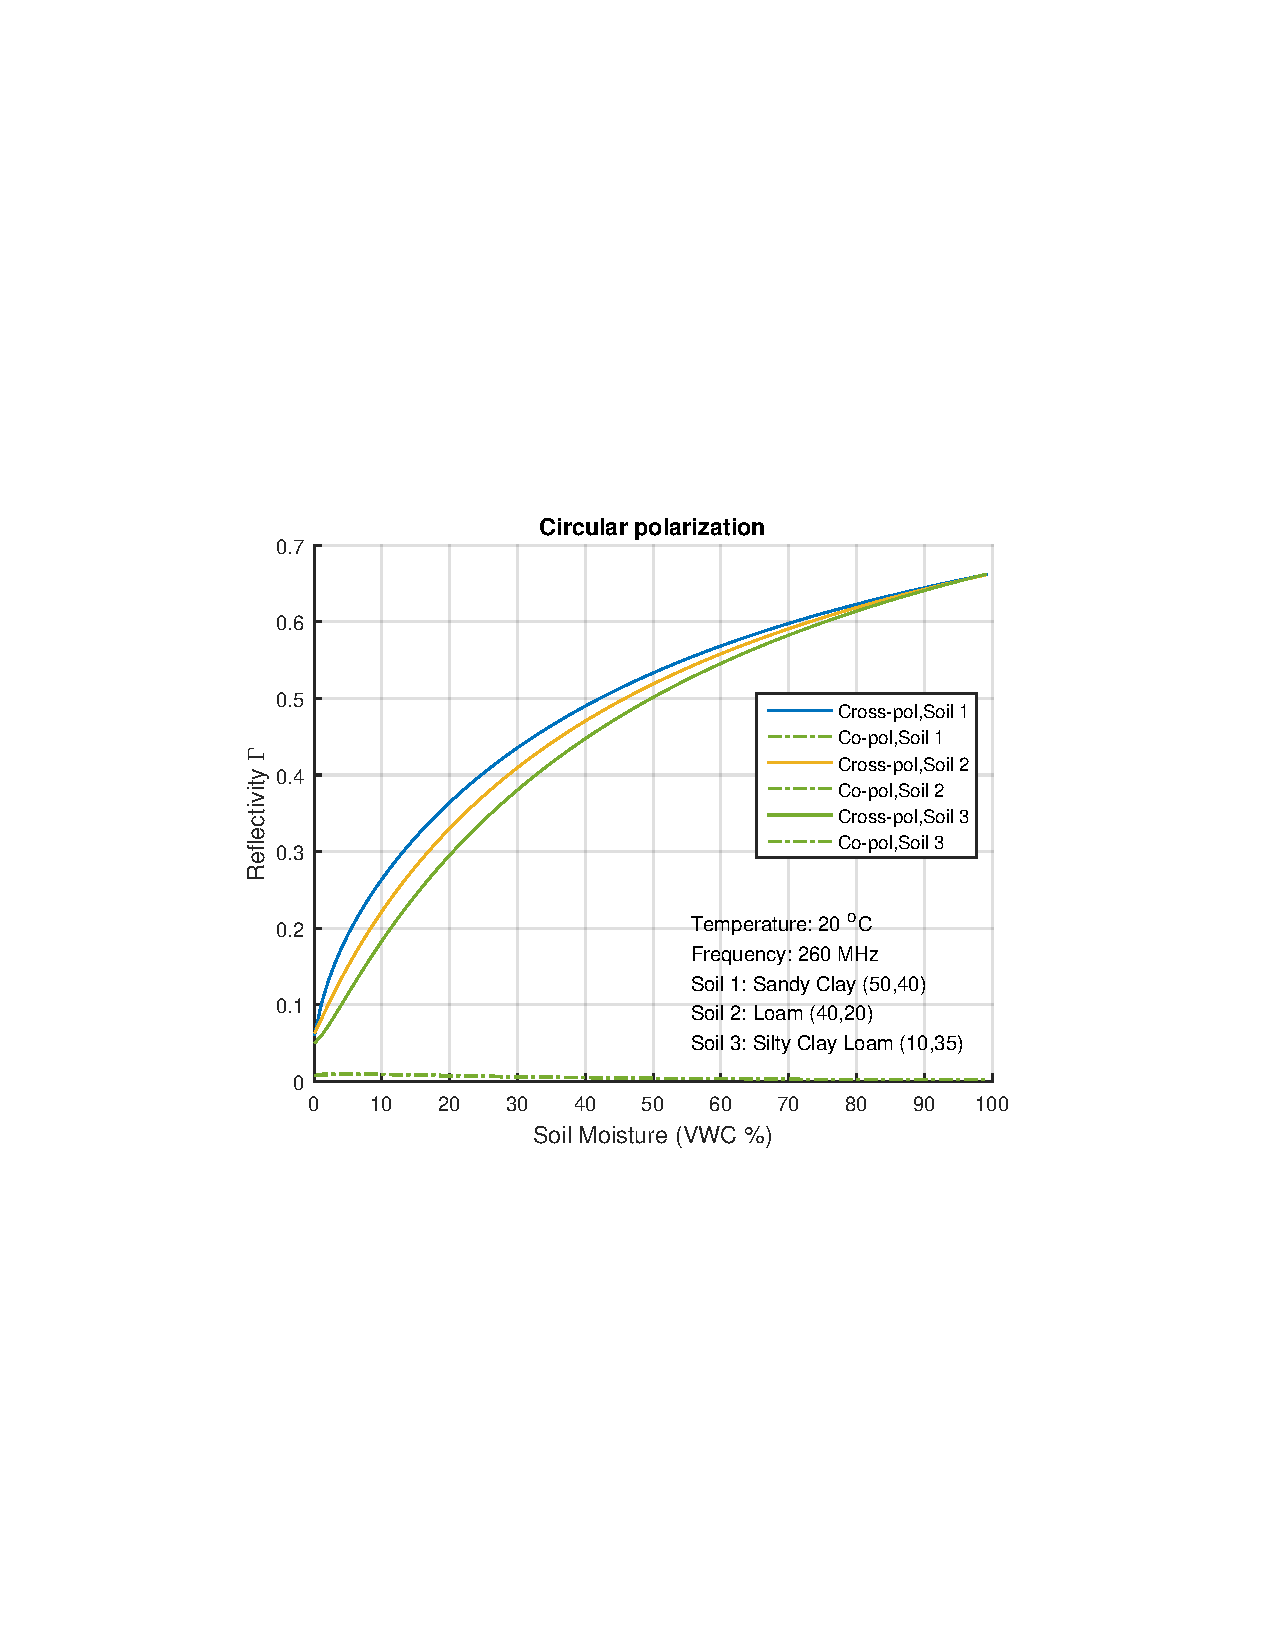
\includegraphics[width=6.5in]{pdf/gamma_vs_mv3.pdf}
	\caption{The reflectivity vs. soil moisture VWC($\%$) for the circular polarization with different soil types, 260 MHz frequency, and 20 $^\circ C$ temperature}
	\centering
	\label{fig:reflectivity}
\end{figure}
In figure \ref{fig:reflectivity}, the soil textures  of soil 1 to 3 are  (50,40), (40,20), and (10,35) for the percentile of sand and clay, and they are plotted in blue, yellow, and green, respectively. The solid line is cross-polarization, and the dash line is co-polarization.


These classical principles assume a perfectly flat interface between the air and a semi-infinite, uniform medium below the surface.
The limitations of the flat-surface interface can be approximated through the Rayleigh criterion on surface roughness. 
\begin{equation} 
  \sigma_z \leq \frac{\lambda}{8 \cos \theta}
     \label{Eq:rayleigh}
 \end{equation}
 For P-band (250~MHz), the wavelength is 1.2~m and so we can expect to assume specular reflection for a surface roughness up to 15~cm at the equator ($\theta = 0$) and 19~cm for mid-latitudes ($\theta = 40$ deg.). 
 In contrast, these limits are 2.3-3.1~cm at L-band (1.6~MHz) and 1.6-2.0~cm at S-band (2.3~GHz). 
 This long wavelength justifies our assumption of a specular refelction at P-band.
The more stringent Fraunhofer condition \cite{Ulaby:1981} will be met for soil roughness smaller than 5 cm. \bf I NEED TO LOOK THIS UP \rm.
  Experience with GNSS on TDS-1 \cite{Chew2016} showed coherent signals 92 \% of time with  GNSS-R (1.575~GHz). 
  Effects of roughness can be corrected through adjusting the reflectivity \cite{beckmann1987scattering}.
 \begin{equation} 
\Gamma_{pq} = \Gamma^S_{pq} \exp \left( - \beta \cos^2 \theta \right)
     \label{Eq:roughness}
 \end{equation}
 where $\beta$ is a ``roughness parameter'', given theoretically as $\beta =4 k^2 \sigma_z^2$ \cite{Choudhury2008}.
 
 Under the assumption of a specular reflection, the scattered signal will be coherent and thus the surface resolution from an altitude $h$ 
 will be set by the semi-major axis of the first Fresnel zone,  $a=\sqrt{\lambda h  \cos \theta}$, or 
 105~m from an aircraft altitude of 3~km and 1.5~km from a satellite in a 600~km orbit (assuming $\theta = 40$ deg.).



% penetration depth
This relationship will be the fundamental approach to sensing the soil moisture content within approximately the top layers of soil down to the penetration depth given in figure \ref{fig:depth}. The Penetration depth depth within an absorbing homogeneous material, in which the flux  of the field decays to $\frac{1}{e}$ of its surface value \cite{Ulaby:1981}.  This can be shown to be dependent on the imaginary part of the soil dielectric constant and the wavelength $\lambda$.
\begin{equation}
  \delta_p  = \frac{\pi}{\lambda} Im(\sqrt{\tilde{\varepsilon}_{r}})
\end{equation}
Where  $\alpha$ attenuation constant. Figure \ref{fig:depth} plots the penetration depth as a function of volumetric soil moisture, computed using the model \cite{Peplinski:1995}, for three frequencies, representing P-band (260 MHz), L-band(1.57542 GHz) and S-band (2.342205 GHz). Although the situation in a realistic  natural environment will be more complicated, with a heterogeneous multi-layer soil, and variable soil moisture profile, this simple definition of penetration depth will be used as an approximation of the soil depth to which microwave remote sensing is capable of making a measurement.  Figure \ref{fig:depth} clearly shows that measurements below the top few cm. of soil will require observations in P-band and lower frequencies. 
\begin{figure}[!t]
	\centering
	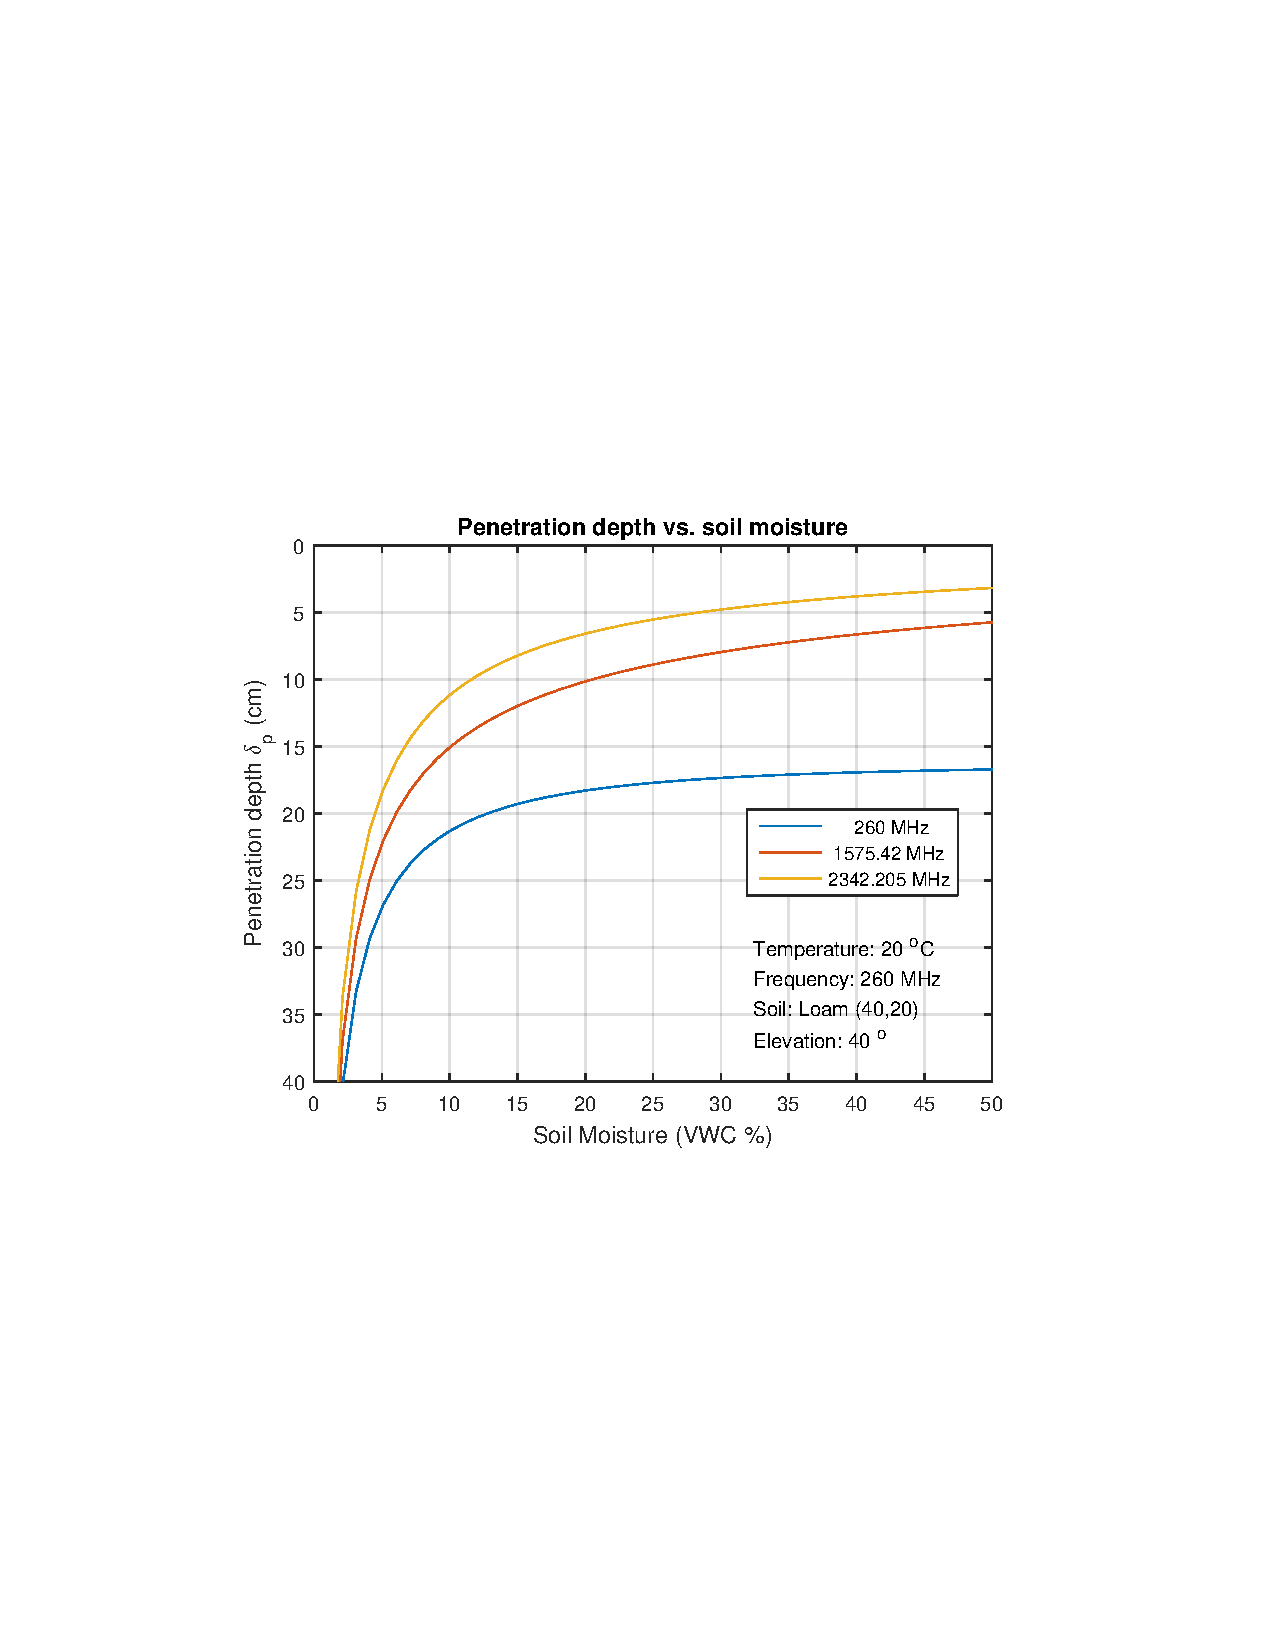
\includegraphics[width=6.5in]{pdf/penetration_depth.pdf}
	\caption{Penetration depth with different frequencies, 20 $^\circ C$ temperature, and soil texture (40, 20); blue, red, and yellow lines shows the penetration depth with 260 MHz, 1.57542 GHz, and 2.342205 GHz, respectively.}
   \centering
	\label{fig:depth}
\end{figure}


% Outline of rest of paper. 
%%%%
In this paper, we will present the essential design of an instrument for this measurement, using reflections of P-band signals of opportunity (SoOp) to estimate the surface reflectivity $\Gamma$. 
An approach to estimating the soil reflectivity through cross-correlating the reflected signal with the direct one will be developed in section \ref{section:Algorithm}.  Inverse methods to estimate the water distribution throughout a soil column from these measurements are beyond the scope of the work in this paper.  





The transmitted signal from a satellite ($x_{T}$) is modeled as
\begin{equation}
	x_T(t)=\sqrt{C_T}a(t)e^{j\omega_et},
    \label{Eq:xT}
\end{equation}
where $a(t)$ is the baseband digital signal.  The received signals at the object with antenna along the direct and reflected path ray can be represented 
\begin{eqnarray}
	%\begin{split}
  	x_D(t)&=\sqrt{C_D}a(t-\tau_D)e^{j\omega_e(t-\tau_D)}, \\
    x_R(t)&=\sqrt{C_R}a(t-\tau_R)e^{j\omega_e(t-\tau_R)}, 
   % \end{split}
    \label{Eq:xD_xR}
\end{eqnarray}
where $C_D$ and $C_R$ are received powers of signals the direct and reflected path at the antennas.  
$\tau_D$ and $\tau_R$ are the path delay along the direct and reflected path. The reflectivity $\Gamma$ is contained within the ratio of the direct and reflected powers
\begin{equation}
	\Gamma=\frac{C_{R}}{C_{D}}
    \label{Eq:reflect}
\end{equation}
Although a straighforward principle, the implementation of an instrument to extract this information introduces some complications.  
Specifically, the SoOp receiver must perform the following key functions to get to the reflectivity as defined in \ref{Eq:reflect}: 1.) isolate the signal $x_R(t)$ from $x_D(t)$, 2.) Remove the modulation $a(t)$ containing the data, and 3.) Remove effects of the antenna and receiver gains, and system noise.  
The next section will define the instrument design, and explain these functions in principle.  
The following section (\ref{sec:algorithm}) will develop the theory supporting this design and the algorithm to extract reflectivity. 
Finally, section (\ref{sec:error}) presents a simulation and error analysis. 


\section{Instrument Design}

[Jeff P, Manuel V]
\label{sec:instrument}
JLG: Do we want this here ? or after the theory section ? My view is give a general overview and then provide the numbers developed in the theory. 

\subsection{Requirements}

Host on B-200 or similar aircraft

Observation of geostationary transmitters operating between XXX and XXX deg. Elevation, transmitting between 230 and 270 MHZ, with bandwidth of 5-25 KHz, separated by XXX KHz. [give general overview here, but state the key assumptions about the transmitted source which drives the design process]  A detailed description of the signal source is provided in \ref{app:signal_source}

Working requirement for end-to-end retrieval accuracy of 0.04 volumetric water content.

Precision for altitude and attitude, which map through antenna gain. 

Table \ref{tab:sysreq} summarizes the system requirements derived from the science requirements [ jlg do we want to break these down so that you can show the flow-down ? or just state the key driving requirements]

Error analysis in \ref{sec:error} will show that these working requirements are expected to produce a system meeting the retrieval precision requirements. 

\begin{table}
\label{tab:sysreq}
\caption{System Requirements}
\begin{tabular}{|c|c|c|}
\hline
Parameter &  Value & Units \\
\hline
VMC Retrieval Precision &  0.04 & $m^3/m^3$ \\
\hline
Altitude precision &  100 & m \\
\hline
Attitude precision & 0.1 & deg \\
\hline 
Antenna Gain Knowledge & 0.2 & dB \\
\hline 
\end{tabular}

\end{table}

A summary of the complete system is shown in figure \ref{fig:schematic}.  It consists of a pair of two dual-pol antennas elements, identified as ``A'' and ``B'', connected to two parallel and independent analog sections, identified as ``1'' and ``2''  through a transfer switch.  The transfer switch will enable calibration of the receiver gain variations.  An antenna beam forming technique (described in \ref{sec:antenna}) will combined signals A and B to form a sky-view (S) and Earth-view (E) beam.  
The design requirement for this is to focus the S beam in the direction of the direct (D) line of sight signal with a null in the direction of the reflected (R) signal. 

\begin{figure}
	\centering
	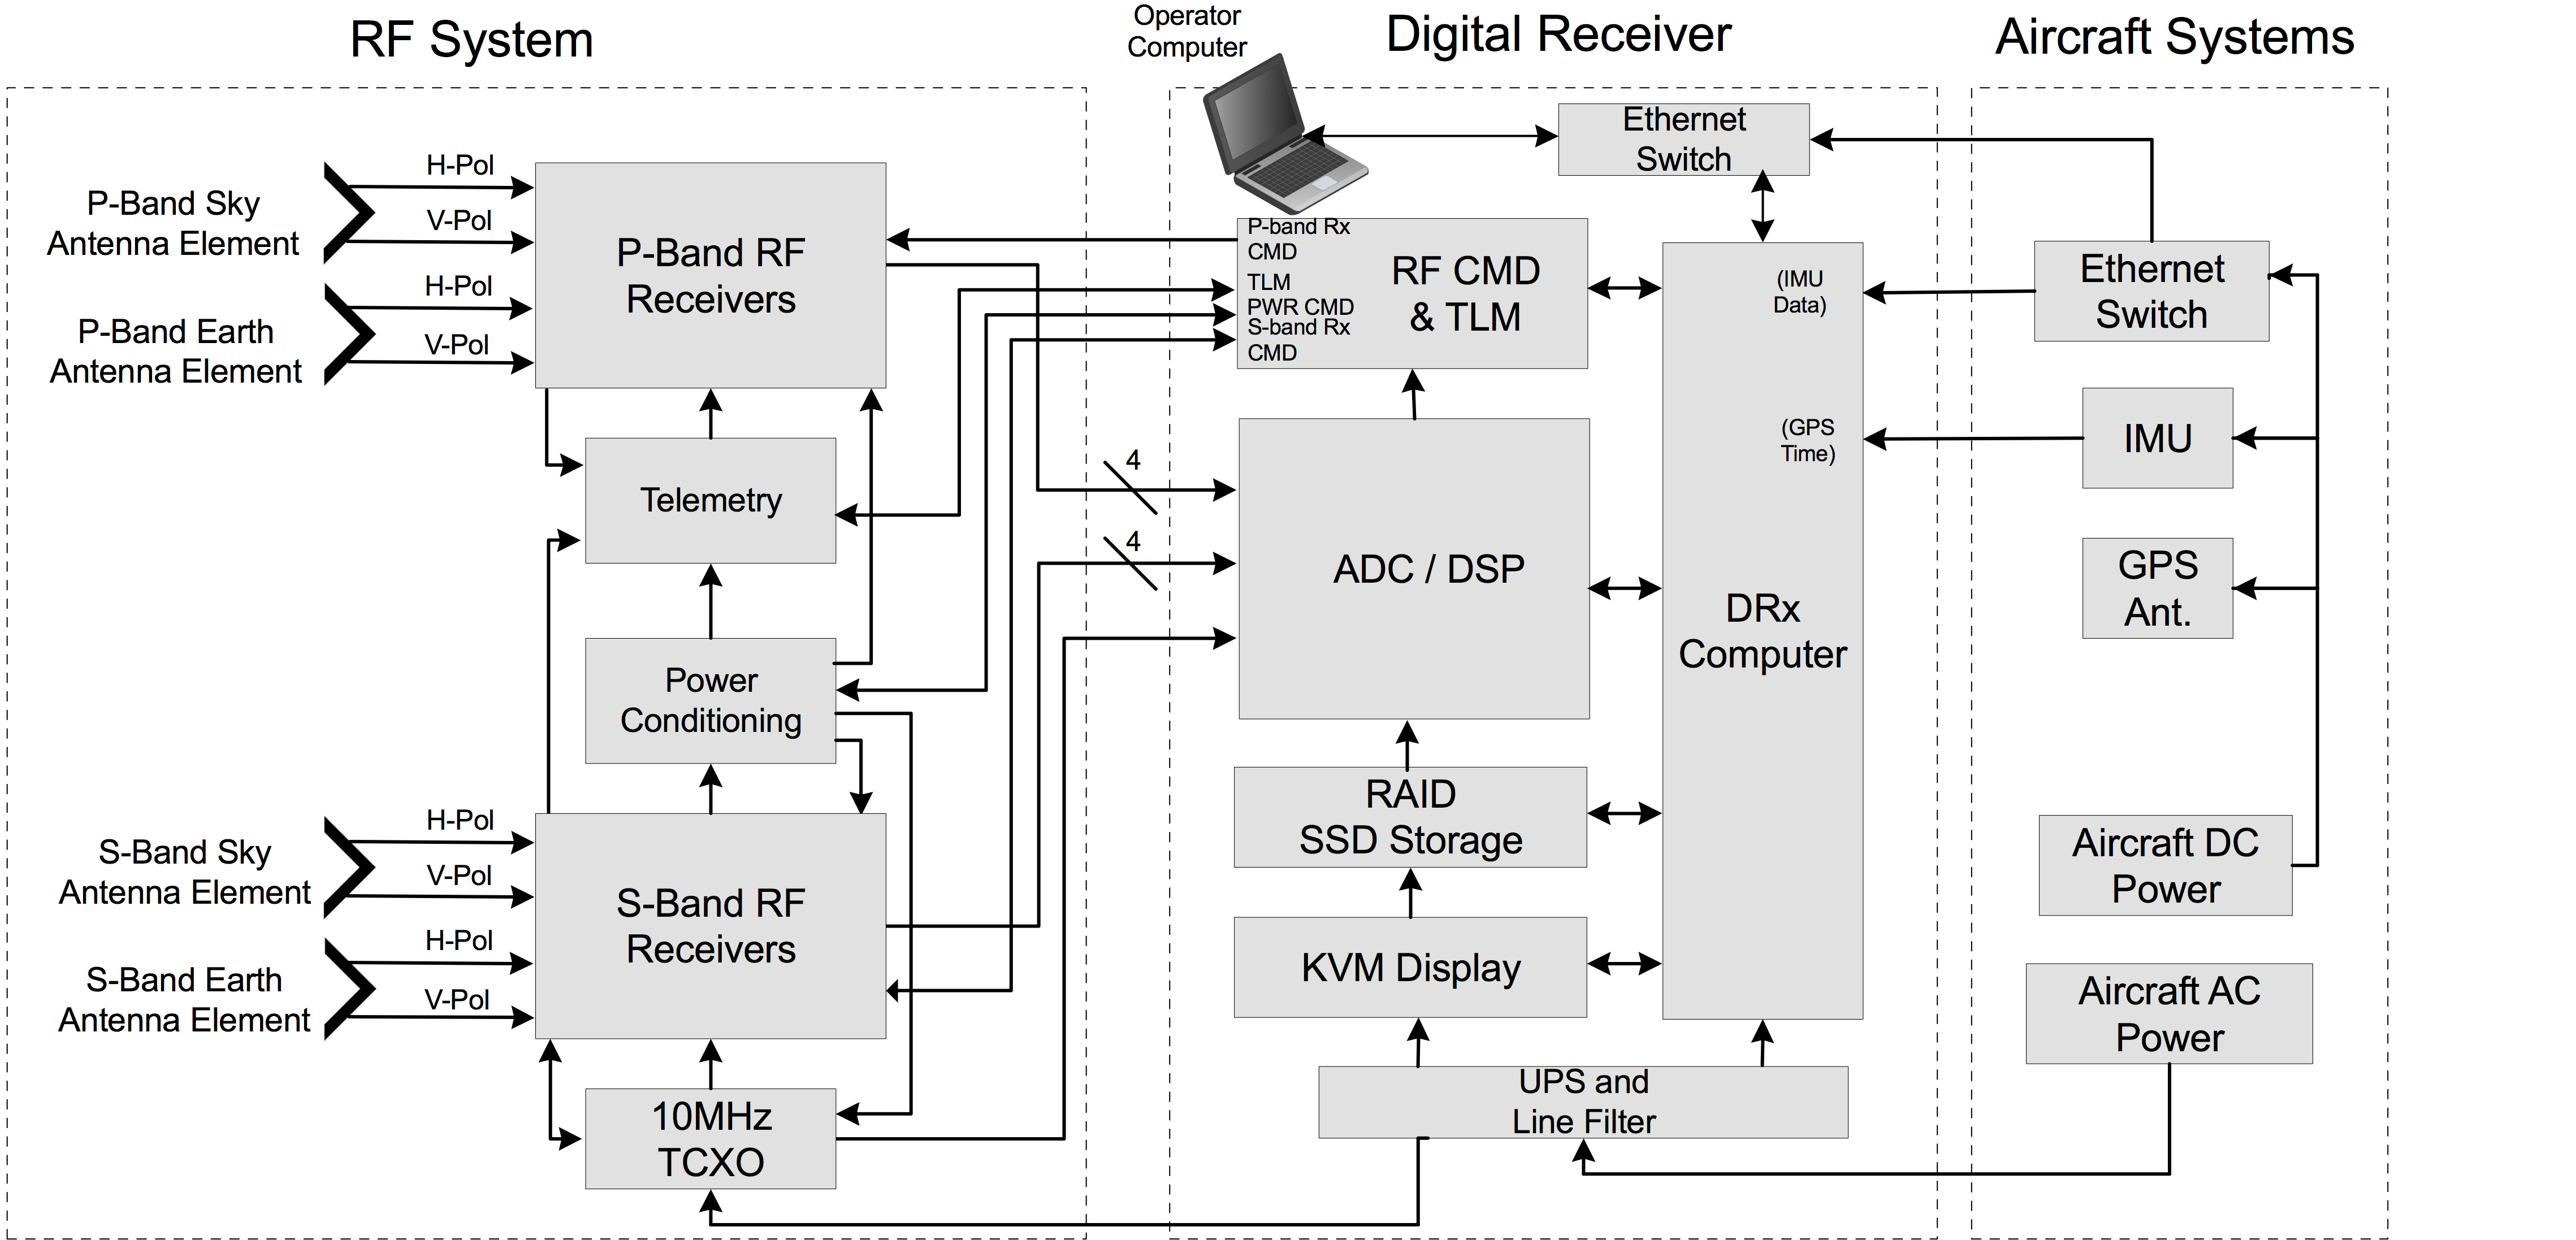
\includegraphics[width=4in]{pdf/SoOp_System_Architecture_Block_Diagram_04-03-17.png}
	\caption{SoOp-AD system architecture.}
   	\centering
	\label{fig:sysArch}
\end{figure}

Similarly, the E beam will be formed to have a maximum gain in the R signal direction, with a null in the D signal direction.
This beam-forming is not perfect, and quantifying the residual signal from R and D arriving in the S and E beams, respectively, will form an important part of the system error budget, developed in section \ref{sec:error}. 
Additional capability for calibration is provided by a calibrated thermal noise source.
A digital section will cross-correlate the the signals from receivers 1 and 2, at various fixed lags, to generate an array of complex cross-correlation values, which form the instrument or Level 0 data products.


Although assumed identical in design, the two receivers have different gains, $G_1$ and $G_2$, and different noise figures, both of which must be calibrated using a process described in section \ref{sec:calibration}.  
A transfer switch, which changes the connections between the antennas $\{ E, S \}$ and the receiver channels, $\{ 1, 2\}$ and noise sources are used for the calibration process. 


Technical details of these sub-systems are described below. 

\subsection{Antenna}
\label{sec:antenna}
[Nelis]

\bf JLG - I will incldue some description of the geometry - where the required lines of sight vary with latitude - must fly in a direction perpendicular to the scattering plane,  etc ... I generated a figure like this a while ago, will try to find it \rm 

SoOp ideally requires two antennas, where one antenna is a space view antenna isolated from the ground reflection, while the other is an earth view antenna isolated from the direct satellite signal.  Due to the low operating frequency, large high gain arrays are impractical for mounting on an aircraft.  Low single element antennas on the other hand cannot be isolated from certain signal directions just by virtue of their geometrical placement on the aircraft, as the latter is simply too small to provide effective shadow regions for each antenna.  Therefore the only option with two single element antennas is use electronic null-steering, which requires them to be mounted as close as possible to each other for maximum null width.  
The P-band antenna designed for SoOp consists of a two-element dual linearly polarized array, with an operating frequency of 255MHz and 40MHz bandwidth.  For mounting on the side of an aircraft, a low profile patch antenna geometry was chosen, with the distance between the elements limited to about 0.41 wavelengths.  The bandwidth requirement together with narrow spacing eventually lead to an element profile height of about 127mm.  To hug the aircraft as close as possible, the two elements are mounted with slightly differently tilted boresights, as shown in Fig???, while covered by an aerodynamical fairing/radome.  
The element design is based on an crossed-slot single patch-coupled geometry, with dual polarized excitation provided by two strip couplers above and below the slot’s crossing point as shown in Fig???.  Due to the large structure size, support of the various parts are provided by a light-weight rigid foam.  
Active S-parameters in a typical earth-view null-steering scenario is shown in Fig???, with the associated expected patterns shown in Fig???.  


\subsection{Analog Section}
\label{sec:analog}
[Manuel or Joe]

\subsection{Digital Section}
\label{sec:digital}

[Manuel or Joe ?]

\section{Measurement Theory}
 \label{section:Algorithm}

%
% JLG updates 3/6/2017
%
  Theory supporting the instrument conceptual design from section \ref{sec:instrument} is presented in this section. 
 First, the signal model at the input to the two digital receivers will be derived.
 This is followed by an expression for the general autocorrelation of each of these signals and the cross-correlation between them at multiple lags.  
 One important consideration is isolation between the direct and reflected signals.  
 In GNSS-R and other reflectometry measurements that use comparably wide-band transmissions, the short correlation length of the transmitted signal allows the use of cross-correlation for isolating the direct and reflected signals through  differences in delay. 
 Alternatively, the direct and reflected signals can be isolated through use of high-gain, narrow beam antennas [Ku band altimetry, P-band snow]. 
  P-band signals of opportunity, however, have narrow (25 KHz) bandwidths and a complete isolation between the direct and reflected signals will require a path length difference of at least 24~km. 
 Given the service ceiling of the B-200 aircraft is 10.7~km and assuming 
  a typical satellite elevation around $40^o$, the maximum path length difference will only be 15.1~km, thus presenting a mix of direct and reflected signal at both antennas. 
 The antenna design presented in section~\ref{sec:antenna} is capable of increasing isolation between the two signals by steering a null to the direction of the undesired signal. 
 Null-steering is limited by practical antenna design decisions, such as available space on the aircraft and the large patch size require for operating in P-band, however. 
 There will also be uncertainty in the gain pattern and the aircraft attitude dynamics.
 For these reasons, the retrieval algorithm is required to account for the interference between direct and reflected signals.  The algorithm should also be robust to uncertainty in the receiver gains, noise floor and aircraft altitude, all of which will be included in the error budget in section \ref{sec:error}.

 
 
\subsection{Signal Model}
The  signal $x_{T}$, transmitted from a satellite is modeled as
\begin{equation}
	x_T(t)=\sqrt{C_T}a(t)e^{j\omega_et},
    \label{Eq:xT}
\end{equation}
where  $C_{T}$ is the transmitted carrier power and $\omega_{c}$ is the  carrier frequency. %and $T_c$  is the chip period. 
$a(t)$ is  the baseband data signal, which has  a known autocorrelation  function, $R_a(\gamma)$. 
%and $p$ is an uniform distribution  on integers 0, 1, 2, 3, and rect denotes a rectangle function. 
Signals received at the aircraft antenna   along the direct, $x_D(t)$, and reflected, $x_R(t)$,  ray paths are given by 
\begin{eqnarray}
	%\begin{split}
  	x_D(t)&=\sqrt{C_D}a(t-\tau_D)e^{j\omega_c (t-\tau_D)}, \\
    x_R(t)&=\sqrt{C_R}a(t-\tau_R)e^{j\omega_c (t-\tau_R)}, 
   % \end{split}
    \label{Eq:xD_xR}
\end{eqnarray}
 $C_D$ and $C_R$ are  powers of signals the direct and reflected signals at the antenna location.  
$\tau_D$ and $\tau_R$ are the  delays along the direct and reflected paths. 
The reflectivity $\Gamma$ is defined as
\begin{equation}
	\Gamma=\frac{C_{RS}}{C_{DS}}
    \label{Eq:reflect}
\end{equation}
Where $C_{DS}$ and $C_{RS}$ are, respectively, the incident (direct) and reflected signal powers at the surface. 
We will define  the reflectivity measured  at the antenna by 
\begin{equation}
\Gamma_a = \frac{C_R}{C_D} = \frac{L_D C_{DS}} {L_R C_{RS}}
\end{equation}
Our algorithm  retrieves $\Gamma_a$,  $\Gamma$ can then be found from applying a link budget to estimate the path ``losses''  ( the aircraft is closer to the transmitter than to the surface, so $L_D > 1$ ). 
%between the surface and the aircraft, 
Given the low altitude, we will assume these losses are small and approximate $C_{DS}\approx C_D$ and $C_{RS}\approx C_R$. 
It would be straightforward to develop a link budget and correct this result for an improved estimate of surface reflectivity. 
%For an airborne receiver,  these losses can 
\begin{figure}[t!]
	\centering
    \centering
	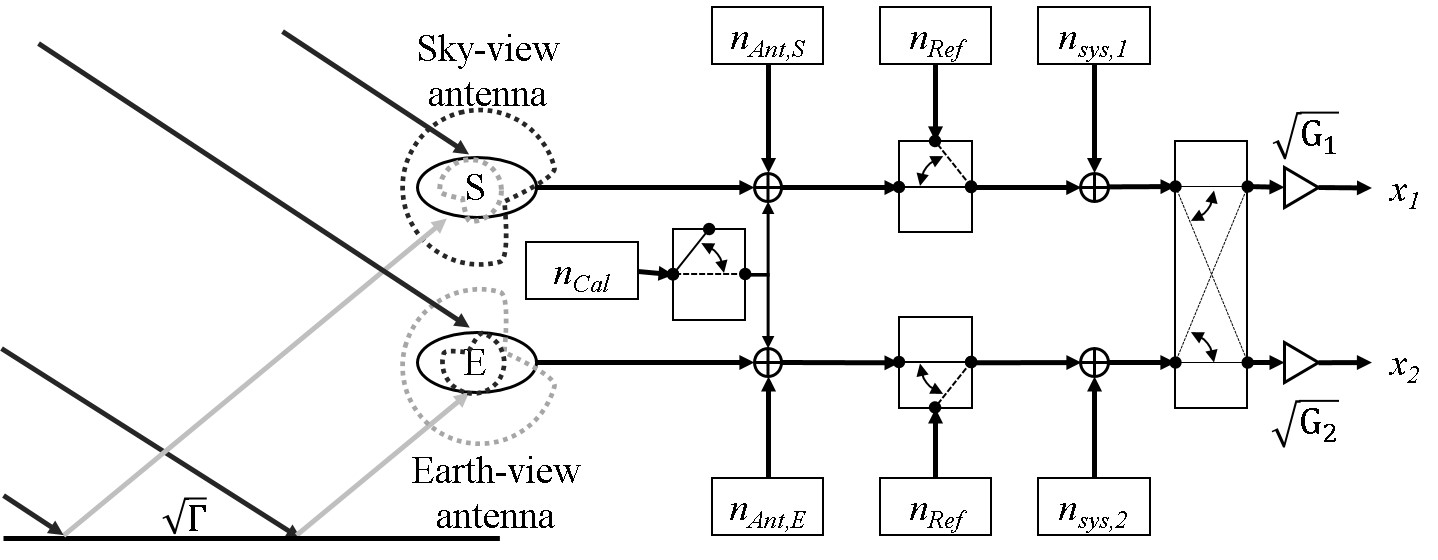
\includegraphics[width=5 in]{pdf/flow_chart_combine.jpg}
	\caption{The gain of sky-view and earth-view antenna for the direct and reflected path rays.. \bf ZENKI - combine with old fig 5 \rm}
	\label{fig:Hardware}
\end{figure}
Following the signal processing path  in Figure \ref{fig:Hardware}, the direct (D) and reflected (R) rays are each received by the sky-view (S) and Earth-view (E) antennas. 
 $G_{S,D}$ and $G_{S,R}$ are the gains of sky-view antenna gain along the direct and reflected path ray, respectively. 
 $G_{E,D}$ and $G_{E,R}$ are the gain of earth-view antenna gain along the direct and reflected path ray, respectively. 
 The antenna gain matrix  $\mathbf{G}_A = \mathrm{diag} [ \sqrt{G_{S,D}}, \sqrt{G_{E,R}}]$ contains the  line-of-sight gains. 
 Although the antenna null-steering will attempt to minimize $G_{E,D}$ and $G_{S,R}$, these gains cannot be assumed to be zero, and this is represented by the 
  isolation terms
\begin{equation}
    I_S  = \frac{G_{SR}}{G_{SD}},  \,\,\,\,
   I_E = \frac{G_{ED}}{G_{ER}}
\end{equation}
$G_1$ and $G_2$ are the gains of receiver channels 1 and 2, included in the receiver gain matrix $\mathbf{G}_R = \mathrm{diag} [ \sqrt{G_{1}}, \sqrt{G_{2}}]$
The transfer switch, defined by the matrix $\mathbf{T}_X$ alternates between the ``thru'' (T)  state and the ``swap'' (S) state. 
\begin{equation}
\mathbf{T}^T_X = \left[ \begin{array}{cc} 1 &  0 \\ 0 & 1 \end{array} \right] \,\,\,\,\,\,\,
 \mathbf{T}^S_X = \left[ \begin{array}{cc} 0 &  1 \\ 1 & 0 \end{array} \right]
\end{equation}
$n_{post,1}(t)$ and $n_{post,2}(t)$ are the noise sources in receivers 1 and 2  after (``post'')  the transfer switch and 
$n_{pre,S}(t)$ and $n_{pre,E}(t)$ are the noise from the antenna and the signal chain before (``pre'') the transfer switch. 
All noise is assumed to be zero-mean, band-limited, Gaussian processes with corresponding power-spectral densities $W_1$, $W_2$, $W_S$ and $W_E$.
Noise bandwidth, $B_N$, is assumed to be set by the anti-aliasing filter (equal to the sample rate). 
A single calibration noise, $n_{cal}(t)$, is injected into both signal chains, during the noise calibration described in section \ref{ssec:cal}, represented by setting 
$\mathbf{T}_c = [\begin{array}{cc} 1 & 1 \end{array} ]^T$. 
Receiver signals 1 and 2 are down-converted to an intermediate frequency, and then digitally downconverted to baseband. [The P-band receiver samples the 255 MHz directly without analog downconversion. MAV]
In our model, this downconversion will be assumed to have very small error.  \bf any reference to this in the error budget ? \rm
%$\omega_{IF} = \omega_c - \omega_{LO}$, using a local oscillator with  frequency $\omega_{LO}$. 
Signals $x_1(t)$ and $x_2(t)$, at the input to the A/D converters are given by
%\begin{equation}
%\left[ \begin{array}{c} x_1(t) \\ x_2(t) \end{array} \right] =  \sqrt{C_D}e^{j \omega_{IF} t}
 %  \left[ \begin{array}{cc} \sqrt{G_1} & 0 \\ 0 & \sqrt{G_2} \end{array} \right] \mathbf{T} 
  %    \left[ \begin{array}{cc} \sqrt{G_{S,D}} &  \sqrt{G_{S,R}} \\ \sqrt{G_{E,D}} & \sqrt{G_{E,R}} \end{array} \right] 
  %    \left[ \begin{array}{c} a(t-\tau_D) e^{-j \omega_c \tau_D} \\ \sqrt{\Gamma} a(t-\tau_R) e^{-j \omega_c \tau_R} \end{array} \right] + 
  % \left[ \begin{array}{c} n_1(t) \\ n_2(t) \end{array} \right]  
  % \end{equation}
   \begin{equation}
   \begin{split}
      \left[ \begin{array}{c} x_1(t) \\ x_2(t) \end{array} \right]  = &  \sqrt{C_D}e^{j \omega_{IF} t} \mathbf{G}_R \mathbf{T}_x \mathbf{G}_A
          \left[  \begin{array}{cc} 1  & \sqrt{I_S} \\ \sqrt{I_E} & 1  \end{array} \right]
           \left[ \begin{array}{c} a(t-\tau_D) e^{-j \omega_c \tau_D} \\ \sqrt{\Gamma_a} a(t-\tau_R) e^{-j \omega_c \tau_R} \end{array} \right] + ...\\
           ... & \mathbf{G}_R
           \left[ \begin{array}{c} n_{post,1}(t) \\ n_{post,2}(t) \end{array} \right]  + 
                      \mathbf{G}_R \mathbf{T}_x
           \left[ \begin{array}{c} n_{pre,S}(t) \\ n_{pre,E}(t) \end{array} \right]  
           + \mathbf{T}_c n_{cal}(t)
\end{split}
   \label{Eq: x2_model}
\end{equation}
%\begin{align}
 %	x_1(t)&= \sqrt{G_1} \left[ 
    %   \sqrt{G_{S,D} C_D} a(t-\tau_{D}) e^{-\omega_{IF} \tau_D} + 
   %    \sqrt{G_{S,R} C_R} a(t-\tau_{R}) e^{-\omega_{IF} \tau_R} 
    %  \right] + n_1(t)  \label{Eq: x1_model} \\ 
    %x_2(t)&=\sqrt{G_2}\left[ 
      %   \sqrt{G_{E,D} C_D}  a(t-\tau_{D}) e^{-\omega_{IF} \tau_D} + 
       %  \sqrt{G_{E,R} C_R} a(t-\tau_{R}) e^{-\omega_{IF} \tau_R}\right] + n_2(t) 
 % \label{Eq: x2_model}
%\end{align}

A second calibration state, identified as  ``reference'' (R),  is performed when receiver 1 and 2 are switched to reference loads, with noise processes $n_{ref,1}(t)$ and $n_{ref,2}(t)$. 
This is only performed with the transfer switch in the T state. 
In the R-state, the signal at the receivers will be  
  \begin{equation}
      \left[ \begin{array}{c} x^{R}_1(t) \\ x^{R}_2(t) \end{array} \right]  =  
           \mathbf{G}_R
           \left[ \begin{array}{c} n_{post,1}(t) + n_{ref,1}(t)  \\ n_{post,2}(t)  + n_{ref,2}(t) \end{array} \right]  
%                      \mathbf{G}_R \mathbf{T}_S
  %         \left[ \begin{array}{c} n_{pre,S}(t) \\  \end{array} \right]  
     %      + \mathbf{T}_c n_{cal}(t)
           \label{Eq:x2_ref_state}
\end{equation}
\subsection{Correlation}
The digital receiver  performs a finite-time cross-correlation between two signals ($x_p$ and $x_q$) at delay $\tau$, using an integration time $T_I$. 
\begin{equation}
	Y_{pq}(\tau)  %=\langle x_p^*(t)x_q(t+\tau)\rangle
    =\frac{1}{T_I} \int_{T_I}x_p(t) x_q^*(t+\tau)dt 
   % R_{pq}(\tau-\tau_{qp}) =\langle x_p^*(t-\tau_p)x_q(t-\tau_q +\tau)\rangle
    \label{Eq:correlation_def}
\end{equation}
We will assume $T_I$ is sufficiently long and that modulation is generated from an infinitely-long, constant envelope digital signal, so that the autocorrelation of $a(t)$ is approximately given by
\begin{equation}
R_a (\tau) = \frac{1}{T_I} \int_{T_I} a(t) a^*(t+\tau) dt
\end{equation}
% known and has the following properties.
%\begin{align}
  % \label{eqn:acfa1}
%	R_{a}(0) &= 1   \\
  %  R_{a}(\tau) & = R_a^* (-\tau)
  %  \label{eqn:acfa2}
%\end{align}
If the modulation of $a(t)$ is known then $R_a(\tau)$ can be computed from a model.
It can also be measured experimentally through observation of the direct line-of-sight signal $x_D(t)$ with pair of directional antennas (described as the ``self-ambigiuty function'' in [Griffiths ... ]).  The latter procedure is described in Appendix \ref{App: Ra} and was applied to this problem. 
 The matrix of cross-correlations (\ref{Eq:correlation_def})  
 between channel 1 and 2, at a  delay, $\tau$, 
 \begin{equation}
 \mathbf{Y}(\tau) =  \left[ \begin{array}{cc}  Y_{1,1}(\tau) & Y_{1,2}(\tau) \\ Y_{2,1}(\tau) & Y_{2,2}(\tau)  \end{array} \right]
  \label{eqn:xcorrmatdefn}
 \end{equation}
 can be shown to be the following. 
  \begin{equation}
 \mathbf{Y}(\tau) = 
 C_D \mathbf{G}_R \mathbf{T}_X \mathbf{G}_A  \mathbf{F}(\Gamma_a, \phi, \tau_{RD}, I_E, I_E )
 \mathbf{G}_A^T \mathbf{T}_X \mathbf{G}_R^T + \mathbf{G}_R \left( \mathbf{N}_{sn}(\tau)   + \mathbf{N}_{nn}(\tau) \right)  \mathbf{G}_R^T
 \label{eqn:xcorrmat}
 \end{equation}
 The two unknowns, $\Gamma_a$ and $\phi=\omega_c \tau_{RD}$, appear only in the matrix $\mathbf{F}$. 
  \begin{equation}
 \mathbf{F}() =   \left[  \begin{array}{cc} 1  & \sqrt{I_S} \\ \sqrt{I_E} & 1  \end{array} \right]
 \left[ \begin{array}{cc} R_a(\tau) & \sqrt{\Gamma_a} R_a(\tau-\tau_{RD})  e^{j \phi }  \\ 
    \sqrt{\Gamma_a} R_a(\tau+\tau_{RD}) e^{-j \phi} & \Gamma_a R_a(\tau) \end{array} \right]
     \left[  \begin{array}{cc} 1  & \sqrt{I_S} \\ \sqrt{I_E} & 1  \end{array} \right]^T
 \label{eqn:fmat_defn}
 \end{equation}
$\mathbf{N}_{sn}(\tau)$  is matrix of zero mean random variables, resulting from the cross-correlation of signal with noise. 
The cross-correlation of noise with itself, $\mathbf{N}_{nn}(\tau)$,  has a non-zero mean (the ``noise floor'') which needs to be estimated and removed in order to accurately observe the reflectivity. 
% Where $\phi = \omega_c \tau_{RD}$ is the phase difference between the direct and reflected ray paths and
%\begin{equation}
%E \left\{ \mathbf{N}_{nn} (\tau)\right\} = 
%\left(   \left[ \begin{array} {cc} W_1 & 0 \\ 0 & W_2 \end{array} \right] + \mathbf{T}_x  \left[ \begin{array} {cc} W_S & 0 \\ 0 & W_E \end{array} \right] \mathbf{T}_x^T 
% +W_{cal}   \mathbf{T}_c   \mathbf{T}^T_c  \right) 
%    \left[ \begin{array} {cc}  B_N \mathrm{sinc} B_N \tau & 0  \\ 0 &  W_2 B_N \mathrm{sinc} B_N \tau \end{array} \right]
%\end{equation}
If the sample rate is assumed to be set equal to the Nyquist rate, then the smallest increment in delay will be $\Delta \tau \approx B_N^{-1}$ and 
will generate independent noise samples. 
In this case, 
%$E\{ \mathbf{N}_{nn}(\tau)\}  \approx \mathbf{0}$, for $\tau \neq 0$ and  
%$E\{ \mathbf{N}_2(0)\} =\mathrm{diag} [W_1 B_N,  W_2 B_N]$. 
the two noise terms are approximately give by
\begin{equation}
\mathbf{N}_{sn} (\tau) + \mathbf{N}_{nn} (\tau) = 
\left(   \left[ \begin{array} {cc} W_1 B_N & 0 \\ 0 & W_2 B_N \end{array} \right] + \mathbf{T}_x  \left[ \begin{array} {cc} W_S B_N& 0 \\ 0 & W_E B_N \end{array} \right] \mathbf{T}_x^T 
 +W_{cal}  B_N \mathbf{T}_c   \mathbf{T}^T_c  \right) 
 \Delta(\tau) + \tilde{\mathbf{n}}
%    \left[ \begin{array} {cc}  B_N \mathrm{sinc} B_N \tau & 0  \\ 0 &  W_2 B_N \mathrm{sinc} B_N \tau \end{array} \right]
\end{equation}
in which 
\begin{equation}
\Delta(\tau) = \left\{ \begin{array}{cc}  1, & \tau = 0 \\ 0, & | \tau | > 0  \end{array}\right.
\end{equation}
and $\tilde{\mathbf{n}}$ is a diagonal matrix, with zero-mean normally-distributed elements. 

% The receiver noise can be expressed as a single equivalent thermal noise source at the input of the receiver, with the following properties.
%\begin{equation}
%\begin{split}
%	R_a(\tau)&=\frac{1}{T_I} \int_{T_I}a(t) a^*(t+\tau)dt  \\
  %  R_a(\tau-\tau_{RD})&=\frac{1}{T_I} \int_{T_I}a(t-\tau_D) a^*(t-\tau_R+\tau)dt  \\
  %  R_a(\tau+\tau_{RD})&=\frac{1}{T_I} \int_{T_I}a(t-\tau_R) a^*(t-\tau_D+\tau)dt 
 %\end{split}
%\end{equation}

%The correlation of noise $n_1$ and $n_2$ are defined as
%\begin{equation}
%\begin{split}
  %  \frac{1}{T_I} \int_{T_I}n_1(t) n_1^*(t+\tau)dt  &=  \sigma_1^2 (R_n(\tau) + n_{RES})\\
%	\frac{1}{T_I} \int_{T_I}n_2(t) n_2^*(t+\tau)dt  &=  \sigma_2^2 (R_n(\tau) + n_{RES})\\
  %  \frac{1}{T_I} \int_{T_I}n_1(t) n_2^*(t+\tau)dt  &=  \sigma_1 \sigma_2  n_{RES}
% \end{split}
%\end{equation}


\subsection{Definition of a Reflectivity Observable}
 \label{sec: Observable and Forward Model}
We will define an observable from  a combination of elements of the correlation matrix in (\ref{eqn:xcorrmat}) at specific delays.
This observable can then be solved for  reflectivity, $\Gamma_a$, in the presence of  interference between the direct and reflected ray paths and uncertainty in aircraft altitude. 
%The ratio of receiver gains, $r_{1,2} =  \sqrt{G_1/G_2}$, will be determined by the antenna swapping, as described in section XXX. 
Antenna gains,  $G_{S,D}$, $G_{S,R}$, $G_{E,R}$, $G_{E,D}$,  first obtained from modeling and chamber tests, will be corrected during calibration flights (accounting for effects of aircraft integration) and can be   
%described in section \ref{sec:calibration} and 
%After calibration, antenna gains can be 
assumed to remain constant for a given aircraft installation. 
Receiver gains and the noise floors  can drift with time, however. 
%Antenna swapping [ref to AE] will be used to estimate the ratio $r_{1,2}$    with the  $\mathbf{T}_x$ matrix alternating between its two states with a 50\% duty cycle for each.
Switching to the R-state will provide independent estimates of $G_1$ and $G_2$.
Injection of noise in the calibration (C) state  and modeling of the antenna noise temperature will be used to estimate the channel 1 and 2 noise floors, 
$N_{11} = W_1 B_N + W_S B_N$ and $N_{22} = W_2 B_N + W_S B_N$.
These calibration processes are described in section \ref{ssec:cal}

To begin the derivation of an observable, first consider  ideal antennas providing perfect isolation between the direct and reflected signals, 
 $G_{S,R}\approx 0 $ and $G_{E,D}\approx 0$. 
and  a perfect downconversion to baseband, so that the immediate frequency $\omega_{IF} \approx 0$. 
\bf JLG - how importnat is this 2nd asusmption ? cross-correlation will remote most of the frequency error anyway - except a term of (freq error) * tau \rm
The following observable is formed from observations made in the T-state
%  incorporating  parameters from the calibration processes and elements of the correlation matrix (\ref{eqn:xcorrmat}) evaluated at $\tau=0$ and $\tau= \tau_{RD}$. 
\begin{eqnarray}
 \Gamma_o^T =	r_{12} \sqrt{\frac{G_{S,D}}{G_{E,R}}} \frac{Y_{12}^T(\tau_{RD})} {Y_{11}^T(0)-G_1 N_{11}}  
    \label{Eq:Gamma_estimation_approx}
% * <lin184@purdue.edu> 2017-03-07T06:34:19.198Z:
% 
% r_{12} or r_{1,2}?
% Y_{11) or Y_{1,1}
% 
% ^.
\end{eqnarray}
and an equivalent one is formed from observations made in the S-state
\begin{eqnarray}
 \Gamma_o^S =	r_{12} \sqrt{\frac{G_{S,D}}{G_{E,R}}} \frac{Y_{21}^S(\tau_{RD})} {Y_{22}^T(0)-G_1 N_{22}}  
    \label{Eq:Gamma_estimation_approx}
% * <lin184@purdue.edu> 2017-03-07T06:34:19.198Z:
% 
% r_{12} or r_{1,2}?
% Y_{11) or Y_{1,1}
% 
% ^.
\end{eqnarray}
% * <lin184@purdue.edu> 2017-03-07T16:32:47.761Z:
% 
% how is $G_1$ estimateEq:Gamma_estimation_approxd separately from $r_{1,2}$ ?
% 
% I did not estimate G1 directly. G1 can be estimated from noise injection. Check the calibration section
% 
% ^ <jlgarrison66@gmail.com> 2017-03-16T02:28:31.280Z.
%e Once these parameters, assumed to remain constant after calibration, are obtained, the following observable is formed. 

%Substitution of (\ref{Eq:R11}), (\ref{Eq:R22}), and (\ref{Eq:R12}) into
%(\ref{Eq:Gamma_estimation_approx}), with the assumptions that $G_{S,R}=0$, 
%$G_{E,D}=0$ and $R_a(0)=1$, results in
%\begin{equation}
%\Gamma_{12} = \sqrt{\frac{G_1}{G_2}} \sqrt{\frac{G_{S,D}}{G_{E,R}}} 
 % \frac{e^{-j \omega_c \tau_{RD}} g_{1SD} g_{2ER} +\sigma_1 \sigma_2 n_{RES}}
   %  {g_{1SD}^2 + \sigma_1^2 n_{RES}}
   %  \label{Eq:Gamma_estimation_approx_subst1}
%\end{equation}
%\approx\sqrt{\hat{\Gamma}}e^{j\omega_e \tau_{RD}} 
it is straightforward to show that both of these reduce to 
\begin{equation}
    \Gamma_{o} = \sqrt{\Gamma_a} e^{-j \phi} + n_\Gamma
    \label{Eq:Gamma_estimation_approx}
\end{equation}
under the assumption of a high signal to noise ratio (SNR). 
 $n_\Gamma$ is a zero-mean random variable. 
%Substituting (\ref{Eq:g1sd}) and (\ref{Eq:g2er}), with the high SNR assumption, reduces (\ref{Eq:Gamma_estimation_approx_subst1}) to 

If the antennas had perfect isolation,  $\Gamma_a$ could be determined simply by computing the magnitude of the observable $\Gamma_{o}$.
%defined in (\ref{Eq:Gamma_estimation_approx}). 
Precise knowledge (e.g. better than a wavelength) of the path delay, $\tau_{RD}$, is not required,  as this will be manifested as a rotation of $\Gamma_{o}$ in the complex plane, not in a change in the magnitude.   
Path delay will depend upon both the aircraft altitude and the terrain elevation. 
A value for $\tau_{RD}$ is necessary for the argument of $Y^T_{12}(\tau_{RD})$ or $Y^S_{21}(\tau_{RD})$, but  the required precision of this is much lower due to the  low bandwidth of P-band SoOp signals (25~KHz).
Sensitivity to $\tau_{RD}$ (and additional parameters) is studied in section \ref{sec:error}. 
An assumption that the altitude does not very substantially (more than a small fraction of a wavelength) during the integration time, $T_I$ is implicit in   these conclusions.
This will be evaluated  in section \ref{sec:altitude}.

%The  phase of $\Gamma_{1,2}$ will show a much grater sensitivity to the path delay, rotating  through one complete cycle for a 1.2~m change in altitude.  

Given the long wavelength of P-band signals and the practical limitations of designing an antenna for use on aircraft,  perfect isolation of the direct and reflected signals will not possible. 
When  the  gains $G_{S,R}$ and $G_{E,D}$ are not zero, the observable (\ref{Eq:Gamma_estimation_approx}) can still be written in the general form 
\begin{equation}
\Gamma_{o} = f(\Gamma_a, \phi) +n_{\Gamma}
  \label{eqn:observation_eqn_general}
\end{equation}
with a more complicated dependence on $\Gamma_a$ and $\phi$. 
\begin{equation}
f(\Gamma, \phi) =
	\frac{(\sqrt{I_E}+\sqrt{I_S}\Gamma_a)R_a(\tau_{RD})+\sqrt{\Gamma_a} 
    e^{j\phi}+\sqrt{I_S I_E\Gamma_a} R_a(2\tau_{RD})e^{-j\phi}} 
    {(1 + I_S \Gamma_a) + 2 \sqrt{I_S \Gamma_a} \mathrm{Re}\left\{ R_a(\tau_{RD}) e^{j \phi} \right\} }
        \label{Eq:Gamma_estimation}
\end{equation}
%An observable and forward model must be developed, which accounts for the interference between the direct and reflected signals, due to  In general, the $\Gamma_{12}$ observable can be written in the form of an observation equation as a function of two variable,s $\Gamma$ and the phase difference along the reflected ray path, $\phi = \omega_c \tau_{RD}$, with  additive noise.  $n_{\Gamma}$. 

%A full expression for $f(\Gamma, \phi)$, removing the assumption of perfect isolation, is given by

%
%                   {(1 + I_S)\Gamma)R_a(0)+2\sqrt{I_S\Gamma} R_a(\tau^s_{RD})cos\phi}  
%Equation (\ref{eqn:Gamma_estimation}) can solved numerically for $\Gamma_a$ and $\phi$. 

\subsection{Reflectivity Retrieval}  
\label{sec: Reflectivity Retrieval}
Equation (\ref{Eq:Gamma_estimation}), when plotted in the complex plane (figure \ref{fig:Gamma12}) shows the effect of the antenna isolation.  
This figure was generated using the preliminary system design parameters from table \ref{tab:sysparam}
and shows curves for the complex function $f(\Gamma, \phi) $,  plotted for  a range of  different reflectivities (stated in the caption). 
This  is overlaid on the perfect isolation example presented earlier, in which each of these curves is  a circle centered on the origin. 
$f(\Gamma, \phi)$ forms a closed curve over one cycle of the phase (about 1.2~m change in $\tau_{RD}$. % range of $-\pi \leq \phi \leq \pi$. 

[Review this figure caption. Black lines are for non-ideal isolation, right?  MAV]
\begin{figure}[t!]
	\centering
    \centering
	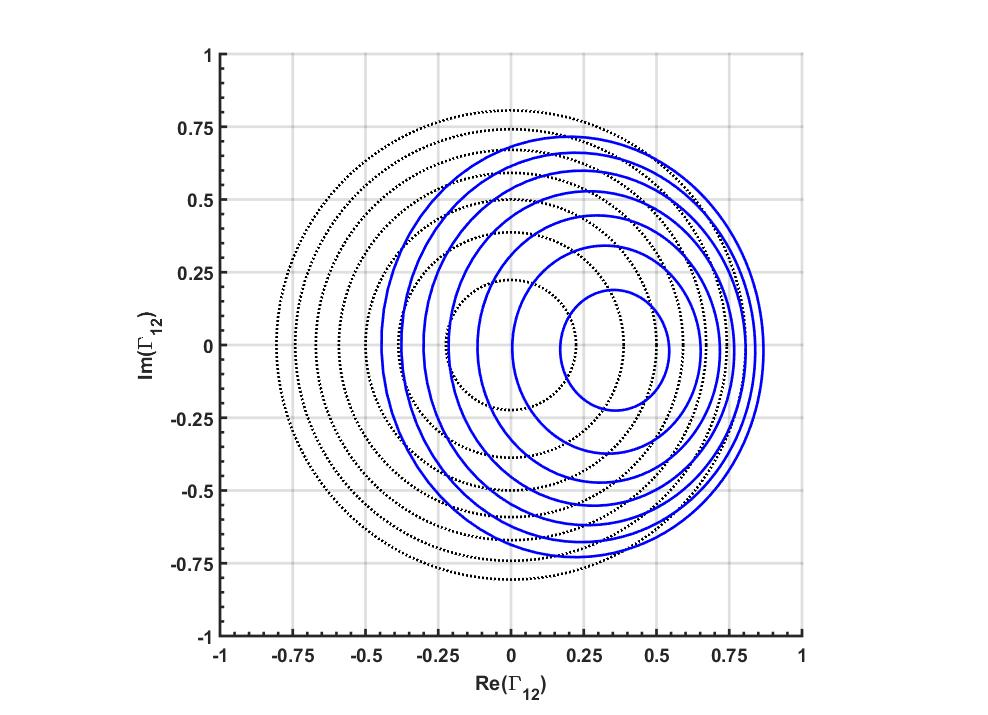
\includegraphics[width=5 in]{pdf/Gamma12.jpg}
	\caption{The complex plot of $\Gamma_{12}$ with and without ideal antenna isolation; the black dot lines represent $\Gamma_{12}$ with ideal antenna isolation, the blue lines are $\Gamma_{12}$ with ideal antenna isolation, and reflectivities are 0.05, 0.15, 0.25, 0.35, 0.45, 0.55, and 0.65 from inner to outer contours.}
	\label{fig:Gamma12}
\end{figure}

As can be seen, the effects of non-zero $I_E$ and $I_S$ are to transform this circle into an ellipse, and shift its center away from the origin. 
The important consideration, however, is that the curves for different reflectivities do not intersect and thus there is a unique mapping between the real and imaginary parts of the observable and model.  
Retrieval of a reflectivity estimate, $\hat{\Gamma}$ can therefore be found from the complex observable $\Gamma_{o}$ simply by numerical solution of the system of two (2) equations (real and imaginary parts) 
\begin{equation}
\Gamma_{o} - f(\hat{\Gamma}, \hat{\phi}) = 0
\label{eqn:2x2solution}
\end{equation}
$\hat{\phi}$ will be an auxiliary variable to account for  rotation in the complex plane due to the variations in path delay.  
As with the ideal case, this eliminates the need for high-precision knowledge of the aircraft altitude or terrain.  
Newton's method was found to work well for the solution of (\ref{eqn:2x2solution}). 

\begin{table}[ht]
\centering
\caption{System design specifications}
\begin{tabular}  {|c|c|c|c|}
	\hline
     \textbf{Parameter} & \textbf{Symbol}	& \textbf{Value} &	\textbf{units}  \\
     \hline
     Incident Direct Power &	$C_T$ & 14  & 	dBW	\\
          \hline
     Noise Power of channe 1&	 $\sigma_1^2$ & -131.0964  & 	dBW	\\
     \hline
      Noise Power of channel 2&	$\sigma_2^2$ & -130.2362  & 	dBW	\\
     \hline
     Gain of sky-view antenna along direct path ray &	$G_{S,D}$ & 6.7972  & 	dB	\\
    \hline
         Gain of earth-view antenna along reflected path ray&	$G_{SR}$ & 0.5123  & 	dB	\\
    \hline
         Gain of sky-view antenna along direct path ray &	$G_{ED}$ & 0.1192  & 	dB	\\
    \hline
             Gain of earth-view antenna along reflected path ray &	$G_{ER}$ & 4.9115  & 	dB	\\
    \hline
    Gain of channel 1 &	$G_1$ & 0  & 	dB	\\
    \hline
    Gain of channel 2 &	$G_2$ & 0  & 	dB	\\
    \hline
\end{tabular}
\label{tab:sysparam}
\end{table}

\section{Calibration}
\label{sec:calibration}
The reflectivity retrieval method described in the  previous section requires numerical values for 
seven parameters in addition to the cross-correlations. 
%in order to perform the retrieval of $\Gamma_a$  
These parameters are;
antenna gains in the direct and reflected ray path directions ($G_{S,D}$, $G_{S,R}$, $G_{E,D}$, $G_{E,R}$),  
channel gain ratio ($r_{1,2} = G_1/G_2$), and  two noise floors $N_{1,1}$ and $N_{2,2}$.
We will assume that the antenna gain patterns, properties of the antenna design and integration on the airframe,  will 
 remain constant. 
A companion paper, describing the antenna design and the in-flight calibration process, is being written.  
We will use the nominal values obtained from numerical simulation for these gains.
%as  given in table \ref{tab:sysparam}.
 Noise power and the receiver gains, however, are expected to vary with time and will need to be periodically calibrated. 
%Two approaches are used for this calibration; injection of noise sources (states C and R) and  antenna swapping (states T and S)  and 
Refer to the right side of figure \ref{fig:Hardware} for the architecture of calibration chain.
Configuration for the four operational states of the instrument; Thru (T), Swap (S), Calibration (C) and Reference (R), are  
 illustrated in figure \ref{fig:hw_states}
\begin{figure}[h]
	\centering
	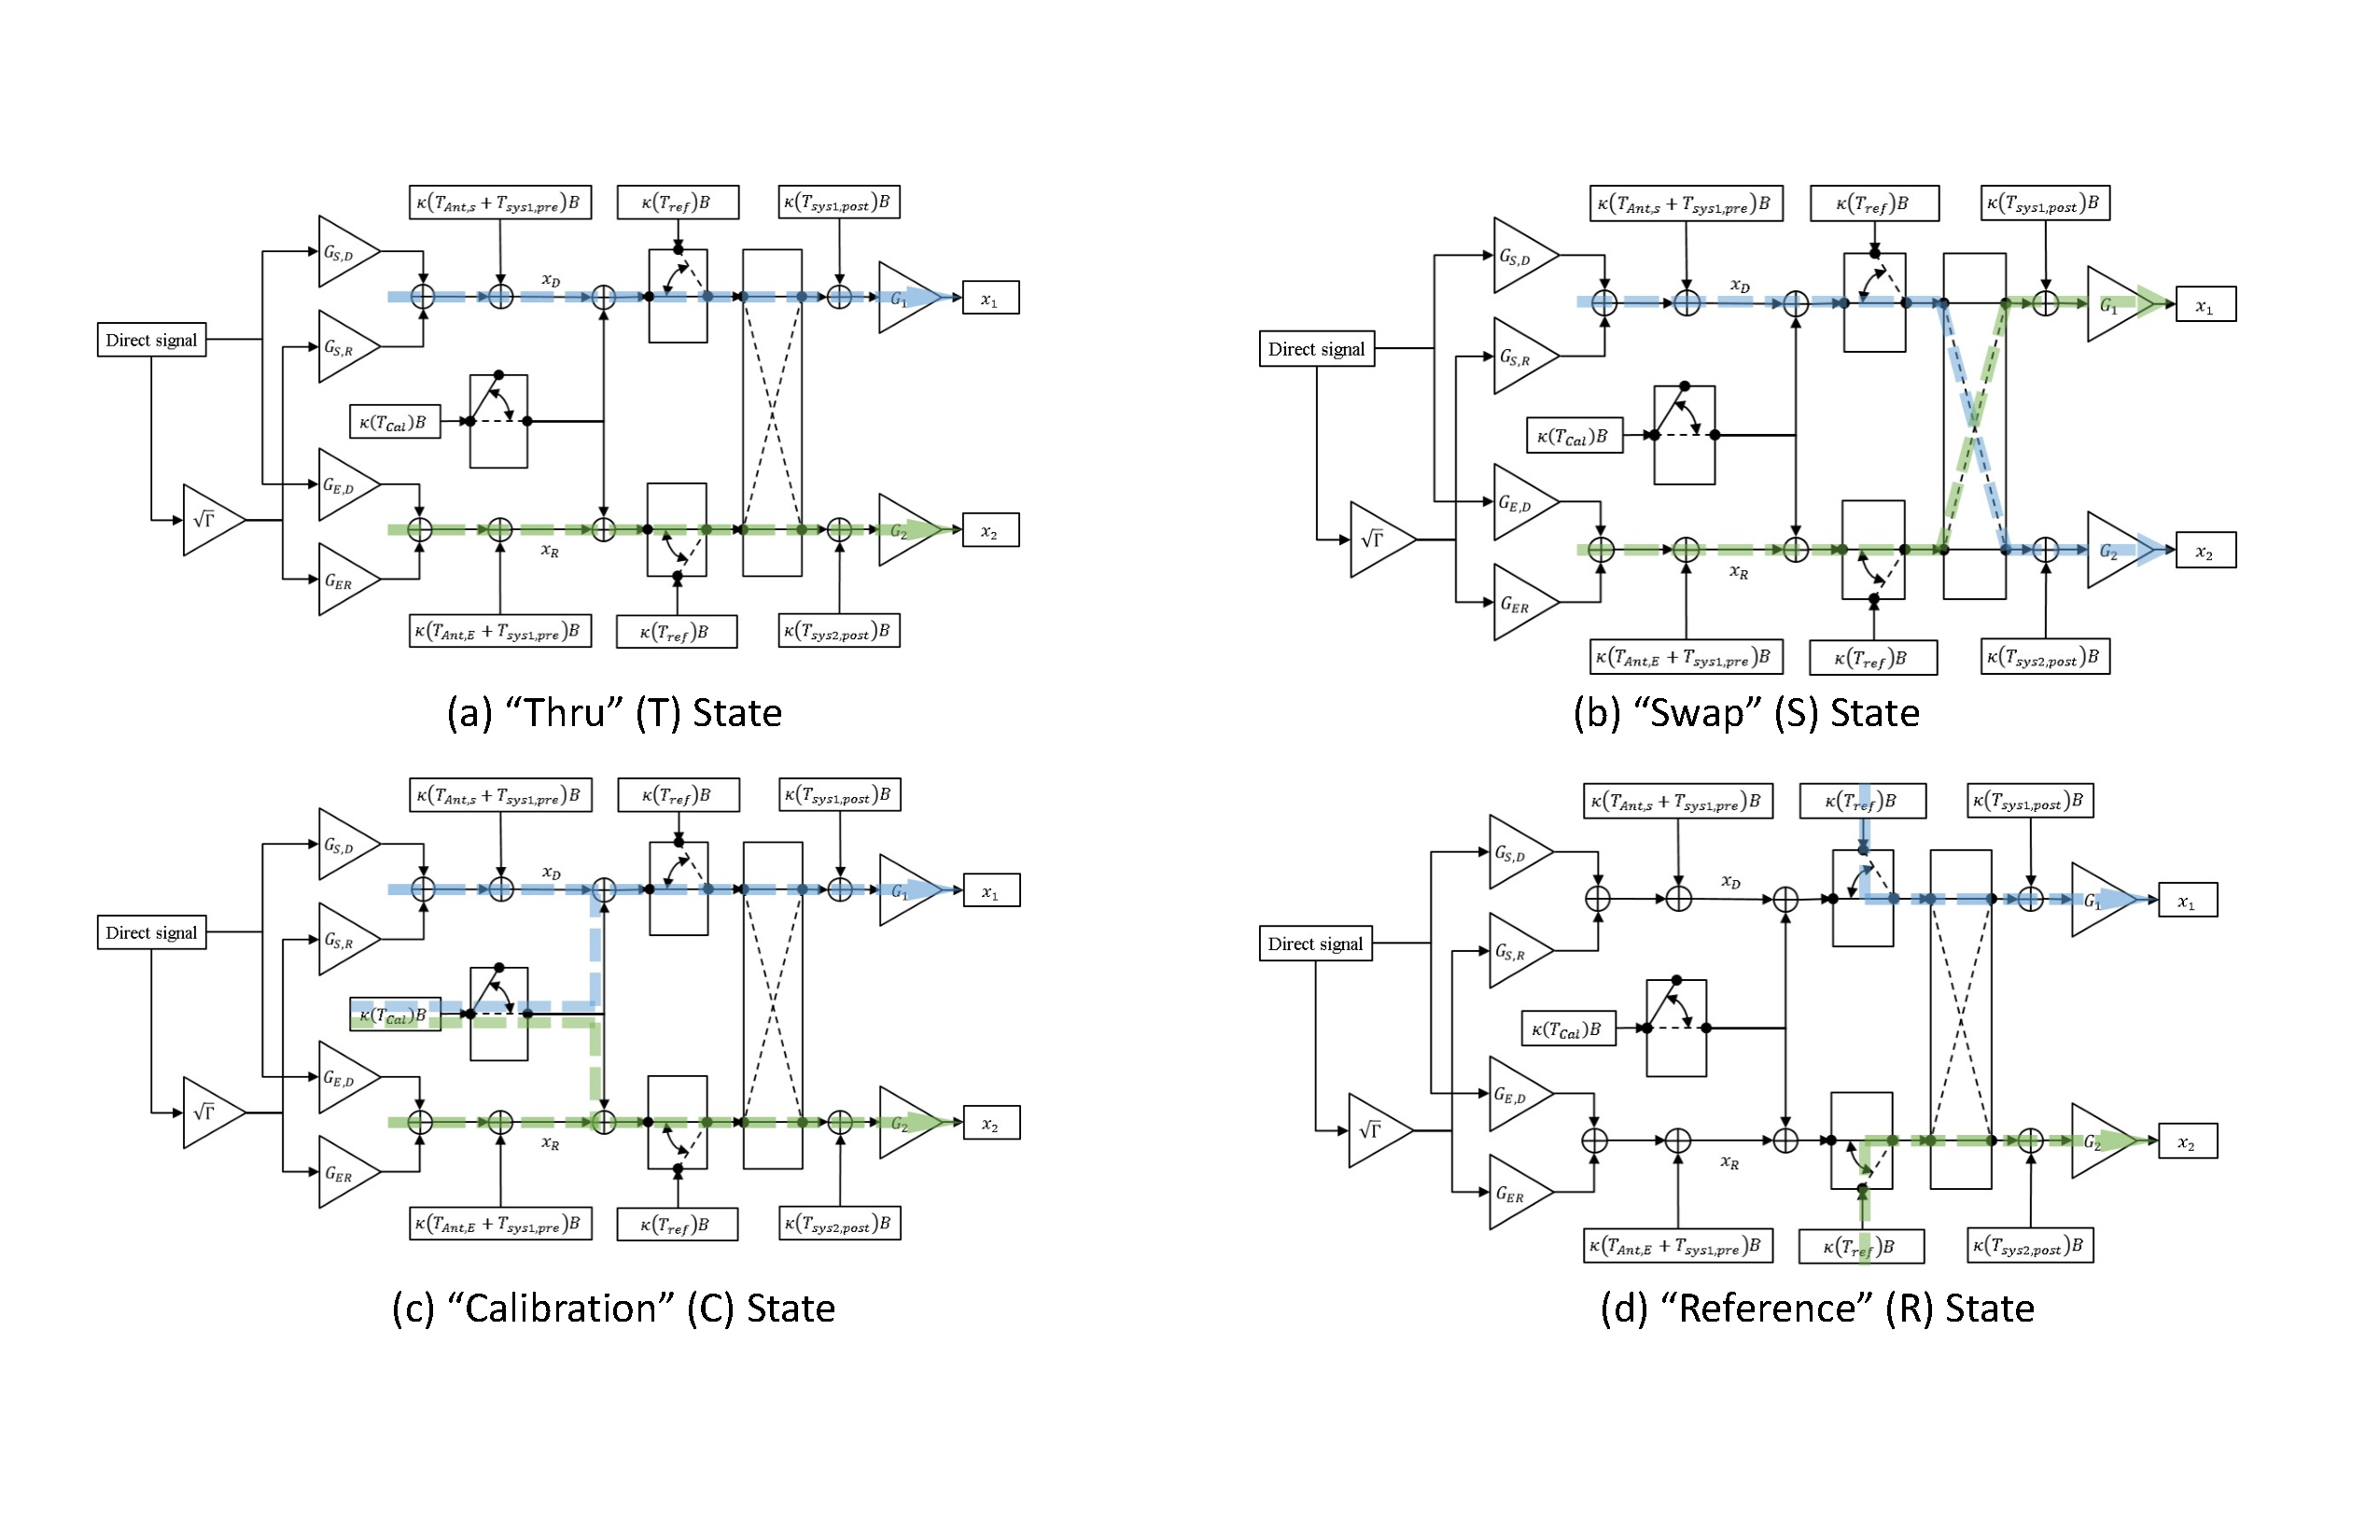
\includegraphics[width=\textwidth]{pdf/receiver_states.pdf}
	\caption{Four states of operation for the receiver. (a) and (b) are the ``thru'' (T) and ``swap'' (S) states, in which the data are collected with a 50\% duty cycle for each state. (c) is the ''Calibration'' (C) state, in which a noise source at temperature $T_{cal}$ is injected into both channels. 
    (d) is the ``Reference'' (R) state, in which the inputs to receivers 1 and 2 are switched to noise sources at temperature $T_{ref}$}
	\centering
	\label{fig:hw_states}
\end{figure}


\subsection{Calibration (C) State}
\label{ssec:cal}
The receiver gains $G_1$ and $G_2$ can be independently estimated through comparing the cross-correlation measurements from the T and C states.
In the C state, a calibrated noise source, at a temperature of $T_{cal}$ is added to both receiver channels 1 and 2. 
Differencing equation (\ref{eqn:observation_eqn_general}) with  $\mathbf{T}_c  = [ \begin{array}{cc} 1 & 1 \end{array}]$ from that with $\mathbf{T}_c  = [ \begin{array}{cc} 0 & 0 \end{array}]$, yields the following 
\begin{equation}
G_m = \frac{Y^C_{m,m}(0) - Y^T_{m,m}(0)}{ k T_{cal} B_N} \,\,\,\,\,\,  m =\left\{1,2\right\}
\label{eqn:calstate}
\end{equation}
%and 
%\begin{equation}
%G_2 = \frac{Y^C_{2,2}(0) - Y^T_{2,2}(0)}{ k T_{cal} B_N} 
%\end{equation}
in which $k$ is the Boltzmann constant. 

%Assuming that all of the parameters remain the same 
%estimated from  $\tilde{R}^n_*$ in Equations \ref{Eq: R11_reduce_norm}-\ref{Eq: R12_reduce_norm} and $\tilde{R}^c_*$ in Equations \ref{Eq: R11_reduce_cal}-\ref{Eq: R12_reduce_cal}, and the noise power from noise load $\sigma^2_{cal}$. The product of channel gain and $\sigma^2_{cal}$ is calculated in
%\begin{eqnarray}
%	\tilde{R}^c_{11}(0) - \tilde{R}^n_{11}(0)&&= G_1\sigma^2_{cal} \label{Eq: Cal_channel_gain1a} \\
  %  \tilde{R}^c_{22}(0) - \tilde{R}^n_{22}(0)&&= G_2\sigma^2_{cal} \label{Eq: Cal_channel_gain2a} \\
  %  \tilde{R}^c_{12}(0) - \tilde{R}^n_{12}(0)&&= \sqrt{G_1 G_2}\sigma^2_{cal} \label{Eq: Cal_channel_gain12a}
%\end{eqnarray}
%Once $\sigma^2_{cal}$ is well measured, 
%\begin{eqnarray}
%	G_1 &&= \frac{\tilde{R}^c_{11}(0) - \tilde{R}^n_{11}(0)}{\sigma^2_{cal}}  \label{Eq: Cal_channel_gain1} \\
  %  G_2 &&= \frac{\tilde{R}^c_{22}(0) - \tilde{R}^n_{22}(0)}{\sigma^2_{cal}}  \label{Eq: Cal_channel_gain2} \\
   % \sqrt{G_1 G_2} &&= \frac{\tilde{R}^c_{12}(0) - \tilde{R}^n_{12}(0)}{\sigma^2_{cal}}  \label{Eq: Cal_channel_gain12}
%\end{eqnarray}



\subsection{Reference (R)  State}
\label{ssec:ref}
%In Figure \ref{fig:Hardware}, $T_{cal}$ is noise temperature of the calibrated noise load, 
In the R-state, the input to the two receivers is switched to  RF terminators having measured noise temperatures of $T_{ref,1}$ and $T_{ref,2}$.
Equation (\ref{Eq:x2_ref_state}) gives the signals at each receiver.  
Computing the cross-correlation matrix, it is straightforward to show that the receiver noise power ($W_1 B_N$ and $W_2 B_N$) can be estimated from the autocorrelations of channel 1 and 2. 
\begin{equation}
W_m B_N = \frac{Y_{m,m}^R(0)}{G_m} - k T_{ref,m} B_N, \,\,\,\,\,\,  m =\left\{1,2\right\}
\label{eqn:refstate}
\end{equation}
%\begin{equation}
%W_2 B_N = \frac{Y_{2,2}^R}{G_2} - k T_{ref,2} B_N
%\end{equation}

\subsection{Antenna Noise Temperature}
\label{ssec:tant}
The total noise power, $N_{1,1}$ or $N_{2,2}$ will be required to form the observable $\Gamma_{o}$. 
%Gains $G_1$, $G_2$ and the receiver noise powers, 
Contributions of the receivers to this noise floor, $W_1 B_N$ and $W_2 B_N$, can be estimated through use of calibration  sources described above. 
The contribution to the noise floor from the antenna noise temperature and the electronics before the transfer switch, $W_S B_N$ and $W_E B_N$, however cannot be estimated from noise injection. 
Models for the sky temperature, incorporating the antenna beam patterns will be used to estimate these contributions.
\bf Manuel ? - more \rm. 

\subsection{Antenna swapping}
Antenna swapping \cite{Alejandro:2013} can also be used for an independent estimate of the ratio of receiver gains %$r_{1,2} = \frac{G_1}{G_2}$ 
which does not involve noise sources. 
$r_{1,2}$ can be found from the ratio of autocorrelation in the T and the S states. 
%and it can be measured by the ratio of $\tilde{R}^s$ Equations \ref{Eq: R11_reduce_swap}-\ref{Eq: R12_reduce_swap} and $\tilde{R}^n$Equations \ref{Eq: R11_reduce_norm}-\ref{Eq: R12_reduce_norm}. When the noise of channels are approximately same, the ratio of channel gain is calculated as
\begin{equation}
  r_{1,2} = \frac{G_1}{G_2} = \frac{Y_{1,1}^S(\tau)}{Y_{2,2}^T(\tau)} = \frac{Y_{1,1}^T(\tau)}{Y_{2,2}^S(\tau)}
  %  \frac{G_1}{G_2} = \frac{\tilde{R}^s_{22}}{\tilde{R}^n_{22}}  
    \label{Eq: Cal_channel_gain_ratio}
\end{equation}

\subsection{Verification Approaches}
We have defined several methods for verifying the calibration results in this section.
The first is to compare the end-to-end retrieval of reflectivity during flights over a flat surface with a know emissivity. 
For example, a lake or inland waterway with a know salinity and temperature. 
%Such flights are already required for the antenna gain pattern calibration, to be described in a forthcoming paper. 

Another type of verification approach is to look for consistency between observables. 
For example, the gain ratio $r_{1,2}$ obtained by antenna swapping in equation (\ref{Eq: Cal_channel_gain_ratio}) must be consistent with the ratio of $G_1$ and $G_2$ produced from the   calibration state in (\ref{eqn:calstate}). 

The following combination of the autocorrelation at lags $0$ and $\tau_{RD}$, produce an  observable independent of that in  
(\ref{Eq:Gamma_estimation_approx}).  
\begin{equation}
\Gamma_o^{'} = \frac{Y_{1,1}^T(\tau_{RD})}{Y_{1,1}^T(0) - N_{1,1}} = f^{'}(\Gamma_a, \phi) + n_{\Gamma}^{'}
\label{eqn:obsverify}
\end{equation}
where 
\begin{equation}
f^{'}(\Gamma, \phi) = \frac{R_a(\tau_{RD}) + \sqrt{I_S \Gamma_a} \left[ e^{j\phi} + R_a(2\tau_{RD}) e^{-j \phi} \right] + \Gamma_a I_S R_a(\tau_{RD}) }
   {1 + 2 \sqrt{I_S \Gamma_a} \mathrm{Re}\left\{ R_a (\tau_{RD}) e^{j \phi}\right\} + \Gamma_a I_s}
\label{eqn:fprime}
\end{equation}

%JLG\section{Measurement Simulation}

To verify the measurement theory, we establish a comprehensive simulator from  satellites to receiver with Matlab. The simulator includes signal resource, path ray of transmitted signal, antenna gain, and receiver parameters.

\subsection{Signal source}
The band

\section{Uncertainty analysis}

Parameters of uncertainty analysis include antenna gains ($G_{S,D}, G_{S,R}, G_{E,D}, G_{E,R}$), channel gain ($G_1, G_2$), noise power spectra ($\sigma_1$), reflectivity ($\Gamma$), and phase ($\phi$).  First, (\ref{eqn:observation_eqn_general}) without noise residual  term is expressed as
\begin{equation}
g(x) = \Gamma_{12}(x) - f(x)
\end{equation}
Where $x=\{G_{S,D}, G_{S,R}, G_{E,D}, G_{E,R}, G_1, G_2, \sigma_1, \Gamma, \phi\}$. $Y_{11}(0)$  and $Y_{12}(\tau^s_{RD})$ are measurement. The full expression of $g(x)$ is
\begin{equation}
g(x) = \sqrt{\frac{G_1}{G_2}} \sqrt{\frac{G_{S,D}}{G_{E,R}}}  
\frac{Y_{12}(\tau^s_{RD})}{Y_{11}(0)-G_1 \sigma^2_1} -
 \frac
{(\sqrt{I_E}+ \sqrt{I_S} \Gamma)R_a(\tau_{RD})+
\sqrt{\Gamma}R_a(0)e^{j\phi}+
\sqrt{I_E I_S\Gamma}R_a(2\tau_{RD})e^{-j \phi } )
}
{(1+I_S \Gamma)R_a(0)+
2 \sqrt{I_S\Gamma}(Re(R_a(\tau_{RD})) )cos\phi
} =0                 
\label{Eq: uncertainty_g_gamma12_f}
\end{equation}
The total derivative of $g(x,\tilde{x})$ is
\begin{align}
dg(x,\tilde{x})&=\sum_{x_i \in \tilde{x}} \frac{\partial(g)}{\partial(x_i)} dx_i \\
\Rightarrow dg(x,\tilde{x})&=\sum_{x_i \in \tilde{x}} (\frac{\partial(\Gamma_{12})}{\partial(x_i)} dx_i - \frac{\partial(f)}{\partial(x_i)}dx_i)
\label{Eq: uncertainty_dg}
\end{align}
The first term is the total derivative of $\Gamma_{12}$, and the following equations shows the partial derivative of different parameters.
\begin{align}
G_1 &:
\sqrt{\frac{G_2}{G_1}}
\sqrt{\frac{G_{S,D}}{G_{E,R}}}
\frac{R_{1,2}(\tau_{RD}) (R_{1,1}(0) + G_1 \sigma_1^2)}
{2G_2(R_{1,1}(0) - G_1 \sigma_1^2)^2 )} \\
G_2 &:
-\sqrt{\frac{G_2}{G_1}}
\sqrt{\frac{G_{S,D}}{G_{E,R}}}
\frac{R_{1,2}(\tau_{RD})}
{2G_2^2(R_{1,1}(0) - G_1 \sigma_1^2) )} \\
G_{S,D} &:
 \sqrt{\frac{G_1}{G_2}}
 \sqrt{\frac{G_{E,R}}{G_{S,D}}}  
\frac{R_{1,2}(\tau^s_{RD})}{2 G_{E,R} (R_{1,1}(0)-G_1 \sigma^2_1)} \\
G_{E,R} &:
 -\sqrt{\frac{G_1}{G_2}}
 \sqrt{\frac{G_{E,R}}{G_{S,D}}}  
\frac{R_{1,2}(\tau^s_{RD})}{2 G_{E,R}^2 (R_{1,1}(0)-G_1 \sigma^2_1)} \\
\sigma_1 &:
\sqrt{\frac{G_1}{G_2}} \sqrt{\frac{G_{S,D}}{G_{E,R}}}  
\frac{2 G_1 \sigma_1 R_{1,2}(\tau^s_{RD})}{(R_{1,1}(0)-G_1 \sigma^2_1)^2} 
\end{align}
The second term is the total derivative of $f(\Gamma, \phi)$, and the partial derivative equations are expressed as follows,
\begin{align}
G_{S,D} :& -\frac{1}{2 G_{S,D}}
\frac{\Gamma \sqrt{I_S} + \sqrt{\Gamma I_E I_S } R_a(2\tau^s _{RD}) e^{j  \phi}}
{(1+I_S \Gamma)R_a(0)+
2 \sqrt{I_S\Gamma}(Re(R_a(\tau^s_{RD})) )cos\phi} +  \nonumber \\
&\frac{1}{ G_{S,D}}\frac
{(\sqrt{I_E}+ \sqrt{I_S} \Gamma)R_a(\tau^s_{RD})+
\sqrt{\Gamma}R_a(0)e^{j\phi}+
\sqrt{I_E I_S\Gamma}R_a(2\tau^s_{RD})e^{-j \phi } )
(\Gamma I_S R_a(0) + \sqrt{\Gamma I_S} Re(R_a(\tau^s_{RD}) cos\phi)
}
{((1+I_S \Gamma)R_a(0)+
2 \sqrt{I_S\Gamma}(Re(R_a(\tau^s_{RD})) )cos\phi)^2
}     \\ 
G_{S,R} :& \frac{1}{2 G_{S,D} \sqrt{I_S}} 
\frac{\Gamma R_a(\tau^s_{RD}) + \Gamma \sqrt{I_E} R_a(2\tau^s_{RD}) e^{-j \phi} }
{(1+I_S \Gamma)R_a(0)+
2 \sqrt{I_S\Gamma}(Re(R_a(\tau^s_{RD})) )cos\phi} +  \nonumber \\
&\frac{1}{G_{S,D} \sqrt{I_S}}\frac
{(\sqrt{I_E}+ \sqrt{I_S} \Gamma)R_a(\tau^s_{RD})+
\sqrt{\Gamma}R_a(0)e^{j\phi}+
\sqrt{I_E I_S\Gamma}R_a(2\tau^s_{RD})e^{-j \phi } )
(\Gamma \sqrt{I_S} R_a(0) + \sqrt{\Gamma} Re(R_a(\tau^s_{RD}) cos\phi)
}
{((1+I_S \Gamma)R_a(0)+
2 \sqrt{I_S\Gamma}(Re(R_a(\tau^s_{RD})) )cos\phi)^2
}    \\
G_{E,D} :& 
\frac{1}{2 G_{E,R} \sqrt{I_E}}
\frac{R_a(\tau^s_{RD}) + \sqrt{\Gamma I_S} R_a(2 \tau^s_{RD}) e^{-j \phi}}
{(1+I_S \Gamma)R_a(0)+
2 \sqrt{I_S\Gamma}(Re(R_a(\tau^s_{RD})) )cos\phi
}  \\
G_{E,R} :& 
-\frac{1}{2 G_{E,R}}
\frac{ \sqrt{I_E} R_a(\tau^s_{RD}) + \sqrt{\Gamma I_S I_E} R_a(2 \tau^s_{RD}) e^{-j \phi}}
{(1+I_S \Gamma)R_a(0)+
2 \sqrt{I_S\Gamma}(Re(R_a(\tau^s_{RD})) )cos\phi
}  \\
\Gamma :& \frac{1}{2 \sqrt{\Gamma}}
\frac{2 \sqrt{\Gamma I_S }R_a(\tau^s_{RD}) + R_a(0) e^{j\phi} +\sqrt{ I_E I_S } R_a(2\tau^s _{RD}) e^{j  \phi}}
{(1+I_S \Gamma)R_a(0)+
2 \sqrt{I_S\Gamma}(Re(R_a(\tau^s_{RD})) )cos\phi} -  \nonumber \\
& \frac{1}{ \sqrt{\Gamma}}
\frac
{(\sqrt{I_E}+ \sqrt{I_S} \Gamma)R_a(\tau^s_{RD})+
\sqrt{\Gamma}R_a(0)e^{j\phi}+
\sqrt{I_E I_S\Gamma}R_a(2\tau^s_{RD})e^{-j \phi } )
(\sqrt{\Gamma} I_S R_a(0) + \sqrt{ I_S} Re(R_a(\tau^s_{RD}) cos\phi)
}
{((1+I_S \Gamma)R_a(0)+
2 \sqrt{I_S\Gamma}(Re(R_a(\tau^s_{RD})) )cos\phi)^2
}  \\
\phi :& 
-\frac{R_a(2\tau^s_{RD}) e^{-j\phi}\sqrt{\Gamma I_E I_S} j - \sqrt{\Gamma}R_a(0)e^{j\phi}j }
{(1+I_S \Gamma)R_a(0)+
2 \sqrt{I_S\Gamma}(Re(R_a(\tau^s_{RD})) )cos\phi} + \nonumber \\
& \frac{1}{ \sqrt{\Gamma}}
\frac
{(\sqrt{I_E}+ \sqrt{I_S} \Gamma)R_a(\tau^s_{RD})+
\sqrt{\Gamma}R_a(0)e^{j\phi}+
\sqrt{I_E I_S\Gamma}R_a(2\tau^s_{RD})e^{-j \phi } )
(2 \sqrt{I_S\Gamma}(Re(R_a(\tau^s_{RD})) )sin\phi)
}
{((1+I_S \Gamma)R_a(0)+
2 \sqrt{I_S\Gamma}(Re(R_a(\tau^s_{RD})) )cos\phi)^2
} 
\end{align}
The uncertainty analysis is to clarify  the relationship between $\Gamma$ and $\tilde{x}$, and we can rewrite (\ref{Eq: uncertainty_dg}) by Taylor expansion.
\begin{align}
& \frac{\partial \Gamma_{12}}{\partial G_1} G_1 + 
\frac{\partial \Gamma_{12}}{\partial G_2} G_2 +
\frac{\partial \Gamma_{12}}{\partial \sigma_1} \sigma_1 + \nonumber \\
&(\frac{\partial \Gamma_{12}}{\partial G_{S,D}} - \frac{\partial f}{\partial G_{S,D}} ) G_{S,D} + 
(\frac{\partial \Gamma_{12}}{\partial G_{E,R}} - \frac{\partial f}{\partial G_{E,R}} ) G_{E,R} - \nonumber \\
&\frac{\partial f}{\partial G_{E,D}} G_{E,D} - 
\frac{\partial f}{\partial G_{S,R}} G_{S,R} -
\frac{\partial f}{\partial \Gamma} \Gamma = 0
\end{align}
We can rearrange the equation as
\begin{align}
\Gamma= 
&\frac{\partial \Gamma}{\partial f}(\frac{\partial \Gamma_{12}}{\partial G_1} G_1 + 
\frac{\partial \Gamma_{12}}{\partial G_2} G_2 +
\frac{\partial \Gamma_{12}}{\partial \sigma_1} \sigma_1 + \nonumber \\
&(\frac{\partial \Gamma_{12}}{\partial G_{S,D}} - \frac{\partial f}{\partial G_{S,D}} ) G_{S,D} + 
(\frac{\partial \Gamma_{12}}{\partial G_{E,R}} - \frac{\partial f}{\partial G_{E,R}} ) G_{E,R} - \nonumber \\
&\frac{\partial f}{\partial G_{E,D}} G_{E,D} -
\frac{\partial f}{\partial G_{S,R}} G_{S,R})
\end{align}
The standard deviation of $\Gamma$ is approximate to
\begin{align}
\sigma^2_\Gamma \approx 
&(\frac{\partial \Gamma}{\partial f} \frac{\partial \Gamma_{12}}{\partial G_1})^2 \sigma^2_{G_1} + 
(\frac{\partial \Gamma}{\partial f} \frac{\partial \Gamma_{12}}{\partial G_2})^2 \sigma^2_{G_2} +
(\frac{\partial \Gamma}{\partial f} \frac{\partial \Gamma_{12}}{\partial \sigma_1})^2 \sigma_1 + \nonumber \\
&(\frac{\partial \Gamma_{12}}{\partial G_{S,D}} - \frac{\partial f}{\partial G_{S,D}} ) G_{S,D} + 
(\frac{\partial \Gamma_{12}}{\partial G_{E,R}} - \frac{\partial f}{\partial G_{E,R}} ) G_{E,R} - \nonumber \\
&\frac{\partial f}{\partial G_{E,D}} G_{E,D} -
\frac{\partial f}{\partial G_{S,R}} G_{S,R})
\end{align}

   
\section{Sensitivity Analysis and Error Budget}

For our analysis we will assume an EIRP of 26~dBW per channel and a channel bandwidth of 25~kHz \cite{Franke1997}.
Various modulations have been proposed, including BPSK \cite{Wadsworth}, Continuous Phase Modulation (CPM), 8-PSK trellis coded modulation (8PSK-TCM) \cite{Battista1998}. 
A minimum spacing of 50-kHz between adjacent channels is assumed \cite{Wadsworth}.
BPSK will be used in our simluation, agreeing with our analysis of recorded signals.  
The proposed operations plan for a flight campaign using this instrument will invovle  capture of the broadcast signal of interst and computing the ``self-ambiguity function'' \cite{Pettersson2000c} to use as an approximation for the baseband autocorrlation function of transmission.
Knowledge of the specific modualtion design and data structure is not required to apply this method. 

[Zenki]
\label{sec:error}
   \begin{itemize}
     \item Error sources: antenna gain calibration uncertainty, aircraft motion, noise calibration uncertainty, etc.
     \item Show sensitivity to error in each one of these and how it maps to error in the retrieval of reflectivity
     \item special case of aircraft motion and integration time.
     \item Summary table for each error source with an RSS of the error - this will be in the form of a budget - our requirements on each component of the system - to meet our working requirement.
     \item End-to-end "ensemble" simulation, of a large number of cases distributed over a range of soil moistures, noise figures, etc ...
   \end{itemize}
   
\subsection{Sensitivity Analysis}
The performance of reflectivity retrieval highly depends on the offset of calibrated terms $(G_1, G_2, G_{S,D}, G_{S,R}, G_{E,D}, G_{E,R}, \sigma_1)$ in Equation \ref{Eq:Gamma_estimation}. Equation \ref{Eq:Gamma_estimation} is rewritten as
\begin{equation}
f(\Gamma, \phi, G_1, G_2, G_{S,D}, G_{S,R}, G_{E,D}, G_{E,R}, \sigma_1) =
	\frac{(\sqrt{I_E}+\sqrt{I_S}\Gamma)R_a(\tau_{RD})+\sqrt{\Gamma} 
    e^{j\phi}+\sqrt{I_S I_E\Gamma} R_a(2\tau_{RD})e^{-j\phi}} 
    {1 + I_S \Gamma + 2 \sqrt{I_S \Gamma} \mathcal{Re}[ R_a(\tau_{RD})] \cos \phi}
        \label{Eq:Gamma_uncertainty}
\end{equation}

To analyze the effect of the calibrated terms,  
From Section \ref{sec: Observable and Forward Model},  includes  . . $\Gamma_{12}$ is an implicit function, and the relationship between $\Gamma$ and the calibrated terms is derived by

\begin{eqnarray}
d\Gamma_{12} = \frac{\partial \Gamma_{12}}{\partial G_1} dG_1 
\end{eqnarray}

\section{Coherent Integration Time Limitations}

\subsection{Aircraft Altitude Variation}

show that the variation cant be more that XXX fraction of a cycle within TI, otherwise the signal does not add coherently

\subsection{Error Due to Finite Integration}

Show that the low "chipping" rate of these communication satellites will give an error in the autocorrlation when computed over a finite time.
In this case, for 25 KHz, a 1 ms integration will only cover 25 bits.  There will be a random error in the use of an approximation derived for infinite signal. 

\section{Simulator}
\section{Measurement Simulation}

To verify the measurement theory, we establish a comprehensive simulator from  satellites to receiver with Matlab. The simulator includes signal resource, path ray of transmitted signal, antenna gain, and receiver parameters.

\subsection{Signal source}
The band
[Zenki]
End 2 end simulator - verify error model.  Start with reflectivity - baseband singal - model of receiver - retrieval - estiamted reflectivity.  Numerical error analysis. 

\section{Summary}

Design of a system presented.  

Antenna gain uncertainty is the largest contribution to the error budget. 

Recently, another P-band allocation (360-380~MHz) is beginning to be utilized for communications. 
The transmission consists of four (4) Spectrally Adaptive Wideband Code Division Multiple Access (SA-WCDCMA) channels
with chipping rates of 3.84~Mchip/s \cite{Zunich2009}.
If it is possible to process the entire 20~MHz spectrum as a single ``noise like'' source, then the range resolution will be reduced to approximately 15~m, eliminating many of the problems in isolating the direct and reflected ray paths. 

\section{Conclusion}
The conclusion goes here.





% if have a single appendix:
%\appendix[Proof of the Zonklar Equations]
% or
%\appendix  % for no appendix heading
% do not use \section anymore after \appendix, only \section*
% is possibly needed

% use appendices with more than one appendix
% then use \section to start each appendix
% you must declare a \section before using any
% \subsection or using \label (\appendices by itself
% starts a section numbered zero.



\appendices

\section{P-band Signal Sources}
[Zenki]
\label{app:signal_source}
   \begin{itemize}
     \item General description of allocation of 230-270 MHz band for Govt use
     \item Published information about UFO - signal design, link budget, and orbits - be sure to cite the source of data
     \item Description of field experiment to verify the properties, including the ambiguity function, nominal values for signal power, persistence of signals, etc ... 
     \item summary of properties of UFO, and reference to table \ref{tab:sysparam}
\item Link budget

To generate the synthetic signal, the EIRP of transmitted signal is analyzed by link budget analysis. The link budget is verified by a field experiment, and the equipment of field experiment includes two amateur Yagi antennas, preamplifier, and USRP software radio receiver. The system noise figure is calculated as a cascaded system in Figure \ref{fig:link_budget}.
\begin{figure}[h]
	\centering
	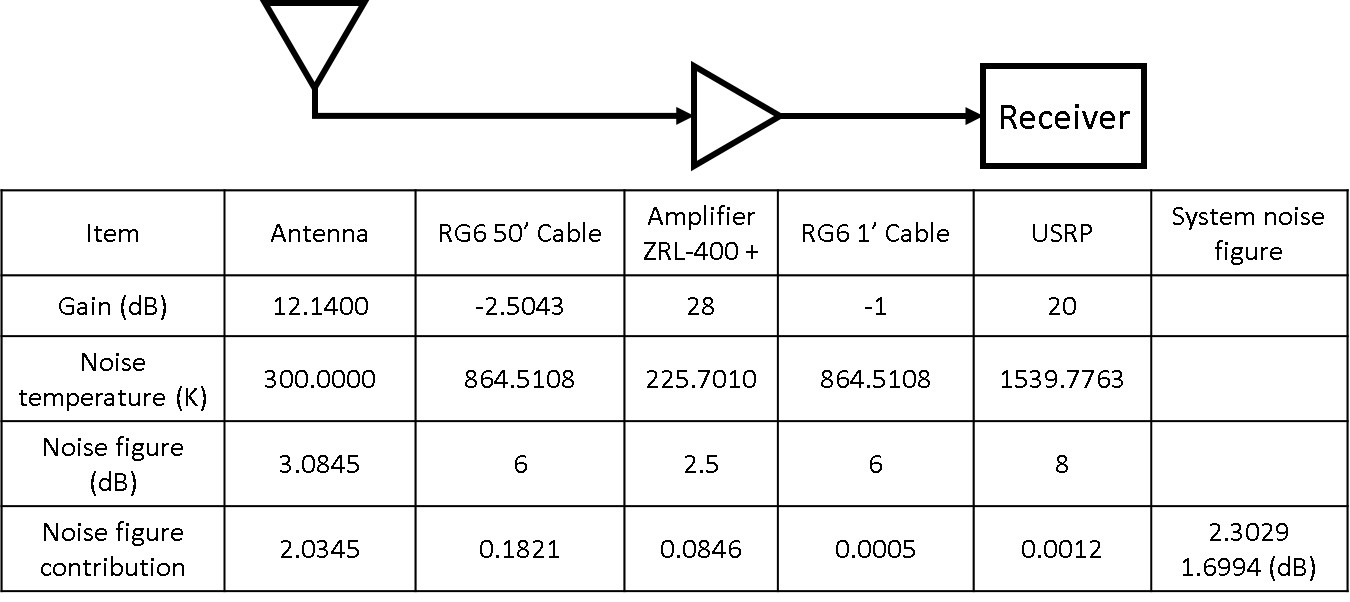
\includegraphics[width=\textwidth]{pdf/Link_budget.jpg}
	\caption{System noise figure includes antenna, cables, amplifier, and receiver.}
	\centering
	\label{fig:link_budget}
\end{figure}
Table \ref{table: link_budget} lists the items of link budget.
\begin{table}[ht]
\centering
\caption{Link budget}
\begin{tabular}{lrl}
\hline
Frequency                        & 260.375    & MHz \\ \hline
Bandwidth                        & 25         & kHz \\ \hline
EIRP                             & 26         & dBW \\ \hline
Fading loss                      & 6          & dB  \\ \hline
Elevation angle                  & 40         & deg \\ \hline
Distance                         & 37780.2664 & km  \\ \hline
Space loss along direct path     & 162.5374   & dB  \\ \hline
Effective area isotropic antenna & 9.7677     & dB  \\ \hline
Received power                   & -152.3051  & dBW \\ \hline
Noise power                      & -159.9958  & dBW \\ \hline
SNR input                        & 7.6907     & dB  \\ \hline
System noise figure              & 1.6994     & dB  \\ \hline
SNR output                       & 5.9913     & dB  \\ \hline
\end{tabular}
\label{table: link_budget}
\end{table}
The observable signal-to-noise ration (SNR) is calculated from the spectrum of the signals collected in the field experiment, and the power of spectrum at 260.35 MHz is set to the noise floor.
\begin{figure}[h]
	\centering
	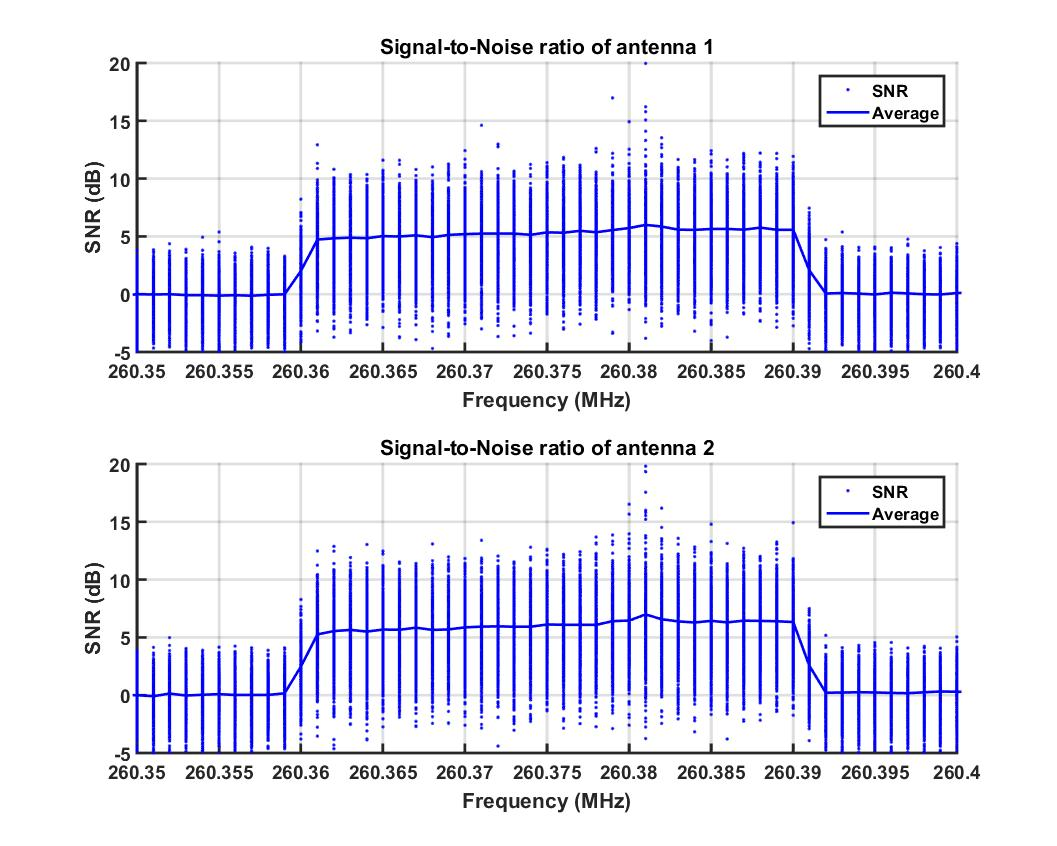
\includegraphics[width=\textwidth]{pdf/SNR.jpg}
	\caption{System noise figure includes antenna, cables, amplifier, and receiver.}
	\centering
	\label{fig:link_budget}
\end{figure}

\item ambigiuty function experimentlaly verified
\item direction finding to validate ephemeris ???
   \end{itemize}
   
   \bf this is directly from Zenki's draft: \rm 
   
   The Ultra High Frequency Follow-On (UFO) system is a communication satellite system whose function is to provide communications for airborne, ship, submarine and ground forces. UFO satellite system is a DOD sponsored program and operated by U.S. Navy. By now there are totally 11 satellites. The first launch is in Mar.1993 and the planned lifetime of UFO system is 14 years. It replaced FLTSATCOM and is scheduled to be replaced by MUOS. The orbit of UFO is geosynchronous orbit and the altitude is 32810 km. From F-1 to F-7, UFO satellites provide redundant command and ranging capabilities when the satellite is on station. The bandwidth of each satellite is 25 kHz and it is on board processing. According to the amateur radio website \cite{Matt:2014}, the frequencies from both satellites are as the following table. Table\ref{Table Band Plan} indicates the location for band plan for UFO satellites.

\begin{table}[ht]
\centering
\begin{tabular}  {|c|c|c|c|c|}
	\hline
     \textbf{Band Plan} & \textbf{November}	& \textbf{Quebec} &	\textbf{Papa} & \textbf{Oscar} \\
    \hline
    Name & UFO F5 & UFO F6 & UFO F7 & UFO F2 \\
    \hline
     Location &	105.6° W & 99.2° W & 	22.0° W	&  28.7° E\\
    \hline
    Name & UFO F11 & UFO F10 & UFO F9  & UFO F3 \\
    \hline
    Location& 71.1° E &	72.6° E &	135.0° E &	156.4° W \\
    \hline
\end{tabular}
\caption{The location and band plan of UFO satellites}
\label{Table Band Plan}
\end{table}

\section{Correlation of modulation of signal} \label{App: Ra}
The modulation of signal is Assumed to be QPSK
\begin{equation}
a(t)=\sum_{q=0}^{\infty}rect(\frac{t-(q+1/2)T_c}{T_c})e^{j(2p(q)+1)\frac{\pi}{4}}
\end{equation}
[JLG - not sure this is needed - isnt this just standard comm theory ? ]

Autocorrelation of a discrete time signal $x[n]$ with finite samples $Nn_c$ is obtained directly by circular convolution or operating from the frequency domain in the following equations.
\begin{equation}\label{Eq: Auto_corx}
\begin{split}
R_x[n] &= \sum\limits_{m=0}^{Nn_c-1} x^*[m] x[n+m \mod Nn_c] \\
	 &= \frac{1}{Nn_c}\sum\limits_{k=0}^{Nn_c-1} X^*[k]X[k] e^{2\pi j \frac{kn}{Nn_c}},
\end{split}
\end{equation}
where $X[k]$ is $x[n]$ in frequency domain by Discrete Fourier Transform (DFT), and the relationship between $x[n]$ and $X[k]$ is expressed in the following equations.
\begin{equation}\label{Eq: xn_XK}
\begin{split}
X[k] &= \sum\limits_{m=0}^{Nn_c-1} x[n] e^{-2\pi j \frac{kn}{Nn_c}} \\
x[n] &= \frac{1}{Nn_c} \sum\limits_{k=0}^{Nn_c-1} X[k] e^{2\pi j \frac{kn}{Nn_c}} 
\end{split}
\end{equation}
Let $a[n]$ denote the discrete time QPSK signal with $Nn_c$ samples and be expressed in the form
\begin{equation}\label{Eq: a_n}
\begin{split}
a[n] &= \sum\limits_{q=0}^{N-1} rect(\frac{nT_s-(q+1/2)T_c}{T_c})e^{j(2\mathcal{U}_q+1)\frac{\pi}{4}} \\ 
	 &= \sum\limits_{q=0}^{N-1} rect(\frac{n-(q+1/2)n_c}{n_c})e^{j(2\mathcal{U}_q+1)\frac{\pi}{4}},    
     \end{split}
\end{equation}
\begin{figure}[t!]
	\centering
	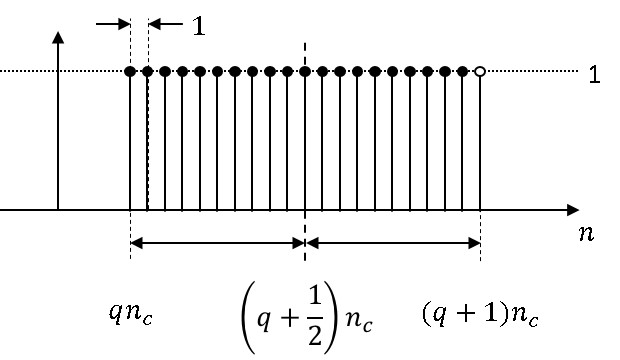
\includegraphics[width=3 in]{pdf/a_n.jpg}
	\caption{The discrete time rectangular function}
	\label{fig:a_n}
\end{figure}
where $T_s$ is the sampling time, $T_c=1/bw$ is the time corresponding to bandwidth ($bw$), $n_c=T_c/T_s$ is the number samples within $T_c$, $N$ represents numbers of $n_c$ ,and $rect$ denotes a rectangular function as shown in Figure \ref{fig:a_n}. $\mathcal{U}_q$ is uniform distribution with integers 0, 1, 2, and 3. To elaborate the autocorrelation of $a[n]$, the autocorrelation of the single rectangular function $c[n]$ is derived first. 
\begin{equation}\label{Eq: c_n}
c[n] = rect(\frac{n-\frac{1}{2} n_c}{n_c})
\end{equation}
The autocorrelation of $c[n]$ is denoted by $d[n]$, and is derived by substituting Equation \ref{Eq: c_n} into Equation \ref{Eq: Auto_corx}
\begin{equation}\label{Eq: d_n}
\begin{split}
d[n] &= \sum\limits_{m=0}^{Nn_c-1} c^*[m] c[n+m] \\
	 &= \sum\limits_{m=0}^{Nn_c-1} rect(\frac{m-\frac{1}{2} n_c}{n_c}) rect(\frac{n+m-\frac{1}{2} n_c \mod Nn_c}{n_c}) \\
     &= \sum\limits_{m=0}^{n_c-1} (n_c-n)\delta[n-m] + 
        \sum\limits_{m=(N-1)n_c-1}^{Nn_c-1} (n-(N-1)n_c-2)\delta[n-m] 
\end{split}
\end{equation}
Figure \ref{fig:c_n_d_n} illustrates $c[n]$ and $d[n]$. The autocorrelation of $c[n]$ in frequency domain is also obtained by Equation \ref{Eq: Auto_corx}.
\begin{equation}\label{Eq: D_k}
\begin{split}
D[k] &= C^*[k] C[k] \\
	 &= (\sum\limits_{n=0}^{Nn_c-1} rect(\frac{n-\frac{1}{2} n_c}{n_c}) e^{-2\pi j \frac{kn}{Nn_c}})^* 
     (\sum\limits_{n=0}^{Nn_c-1} rect(\frac{n-\frac{1}{2} n_c}{n_c}) e^{-2\pi j \frac{kn}{Nn_c}} ) \\
     &= (\frac{ sin(\frac{\pi k}{N})}{sin(\frac{\pi k}{N n_c}}))^2
\end{split}
\end{equation}
\begin{figure}[t!]
	\centering
	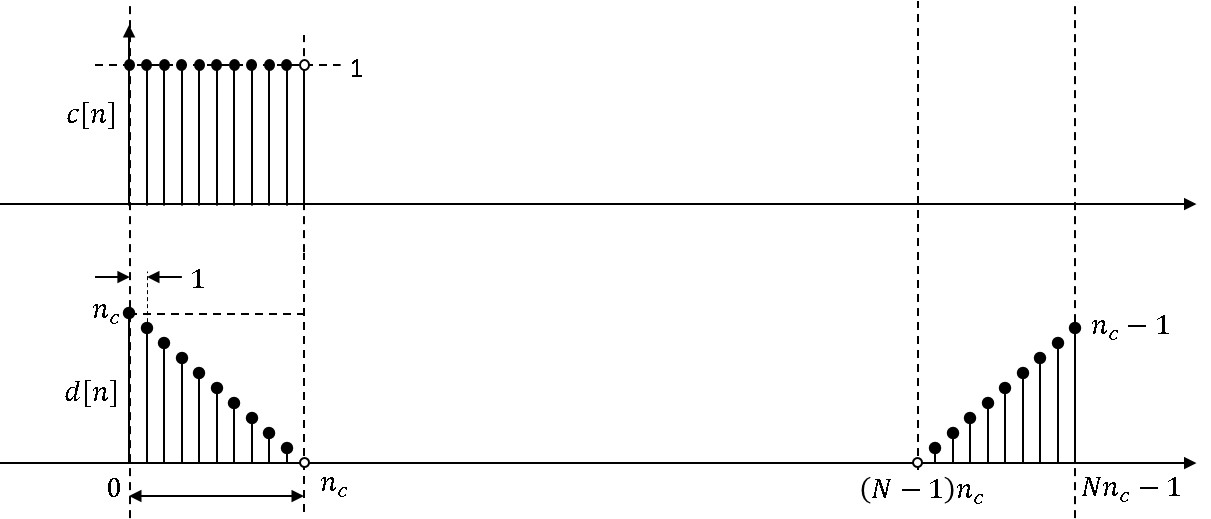
\includegraphics[width=3 in]{pdf/rect_auto.jpg}
	\caption{The discrete time rectangular function}
	\label{fig:c_n_d_n}
\end{figure}
The autocorrelation of $a[n]$ denoted as $R_a[n]$ is derived in 
\begin{equation}\label{Eq: Ra_n}
R_a[n] = \frac{1}{Nn_c}\sum\limits_{k=0}^{Nn_c-1} A^*[k]A[k] e^{2\pi j \frac{kn}{Nn_c}}
\end{equation}
By DFT, $A[k]$ converted from $a[n]$ is given by
\begin{equation}\label{Eq: DFT_a_n}
A[k] = \sum\limits_{n=0}^{Nn_c} a[n]e^{-j2\pi \frac{kn}{Nn_c}}
\end{equation}
After substituting Equation \ref{Eq: a_n} into Equation \ref{Eq: DFT_a_n}, $A[k]$ is derived as
\begin{equation}\label{Eq: A_k}
\begin{split}
A[k] &= \sum\limits_{n=0}^{Nn_c} \sum\limits_{q=0}^{N-1} rect(\frac{n-(q+1/2)n_c}{n_c}) e^{j(2\mathcal{U}_q+1)\frac{\pi}{4}} e^{-j2\pi \frac{kn}{Nn_c}} \\ 
     &= \sum\limits_{q=0}^{N-1} \sum\limits_{n=0}^{Nn_c} rect(\frac{n-(q+1/2)n_c}{n_c}) e^{-j2\pi \frac{kn}{Nn_c}} e^{j(2\mathcal{U}_q+1)\frac{\pi}{4}} \\ 
     &= \sum\limits_{q=0}^{N-1} \sum\limits_{n=qn_c}^{(q+1)n_c} e^{-j2\pi \frac{kn}{Nn_c}} e^{j(2\mathcal{U}_q+1)\frac{\pi}{4}} \\
     &= \frac{1-e^{-j2\pi\frac{k}{N}}} {1-e^{-j2\pi\frac{k}{Nn_c}}} e^{-j2\pi \frac{qk}{N}} \sum\limits_{q=0}^{N-1} e^{j(2\mathcal{U}_q+1)\frac{\pi}{4}} \\
     &= \frac{sin(\pi\frac{k}{N})} {sin(\pi\frac{k}{Nn_c)}} e^{-j\pi \frac{k(n_c-1)}{Nn_c}} \sum\limits_{q=0}^{N-1} e^{-j2\pi \frac{qk}{N}} e^{j(2\mathcal{U}_q+1)\frac{\pi}{4}} 
\end{split}
\end{equation} 
$R_a[n]$ is further derived by substituting Equation \ref{Eq: A_k} into Equation \ref{Eq: Ra_n}.
\begin{equation}\label{Eq: IDFT_Ra1}
\begin{split}
R_a[n] &= \frac{1}{Nn_c}\sum\limits_{k=0}^{Nn_c} D[k] 
\sum\limits_{q=0}^{N-1} \sum\limits_{p=0}^{N-1} 
e^{j(\mathcal{U}_q-\mathcal{U}_p)\frac{\pi}{2}} 
e^{-j2\pi \frac{(q-p)k}{Nn_c}}
e^{j2\pi \frac{kn}{Nn_c}} \\
 &= \sum\limits_{q=0}^{N-1} \sum\limits_{p=0}^{N-1} 
e^{j(\mathcal{U}_q-\mathcal{U}_p)\frac{\pi}{2}} 
\frac{1}{Nn_c}\sum\limits_{k=0}^{Nn_c} D[k] e^{jc\pi \frac{(n-(q-p)n_c) k}{Nn_c}}
\end{split}
\end{equation}
According to Equation \ref{Eq: xn_XK}, $d[n]$ is converted from $D[k]$ by IDFT. After replacing $n$ to $n-(q-p)$, 
\begin{equation}\label{Eq: dn_tmp}
d[n-(q-p)n_c] = \frac{1}{Nn_c} \sum\limits_{k=0}^{Nn_c} D[k] e^{jc\pi \frac{(n-(q-p)n_c) k}{Nn_c}} 
\end{equation}
In the end, the autocorrelation of $a_n$ is simplified as in
\begin{equation}\label{Eq: IDFT_Ra2}
R_a[n] = \sum\limits_{q=0}^{N-1} \sum\limits_{p=0}^{N-1} 
e^{j(\mathcal{U}_q-\mathcal{U}_p)\frac{\pi}{2}} d[n-(q-p)n_c]
\end{equation}
When $q = p$, Equation \ref{Eq: IDFT_Ra2} becomes
\begin{equation}\label{Eq: IDFT_Ra_q_eq_p}
R_a[n] = N d[n]
\end{equation}
If $q \neq p$, The uniform difference distribution $\mathcal{D} = \mathcal{U}_q-\mathcal{U}_p$ of two uniform integers 0, 1, 2, and 3 is found as 
\begin{equation}\label{Eq: diff_uni}
P_{\mathcal{D}}[n] = \frac{4-|n|}{16}, n \in \{ -3,-2,-1,0,1,2,3 \} 
\end{equation}
Equation \ref{Eq: IDFT_Ra2} is rewritten as in
\begin{equation}\label{Eq: IDFT_Ra3}
R_a[n] = \sum\limits_{\substack{q=-(N-1) \\ q\neq 0}}^{N-1} e^{j(\mathcal{D}_q)\frac{\pi}{2}} d[n-q n_c]
\end{equation}
When $p \neq q $, the expected value of $R_a[n]$ is derived in the following equations
\begin{equation}\label{Eq: E_Ra}
\begin{split}
E[R_a[n]] &= \sum\limits_{p=-3}^{p=3} \sum\limits_{\substack{q=-(N-1) \\ q\neq 0}}^{N-1}  e^{j p\frac{\pi}{2}} d[n-q n_c] P_{\mathcal{D}}[p] \\
          &= \sum\limits_{\substack{q=-(N-1) \\ q\neq 0}}^{N-1} d[n-q n_c]  \sum\limits_{p=-3}^{p=3} e^{j p\frac{\pi}{2}}  P_{\mathcal{D}}[p] \\
          &= \sum\limits_{\substack{q=-(N-1) \\ q\neq 0}}^{N-1} d[n-q n_c] [(j) \frac{1}{16} + (-1) \frac{1}{8} + (-j) \frac{3}{16} + (1) \frac{1}{4} + (j) \frac{1}{16} + (1) \frac{1}{16} + (-j) \frac{1}{16}] \\
          &= 0
\end{split}
\end{equation}
By combining Equations \ref{Eq: IDFT_Ra_q_eq_p} and \ref{Eq: E_Ra}, the expected value of $R_a[n]$ is
\begin{equation}\label{Eq: E_Ra2}
E[R_a[n]] = N d[n]
\end{equation}
After subtituing Equation \ref{Eq: d_n} into Equation \ref{Eq: E_Ra2}, the expected value of $R_a[n]$ becomes
\begin{equation}\label{Eq: E_Ra3}
E[R_a[n]] = \sum\limits_{m=0}^{n_c-1} N(n_c-n)\delta[n-m] + 
            \sum\limits_{m=(N-1)n_c-1}^{Nn_c-1} N(n-(N-1)n_c-2)\delta[n-m] 
\end{equation}




\section{Working area- stuff cut out}

Most of this wont be needed - we will replace it with a citation to the relevant papers. I left a much reduced version in the first section of the paper. 


\begin{equation}
\Gamma_{pq} = \left| \mathcal{F}_{pq}(\theta) \right|^2 \Xi (z)
\end{equation}

$\Xi(z)$ is the characteristic function of the PDF of surface heights.  This gives (7) if the surface is Gaussian - leads to the common form in (7)
\begin{equation}
\Gamma_{pq} = \left| \mathcal{F}_{pq}(\theta) \right|^2 \exp \left( - h \cos^2 \theta \right)
\end{equation}

%\section{Soil moisture and reflectivity}
Dielectric constant of soil is a function Reflectivity is estimated by the measurement of SoOp, and the soil Dielectric constant is a very import factor for studying the reflectivity. The dielectric constant of media depends on the properties of media, for example, the dielectric constant of water can be calculated by temperature, salinity, and frequency.


Reflectivity $\Gamma$ is the fraction of incident electromagnetic power that is reflected at an interface. The reflectivity can be represented by Fresnel refection coefficients $\mathcal{R}$.

\begin{equation}
\Gamma = |\mathcal{R}|^2=\frac{P_D}{P_R}
\end{equation}

Where $P_D$ and $P_R$ are the power of direct signal and reflection, respectively. $\mathcal{R}_{hh}$ and $\mathcal{R}_{vv}$ are the co-polar refection coefficients of horizontal plane $(h)$ and vertical plane $(v)$, and they can be expressed as

\begin{equation} 
\begin{split}
	{\mathcal{R}_{hh}} = {}& \frac{{{{\tilde \varepsilon }_r}\cos \theta  - \sqrt 				{{{\tilde \varepsilon }_r} - {{\sin }^2}\theta } }}{{{{\tilde \varepsilon}_r}				\cos \theta  + \sqrt {{{\tilde \varepsilon }_r} - {{\sin }^2}\theta }}}
\\
	{\mathcal{R}_{vv}} = {}& \frac{{\cos \theta  - \sqrt {{{\tilde \varepsilon }_r} - {{\sin }^2}\theta } }}{{\cos \theta  + \sqrt {{{\tilde \varepsilon }_r} - {{\sin }^2}\theta }}} 
    \end{split}
     \label{Eq: reflectivity_di}
\end{equation}

Where $\tilde{\varepsilon}_r$ is the complex relative complex dielectric constant  $\theta$ is the incident angle of signal. The circular polarization cab be transformed by the linear polarization. The transition matrix $\mathcal{T}$ is

\begin{equation*}
	\begin{matrix}
	\hat{u}_{r} = \frac{1}{\sqrt{2}}(\hat{u}_h - j\cdot \hat{u}_v) \\
	\hat{u}_{l} = \frac{1}{\sqrt{2}}(\hat{u}_h + j\cdot \hat{u}_v)
	\end{matrix}
	\Rightarrow 
	\begin{bmatrix}
	\hat{u}_{r} \\
	\hat{u}_{l}
	\end{bmatrix}= \frac{1}{\sqrt{2}}	 
	\begin{bmatrix}
	1 & -j \\
	1 & j
	\end{bmatrix}	
	\begin{bmatrix}
	\hat{u}_{h} \\
	\hat{u}_{v}
	\end{bmatrix}
\end{equation*}

\begin{equation}
	\mathcal{T}_{rl \rightarrow hv} =  \frac{1}{\sqrt{2}}	
	\begin{bmatrix}
	1 & -j \\
	1 & j
	\end{bmatrix}
\end{equation}

The coordinate of co-plane and cross plane for linear polarization and  can be transited to circular polarization by
\begin{equation}
 	\begin{bmatrix}
	\hat{u}_{r}\hat{u}_{r} & \hat{u}_{r}\hat{u}_{l} \\
	\hat{u}_{l}\hat{u}_{r} & \hat{u}_{l}\hat{u}_{l}
	\end{bmatrix} = 
	\begin{bmatrix}
	\hat{u}_{r} \\
	\hat{u}_{l} 
	\end{bmatrix}
	\begin{bmatrix}
	\hat{u}_{r} \\
	\hat{u}_{l} 
	\end{bmatrix}^* = 
	\mathcal{T}_{rl \rightarrow hv}
	\begin{bmatrix}
	\hat{u}_{h}\hat{u}_{h} & \hat{u}_{h}\hat{u}_{v} \\
	\hat{u}_{v}\hat{u}_{h} & \hat{u}_{v}\hat{u}_{v}
	\end{bmatrix}
	\mathcal{T}_{rl \rightarrow hv}^*
\end{equation}

Where $\hat{u}$ is the coordinate, the subscripts $h$ and $v$ represent the horizontal and vertical plane, and the subscripts $r$ and $l$ represent the RHCP and LHCP plane. Then the Fresnel reflection coefficients of the circular polarization are

\begin{equation}
	\begin{bmatrix}
	\mathcal{R}_{rr} & \mathcal{R}_{rl} \\
	\mathcal{R}_{lr} & \mathcal{R}_{ll}
	\end{bmatrix} = 
	\frac{1}{2}
	\begin{bmatrix}
	\mathcal{R}_{hh} + \mathcal{R}_{vv} & \mathcal{R}_{hh} - \mathcal{R}_{vv} \\
	\mathcal{R}_{hh} - \mathcal{R}_{vv} & \mathcal{R}_{hh} + \mathcal{R}_{vv}		\end{bmatrix}
\end{equation}


\bf calibration sections ... \rm
is switched noise temperature of RF terminator, $T_{sys1,pre}$ and $T_{sys2,pre}$is noise of channel 1 and 2, respectively, prior the transfer switch, $T_{sys1,post}$ and $T_{sys2,post}$is noise of channel 1 and 2, respectively, after the transfer switch, and $T_{ant,S}$ and $T_{ant,E}$is noise of sky-view and earth-view antenna, respectively.  The power-spectral density is calcualted by $W_*=\kappa T_*$, and $\kappa$ is the boltmen constant. The signals with activated calibration noise are derived from (\ref{Eq: x2_model})
\begin{equation}
      \left[ \begin{array}{c} \tilde{x}^c_1(t) \\ \tilde{x}^c_2(t) \end{array} \right]  =  \sqrt{C_D}e^{j \omega_{IF} t} \mathbf{G}_R \mathbf{T} \mathbf{G}_A
           \left[ \begin{array}{c} a(t-\tau_D) e^{-j \omega_c \tau_D} \\ \sqrt{\Gamma} a(t-\tau_R) e^{-j \omega_c \tau_R} \end{array} \right]  +
           \left[ \begin{array}{c} n_1(t) \\ n_2(t) \end{array} \right]  +
           \left[ \begin{array}{c} 1 \\ 1 \end{array} \right]  n_{cal}(t) 
           \label{Eq: xcal_model}
\end{equation}
Where tthe power-spectral density of thermal noise the power-spectral density of thermal noise in the through state, $n_1$ and $n_2$ , are
\begin{align}
W_1 = W_{Ant,S} +  W_{sys1,pre} +  W_{sys1,post} \\
W_2 = W_{Ant,E} +  W_{sys2,pre} +  W_{sys2,post}
\end{align}
$W_{cal}$ denotes  the power-spectral density of the activated calibration noise.  The correlation in \ref{eqn:xcorrmat} becomes
 \begin{align}
 \left[ \begin{array}{cc}  \tilde{Y}^c_{1,1}(\tau) & \tilde{Y}^c_{1,2}(\tau) \\ \tilde{Y}^c_{2,1}(\tau) & \tilde{Y}^c_{2,2}(\tau)  \end{array} \right] = 
 &C_D \mathbf{G}_R \mathbf{T} \mathbf{G}_A 
 \left[ \begin{array}{cc} R_a(\tau) & \sqrt{\Gamma} R_a(\tau-\tau_{RD})  e^{j \omega_c \tau_{RD} }  \\ 
    \sqrt{\Gamma} R_a(\tau+\tau_{RD}) e^{-j \omega_c \tau_{RD}} & \Gamma R_a(\tau) \end{array} \right]
 %\mathbf{M} 
 \mathbf{G}_A^T \mathbf{T} \mathbf{G}_R^T + \nonumber \\ &\mathbf{N}_1 + \mathbf{N}_2 + \mathbf{N}_{cal}
 %\label{eqn:xcorrmat}
 \end{align}
The first mode is normal mode which means there is no additional noise in the system, and the correlations $\tilde{R}^n$ in Equation \ref{Eq: R11_reduce}, \ref{Eq: R22_reduce}, and \ref{Eq: R11_reduce} can be rewrote as
\begin{eqnarray}
	\tilde{R}_{11}^n(\tau^s) &&= g^2_{1SD} R_a(\tau^s)e^{j\Delta\omega_e\tau_s}+
G_1(\sigma^2_{Ant,S}+\sigma^2_{sys1,pre} +\sigma^2_{sys1,post}) \delta(\tau^s)                                      
\label{Eq: R11_reduce_norm} \\
	\tilde{R}_{22}^n(\tau^s) &&= g^2_{2ER} R_a(\tau^s)e^{j\Delta\omega_e\tau_s}+
G_2(\sigma^2_{Ant,E}+\sigma^2_{sys2,pre} +\sigma^2_{sys2,post}) \delta(\tau^s)                                       
\label{Eq: R22_reduce_norm} \\
	\tilde{R}_{12}^n(\tau^s) &&= g_{1SD} g_{2ER} R_a(\tau^s-\tau^s_{RD})e^{j\omega_e \tau_{RD}} e^{j\Delta\omega_e\tau_s}  
\label{Eq: R12_reduce_norm}
\end{eqnarray}
Once the transfer switch is activated, the the correlations $\tilde{R}^s$ become
\begin{eqnarray}
\tilde{R}_{11}^s(\tau^s) &&= g^2_{1ER} R_a(\tau^s)e^{j\Delta\omega_e\tau_s}+
G_1(\sigma^2_{Ant,E}+\sigma^2_{sys2,pre} +\sigma^2_{sys1,post}) \delta(\tau^s)                                       
\label{Eq: R22_reduce_swap} \\
\tilde{R}_{22}^s(\tau^s) &&= g^2_{2SD} R_a(\tau^s)e^{j\Delta\omega_e\tau_s}+
G_2(\sigma^2_{Ant,S}+\sigma^2_{sys1,pre} +\sigma^2_{sys2,post}) \delta(\tau^s)                                      
\label{Eq: R11_reduce_swap} \\
	\tilde{R}_{12}^s(\tau^s) &&= g_{1SD} g_{2ER} R_a(\tau^s+\tau^s_{RD})e^{-j\omega_e \tau_{RD}} e^{j\Delta\omega_e\tau_s}  
\label{Eq: R12_reduce_swap}
\end{eqnarray}
When the system injects noise from noise load, the the correlations $\tilde{R}^c$ is changed as
\begin{eqnarray}
	\tilde{R}_{11}^c(\tau^s) &&= g^2_{1SD} R_a(\tau^s)e^{j\Delta\omega_e\tau_s}+
G_1(\sigma^2_{Ant,S}+\sigma^2_{sys1,pre} +\sigma^2_{sys1,post}+\sigma^2_{cal}) \delta(\tau^s)                                      
\label{Eq: R11_reduce_cal} \\
	\tilde{R}_{22}^n(\tau^s) &&= g^2_{2ER} R_a(\tau^s)e^{j\Delta\omega_e\tau_s}+
G_2(\sigma^2_{Ant,E}+\sigma^2_{sys2,pre} +\sigma^2_{sys2,post}+\sigma^2_{cal}) \delta(\tau^s)                                       
\label{Eq: R22_reduce_cal} \\
	\tilde{R}_{12}^n(\tau^s) &&= g_{1SD} g_{2ER} R_a(\tau^s-\tau^s_{RD})e^{j\omega_e \tau_{RD}} e^{j\Delta\omega_e\tau_s}\delta(\tau^s)+
    \sqrt{G_1 G_2}\sigma^2_{cal}\delta(\tau^s)  
\label{Eq: R12_reduce_cal}
\end{eqnarray}The last mode switches the signal sources to reference load in the following equation.
\begin{eqnarray}
	\tilde{R}_{11}^r(\tau^s) &&= G_1(\sigma^2_{REF}+\sigma^2_{sys1,post}) \delta(\tau^s)                                      
\label{Eq: R11_reduce_ref} \\
	\tilde{R}_{22}^r(\tau^s) &&= G_2(\sigma^2_{REF}+\sigma^2_{sys2,post}) \delta(\tau^s)                                
\label{Eq: R22_reduce_ref} \\
	\tilde{R}_{12}^r(\tau^s) &&= 0 
\label{Eq: R12_reduce_ref}
\end{eqnarray}

The noise of channel 1 and 2 after the transfer switch are further estimated by substituting $G_1$ and $G_2$ into Equations \ref{Eq: R11_reduce_ref} and \ref{Eq: R22_reduce_ref}. The Equations \ref{Eq: R11_reduce_ref} and \ref{Eq: R22_reduce_ref} are rewrote as
\begin{eqnarray}
	\sigma^2_{sys1,post} &&= \frac{\tilde{R}^r_{11}(0) }{G_1}-\sigma^2_{REF}  \label{Eq: Cal_channel_noise1} \\
    \sigma^2_{sys2,post} &&= \frac{\tilde{R}^r_{22}(0) }{G_2}-\sigma^2_{REF}  \label{Eq: Cal_channel_noise2} 
\end{eqnarray}



% Note that the IEEE does not put floats in the very first column
% - or typically anywhere on the first page for that matter. Also,
% in-text middle ("here") positioning is typically not used, but it
% is allowed and encouraged for Computer Society conferences (but
% not Computer Society journals). Most IEEE journals/conferences use
% top floats exclusively. 
% Note that, LaTeX2e, unlike IEEE journals/conferences, places
% footnotes above bottom floats. This can be corrected via the
% \fnbelowfloat command of the stfloats package.

%\section{Dielectric constant of the soil}
%\label{sec:DC_soil}
Dieletric constant of soil mixture depends on the frequency, temperature, salinity of soil, the bulk soil density, and soil moisture \cite{Peplinski:1995,Peplinski_correct:1995}.

\begin{equation} \label{eq: soil_dielectric_main}
\begin{split}
		 { \varepsilon_{soil} } &=  { \varepsilon'_{soil} } -j { \varepsilon''_{soil} } \\
    	 { \varepsilon'_{soil} } &= [1 + \frac{\rho_b}{\rho_{ss}} ( {\varepsilon_{s}^{\alpha}}-1) + (m_v^{\beta'}\varepsilon_{fw}^{\prime\alpha}-m_v]^{1/\alpha} \\
         { \varepsilon''_{soil} } &=m_v^{\beta"}\varepsilon_{fw}^{''\alpha}
\end{split}
\end{equation}

Where $\varepsilon_{soil}$ is the dielectric constant of soil, $\rho_b$ is the bulk density, $\rho_{ss}$ is the density of the solid soil material, $\varepsilon'_{fw}$ and $\varepsilon''_{fw}$ are the real and imaginary part of the dielectric constant of the free water, and $\alpha=0.65$ and $\beta$ are adjustable parameters. The adjustable parameters $\beta$ is a function of soil texture as follows,

\begin{equation}
\begin{split}
	\beta' &= 1.2748-0.519Soil_{sand}-0.152Soil_{clay} \\
    \beta'' &=1.33797-0.603Soil_{sand}-0.166Soil_{clay}
 \end{split}
\end{equation}
where $S$ and $C$ represent the mass fractions of sand and clay, respectively. The bulk density is also a function of soil texture \cite{Saxton:1986}.

\begin{equation} \label{eq: bulk_density}
\begin{split}
	 \rho_b &= (1-\Psi)\rho_b \\
	  \Psi &= 0.332 - 7.251 \cdot 10^{-4} Soil_{sand} + 0.1276 log_{10}(Soil_{clay})
\end{split}
\end{equation}

$\varepsilon_{s} $ is the dielectric constant of the solid soil is given by
\begin{equation}
	\varepsilon_s = (1.01+0.44\rho_s)^2-0.062
\end{equation}
The dielectric constant of free water $\varepsilon'_{fw}$ and $\varepsilon''_{fw}$ are expressed as the follows,
\begin{equation}
\begin{split}
	\varepsilon'_{fw} &=\varepsilon_{w\infty} + \frac{\varepsilon_{w0}-\varepsilon_{w\infty}}{1+(2 \pi f \tau_w)^2} \\
    \varepsilon''_{fw} &=\frac{2 \pi f \tau_w(\varepsilon_{w0}-\varepsilon_{w\infty})}{1+(2 \pi f \tau_w)^2} + \frac{\sigma_{eff}}{2 \pi \varepsilon_0 f} \frac{\rho_s-\rho_b}{\rho_s m_v} 
\end{split}
\end{equation}
where $\varepsilon_0$ is the permittivity of free space, $\tau_w$ represents the relaxation time for water, $f$ is the frequency in Hz, $\varepsilon_{w\infty}$ = 4.9 is the high-frequency limit of $\varepsilon'_{fw}$, and $m_v$ is the Volumetric soil moisture. The effective conductivity $\sigma_{eff}$ can be estimated as
\begin{equation}
	\sigma_{eff} = 0.0467+0.2204\rho_b-0.4111Soil_{sand}+0.6614Soil_{clay}
\end{equation}


\begin{table}[ht]
\centering
\begin{tabular}  {|c|c|c|c|c|c|}
	\hline
     Polynomial &1&2 &3&4&5\\
    \hline
   P-Band & 372.81 & -1200.41 &	1709.41 & -1390.75 & 710.29\\
     \hline
     Polynomial &6&7&8&9 &10\\
    \hline
   P-Band & -232.89 &	49.53 &	-5.68 & 0.84 & -0.04 \\
    \hline
\end{tabular}
\caption{The coefficients of a polynomial of degree 9}
\label{Table:Polynomial_fitting}
\end{table}


\bf This is just a derivation of Newton's method ... \rm
\begin{eqnarray}
f_{Re}(\Gamma, \phi)=&\frac{(\sqrt{I_E}+\sqrt{I_S}\Gamma)R_a(\tau^s_{RD})+(\sqrt{\Gamma} R_a(0)+\sqrt{I_S I_E\Gamma} R_a(2\tau^s_{RD}))cos\phi}                              
                   {(1 + I_S)\Gamma)R_a(0)+2\sqrt{I_S\Gamma} R_a(\tau^s_{RD})cos\phi}   \\
f_{Im}(\Gamma, \phi)=&\frac{(\sqrt{\Gamma} R_a(0)-\sqrt{I_S I_E\Gamma} R_a(2\tau^s_{RD}))sin\phi }                             
                   {(1 + I_S)\Gamma)R_a(0)+2\sqrt{I_S\Gamma} R_a(\tau^s_{RD})cos\phi}   
    \label{Eq: Gamma_estimation_approx2}
\end{eqnarray}
The jacobian matrix of Equation \ref{Eq: Gamma_estimation_approx2} is as the following matrix, 
\begin{equation}
    J(\Gamma, \phi) =
    \begin{bmatrix}
        \frac{\partial f_{Re}}{\partial \Gamma}      &  \frac{\partial f_{Re}}{\partial \phi}  \\
        \frac{\partial f_{Im}}{\partial \Gamma}      &  \frac{\partial f_{Im}}{\partial \phi}  
    \end{bmatrix} \label{Eq: Jacobian}
\end{equation}

The reflectivity can be estimated from Equation \ref{Eq: Gamma_estimation_approx2} by the iteration. At first, the initial solutions $(\Gamma^{(0)}, \phi^{(0)})$ are substituted into \ref{Eq: Gamma_estimation_approx2}, the difference between the measurement  and estimation is  
\begin{equation}
\begin{bmatrix} \Delta f_{Re}^{(0)} \\ \Delta f_{Im}^{(0)} \end{bmatrix} = 
\begin{bmatrix} f_{Re}(\Gamma, \phi) -  f_{Re}(\hat{\Gamma}^{(0)}, \hat{\phi}^{(0)})\\ f_{Im}(\Gamma, \phi) -  f_{Im}(\hat{\Gamma}^{(0)}, \hat{\phi}^{(0)})\end{bmatrix}
\label{Eq: LSQ1}
\end{equation}
The solutions of reflectivity and phase can be updated as
\begin{align}
 \begin{bmatrix} \Delta \Gamma^{(0)} \\ \Delta \phi^{(0)} \end{bmatrix} &=
 \begin{bmatrix}
        \frac{\partial f_{Re}}{\partial \Gamma}      &  \frac{\partial f_{Re}}{\partial \phi}  \\
        \frac{\partial f_{Im}}{\partial \Gamma}      &  \frac{\partial f_{Im}}{\partial \phi}  
    \end{bmatrix} ^{-1} _{(\hat{\Gamma}^{(0)} ,\hat{\phi}^{(0)})}
    \begin{bmatrix} \Delta f_{Re}^{(0)} \\ \Delta f_{Im}^{(0)} \end{bmatrix} \\
\begin{bmatrix} \hat{\Gamma}^{(1)} \\\hat{\phi}^{(1)} \end{bmatrix}  &= 
\begin{bmatrix} \hat{\Gamma}^{(0)} \\ \hat{\phi}^{(0)} \end{bmatrix}  + \begin{bmatrix} \Delta \Gamma^{(0)} \\ \Delta \phi^{(0)} \end{bmatrix}
\label{Eq: LSQ2}
\end{align}
The final solutions are obtained until  the difference between the measurement  and estimation $(\Delta f_{Re}^{(n)} , \Delta f_{Im}^{(n)}) $  are smaller than tolerance.
\begin{align}
 \begin{bmatrix} \Delta \Gamma^{(n-1)} \\ \Delta \phi^{(n-1)} \end{bmatrix} &=
 \begin{bmatrix}
        \frac{\partial f_{Re}}{\partial \Gamma}      &  \frac{\partial f_{Re}}{\partial \phi}  \\
        \frac{\partial f_{Im}}{\partial \Gamma}      &  \frac{\partial f_{Im}}{\partial \phi}  
    \end{bmatrix} ^{-1} _{(\hat{\Gamma}^{(n-1)} ,\hat{\phi}^{(n-1)})}
    \begin{bmatrix} \Delta f_{Re}^{(n-1)} \\ \Delta f_{Im}^{(n-1)} \end{bmatrix} \\
\begin{bmatrix} \hat{\Gamma}^{(n)} \\ \hat{\phi}^{(n)} \end{bmatrix}  &= 
\begin{bmatrix} \hat{\Gamma}^{(n-1)} \\ \hat{\phi}^{(n-1)} \end{bmatrix}  + \begin{bmatrix} \Delta \Gamma^{(n-1)} \\ \Delta \phi^{(n-1} \end{bmatrix} \\
\begin{bmatrix} \Delta f_{Re}^{(n)} \\ \Delta f_{Im}^{(n)} \end{bmatrix} &= 
\begin{bmatrix} f_{Re}(\Gamma, \phi) -  f_{Re}(\Gamma^{(n-1)}, \phi^{(n-1)})\\ f_{Im}(\Gamma, \phi) -  f_{Im}(\Gamma^{(n-1)}, \phi^{(n-1)})\end{bmatrix}
\label{Eq: LQS3}
\end{align}


% use section* for acknowledgment
\section*{Acknowledgment}


The authors would like to thank...


% Can use something like this to put references on a page
% by themselves when using endfloat and the captionsoff option.
\ifCLASSOPTIONcaptionsoff
  \newpage
\fi



% trigger a \newpage just before the given reference
% number - used to balance the columns on the last page
% adjust value as needed - may need to be readjusted if
% the document is modified later
%\IEEEtriggeratref{8}
% The "triggered" command can be changed if desired:
%\IEEEtriggercmd{\enlargethispage{-5in}}

% references section

% can use a bibliography generated by BibTeX as a .bbl file
% BibTeX documentation can be easily obtained at:
% http://www.ctan.org/tex-archive/biblio/bibtex/contrib/doc/
% The IEEEtran BibTeX style support page is at:
% http://www.michaelshell.org/tex/ieeetran/bibtex/
%\bibliographystyle{IEEEtran}
% argument is your BibTeX string definitions and bibliography database(s)
%\bibliography{IEEEabrv,../bib/paper}
%
% <OR> manually copy in the resultant .bbl file
% set second argument of \begin to the number of references
% (used to reserve space for the reference number labels box)


\bibliography{mendeley}

%
% Use bibtex.
%
%  Zenki's original bibliography
%
%\begin{thebibliography}{1}

%\bibitem{Ulaby:1981}
%F. T. Ulaby, R. K. Moore, and A. K. Fung, Microwave Remote Sensing: From theory to applications: Addison-Wesley Publishing Company, Advanced Book Program/World Science Division, 1981.

%\bibitem{Saxton:1986}
%K. E. Saxton, W. J. Rawls, J. S. Romberger, and R. I. Papendick, "Estimating Generalized Soil-water Characteristics from Texture1," Soil Sci. Soc. Am. J., vol. 50, pp. 1031-1036, 1986 1986.

%\bibitem{Peplinski:1995}
%5N. R. Peplinski, F. T. Ulaby, and M. C. Dobson, "Dielectric properties of soils in the 0.3-1.3-GHz range," Geoscience and Remote Sensing, IEEE Transactions on, vol. 33, pp. 803-807, 1995.

%\bibitem{Peplinski_correct:1995}
%N. R. Peplinski, F. T. Ulaby, and M. C. Dobson, "Corrections to "Dielectric Properties of Soils in the 0.3-1.3-GHz Range"," Geoscience and Remote Sensing, IEEE Transactions on, vol. 33, p. 1340, 1995.

%\bibitem{Jin:2011}
%S. Jin, G. P. Feng, and S. Gleason, "Remote sensing using GNSS signals: Current status and future directions," Advances in Space Research, vol. 47, pp. 1645-1653, 5/17/ 2011.

%\bibitem{Zavorotny:2010}
%V. U. Zavorotny, K. M. Larson, J. J. Braun, E. E. Small, E. D. Gutmann, and A. L. Bilich, "A Physical Model for GPS Multipath Caused by Land Reflections: Toward Bare Soil Moisture Retrievals," Selected Topics in Applied Earth Observations and Remote Sensing, IEEE Journal of, vol. 3, pp. 100-110, 2010.

%\bibitem{Matt:2014}
%K. Rautiainen, J. Lemmetyinen, M. Schwank, A. Kontu, C. B. Ménard, C. Mätzler, et al., "Detection of soil freezing from L-band passive microwave observations," Remote Sensing of Environment, vol. 147, pp. 206-218, 5/5/ 2014.

%\bibitem{Larson:2008}
%K. M. Larson, E. E. Small, E. D. Gutmann, A. L. Bilich, J. J. Braun, and V. U. Zavorotny, "Use of GPS receivers as a soil moisture network for water cycle studies," Geophys. Res. Lett., vol. 35, p. L24405, 2008.

%\bibitem{Shah:2011}
%R. Shah, J. L. Garrison, and M. S. Grant, "Anisotropy in ocean scattering of bistatic radar using signals of opportunity," in Geoscience and Remote Sensing Symposium (IGARSS), 2011 IEEE International, 2011, pp. 4229-4232.

%\bibitem{Kerr:2000}
%Y. H. Kerr, J. Font, P. Waldteufel, and M. Berger, "The Soil Moisture and Ocean Salinity Mission - SMOS," in ESA Earth Observation Quarterly, ed, 2000, pp. 18-25.

%\bibitem{Wang:2009}
%L. Wang and J. J. Qu, "Satellite remote sensing applications for surface soil moisture monitoring: A review," Frontiers of Earth Science in China, vol. 3, pp. 237-247, 2009.

%\bibitem{Entekhabi:2010}
%D. Entekhabi, E. G. Njoku, P. E. O'Neill, K. H. Kellogg, W. T. Crow, W. N. Edelstein, et al., "The Soil Moisture Active Passive (SMAP) Mission," PROCEEDINGS OF THE IEEE, vol. 98, pp. 704-716, 2010.

%\end{thebibliography}

% biography section
% 
% If you have an EPS/PDF photo (graphicx package needed) extra braces are
% needed around the contents of the optional argument to biography to prevent
% the LaTeX parser from getting confused when it sees the complicated
% \includegraphics command within an optional argument. (You could create
% your own custom macro containing the \includegraphics command to make things
% simpler here.)
%\begin{IEEEbiography}[{\includegraphics[width=1in,height=1.25in,clip,keepaspectratio]{mshell}}]{Michael Shell}
% or if you just want to reserve a space for a photo:


\begin{IEEEbiography}
[{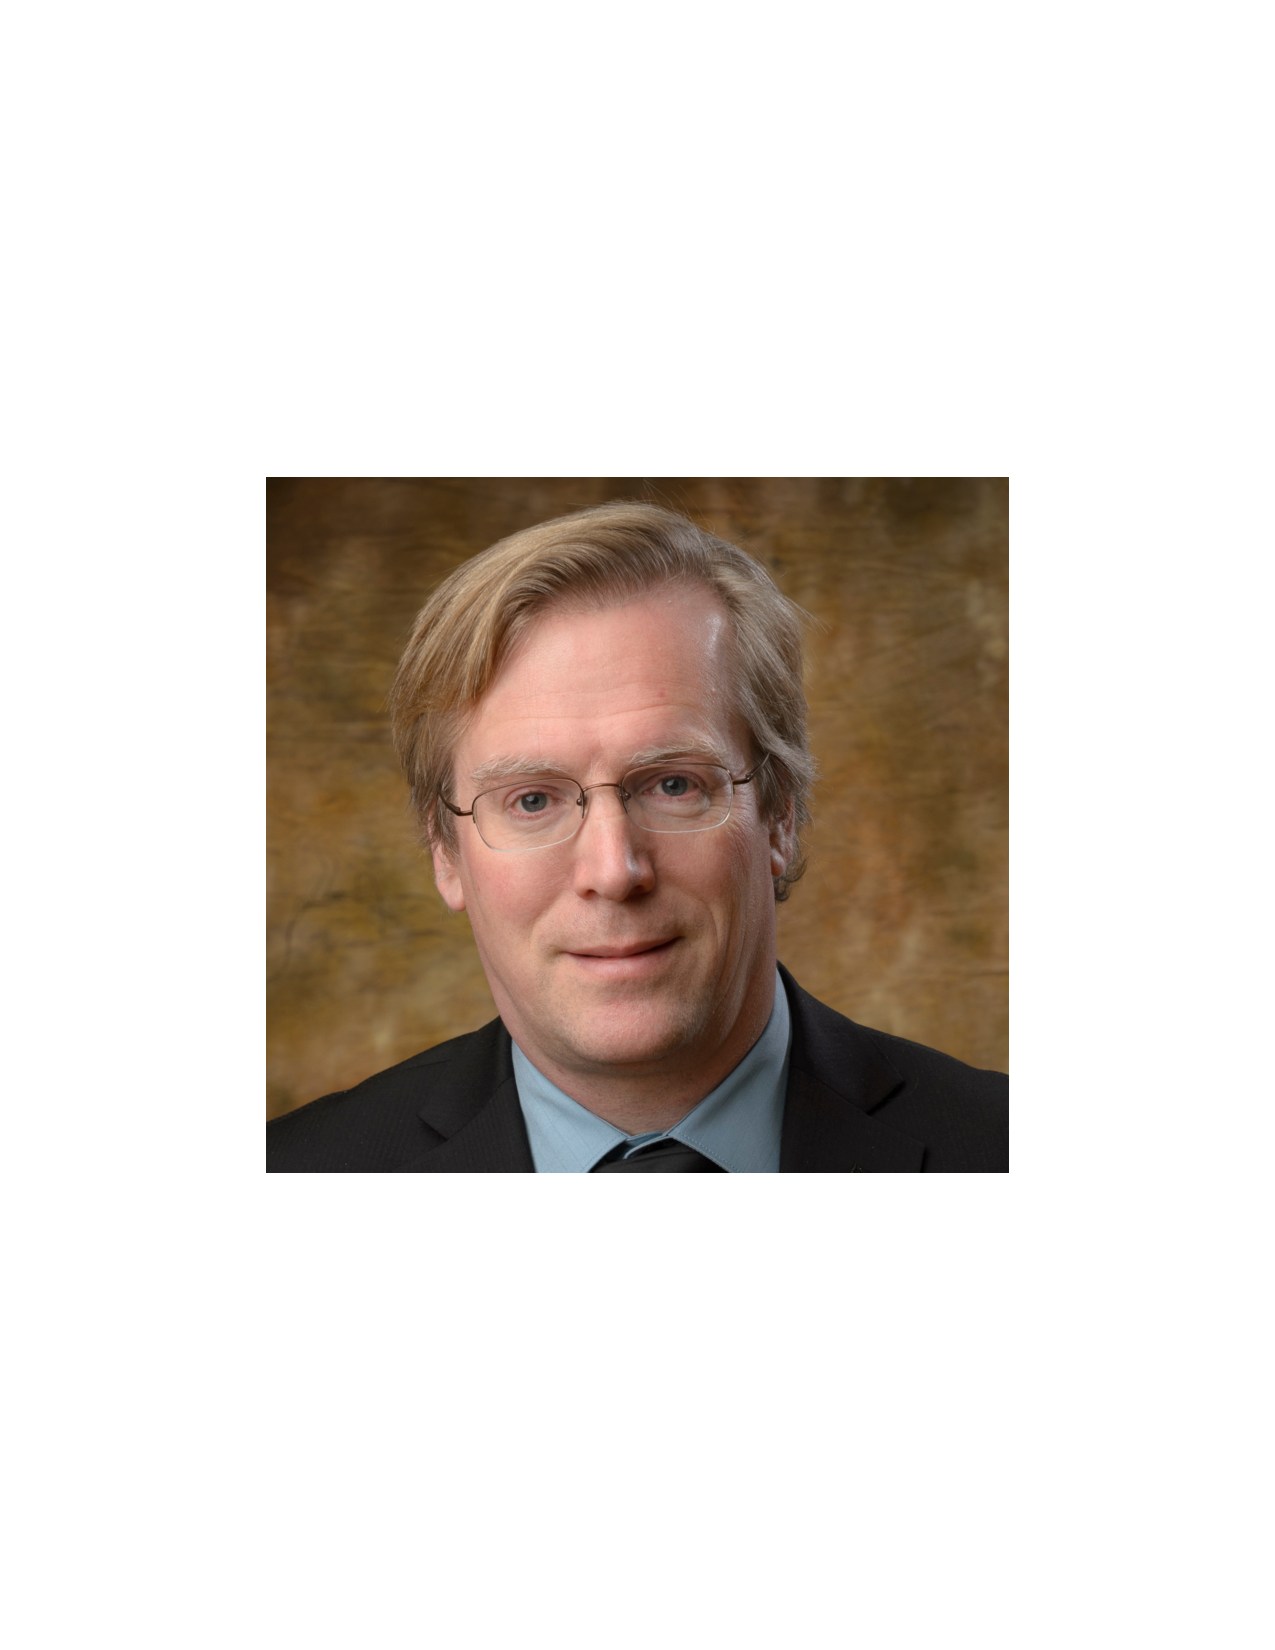
\includegraphics[width=1in,height=1.25in,clip,keepaspectratio]{pdf/AU908c.pdf}}]{James L. Garrison}
James L Garrison is an Associate Professor in the School of Aeronautics and Astronautics at Purdue University with a courtesy appointment in the School of Electrical and Computer Engineering. Previously he was employed by the NASA Goddard Space Flight Center in Greenbelt MD. He has a PhD in Aerospace Engineering Sciences from the University of Colorado Boulder and is the author or co-author of 33 peer-reviewed journal articles and 7 US Patents. He served as the Chair of GNSS+R 2012, an IEEE-NASA co-sponsored conference. 
Prof. Garrison's current research interests include Earth remote sensing using Global Navigation Satellite Systems (GNSS) and signals of opportunity. 
\end{IEEEbiography}

% You can push biographies down or up by placing
% a \vfill before or after them. The appropriate
% use of \vfill depends on what kind of text is
% on the last page and whether or not the columns
% are being equalized.

%\vfill

% Can be used to pull up biographies so that the bottom of the last one
% is flush with the other column.
%\enlargethispage{-5in}



% that's all folks
\end{document}